%%%% Main Thesis Style %%%%%%%%%%%%%%%%%%%%%%%%%%%%%%%%%%%%%%%%%%%%%%%%%%%%%%%%
\documentclass[12pt]{report}

%\usepackage[color=blue,width=3pt,height=0.5\baselineskip]{overcolored}

\usepackage{styles/suthesis-modified}


%%%% Packages %%%%%%%%%%%%%%%%%%%%%%%%%%%%%%%%%%%%%%%%%%%%%%%%%%%%%%%%%%%%%%%%%

% microtype for improved spacing and readability
\usepackage{microtype}

% lualatex-math to fix math typesetting packages with lualatex
\usepackage{lualatex-math}

% language stuff
%\usepackage{polyglossia}
%\setdefaultlanguage[variant=american]{english}
\usepackage[english=american]{csquotes} % english=american needed because polyglossia support is not good yet
\MakeOuterQuote{"}
\MakeAutoQuote{<}{>}

% cleveref needs to be before amsmath so equation references work
\usepackage{cleveref} % for smart reference ranges

% AMS math before other font stuff
\usepackage{amsmath}
\setcounter{MaxMatrixCols}{20} % default of 10 is too small
\usepackage{amsfonts} % Type1 CM, blackboard bold, Fraktur, and select symbols
\usepackage{amsthm} % add proof environment

% font stuff
\usepackage{fontspec} % enable access to system fonts
% Mapping=tex-text not supported yet in LuaTeX
%\defaultfontfeatures{Mapping=tex-text} % map TeX conventions for quotation marks, dashes to proper characters
%\defaultfontfeatures{Ligatures=TeX} % map TeX conventions for quotation marks, dashes to proper characters
% Renderer=Basic needed to fix bug with Times New Roman that prevents using dashes
\defaultfontfeatures{Renderer=Basic,Ligatures=TeX} % map TeX conventions for quotation marks, dashes to proper characters

%\setmainfont{STIXGeneral}
\setmainfont{Times New Roman}
%\setmainfont{Linux Libertine O} % open source Times New Roman look-alike
%\setmainfont{TeX Gyre Bonum} % expanded URW Bookman L, like Bookman
%\setmainfont{TeX Gyre Pagella} % expanded URW Palladio, like Palatino
%\setmainfont{TeX Gyre Schola} % expanded URW Century Schoolbook L, like Century Schoolbook
%\setmainfont{TeX Gyre Termes} % expanded URW Nimbus Roman No9 L, like Times New Roman

\setsansfont{TeX Gyre Heros} % expanded URW Nimbus Sans, like Helvetica
%\setsansfont{TeX Gyre Adventor} % expanded URW Gothic, like AvantGarde
%\setsansfont[Scale=MatchLowercase]{Linux Biolinum} % similar to Optima/URW Classico which pairs well with Palatino
% \setsansfont[Scale=MatchLowercase]{Linux Biolinum O} % similar to Optima/URW Classico which pairs well with Palatino

%\setmonofont{}

%\usepackage{unicode-math} % needed to specify math font
%\setmathfont{Latin Modern Math} % OpenType version of Computer Modern
%\setmathfont{XITS Math} % use with Times
%\setmathfont{Asana Math} % use with Palatino/URW Palladio/TeXGyrePagella
%\setmathfont{TeX Gyre Bonum Math} % use with URW Bookman L/Bookman
%\setmathfont{TeX Gyre Pagella Math} % use with URW Palladio/Palatino
%\setmathfont{TeX Gyre Schola Math} % use with URW Century Schoolbook L
%\setmathfont{TeX Gyre Termes Math} % use with URW Nimbus Roman No9 L/Times New Roman

% bibliography
\usepackage{styles/mybiblatex-chicago}
\addbibresource{references.bib}

% graphics
\usepackage{graphicx}
\DeclareGraphicsExtensions{.pdf,.png,.jpg}
\usepackage{tikz}
\tikzstyle{image}=[inner sep=0pt]

% other packages
\usepackage{mathtools} % for math stuff not provided by AMSmath
\usepackage[margin=10pt,labelfont=bf,labelsep=endash]{caption}
\usepackage{subcaption} % for subfigures
\usepackage[neverdecrease]{paralist} % for in-paragraph lists and tightly-spaced lists
\usepackage{array} % advanced table features like specifying column width
\usepackage{booktabs} % for cleaner tables
\usepackage{tabu} % for tables with fixed total width
\usepackage{algorithmic} % for algorithmic environment
\algsetup{indent=2em}
\newcommand{\GIVEN}{\STATE \textbf{given} }
\usepackage[ruled]{algorithm} % for algorithm float
\usepackage{nowidow} % for preventing widow and orphan lines, does nothing by default
\setnowidow % do not allow single lines at beginning of page

% hyperlinks, load after everything else (especially biblatex)
\usepackage{hyperref}
\hypersetup{colorlinks,urlcolor=black,citecolor=black,filecolor=black,linkcolor=black}
\urlstyle{rm} % remove typewriting styling from links


%%%% Macros %%%%%%%%%%%%%%%%%%%%%%%%%%%%%%%%%%%%%%%%%%%%%%%%%%%%%%%%%%%%%%%%%%%

\newcommand{\pkg}[1]{\texttt{#1}}

\makeatletter
\def\blfootnote{\xdef\@thefnmark{}\@footnotetext}
\makeatother

\newenvironment{italicquote}{%
  \quote
  \itshape
}{%
  \endquote
}

\DeclareMathOperator*{\argmin}{arg\,min}
\DeclareMathOperator{\grad}{\mathbf{grad}}
\DeclareMathOperator{\prox}{\mathbf{prox}}
\DeclareMathOperator{\soft}{\mathbf{soft}}
\DeclareMathOperator{\bsoft}{\mathbf{bsoft}}
\DeclareMathOperator{\shrink}{\mathbf{shrink}}
\DeclarePairedDelimiter{\paren}{(}{)}
\DeclarePairedDelimiter{\brak}{[}{]}
\DeclarePairedDelimiter{\set}{\{}{\}}
\DeclarePairedDelimiter{\abs}{\lvert}{\rvert}
\DeclarePairedDelimiter{\nrm}{\lVert}{\rVert}
\DeclarePairedDelimiter{\floor}{\lfloor}{\rfloor}
\DeclarePairedDelimiter{\ceil}{\lceil}{\rceil}
%\DeclarePairedDelimiterXPP{\norm}[2]{}{\lVert}{\rVert}{_{#1}}{#2} % requires new mathtools
\DeclarePairedDelimiterX{\innerprod}[2]{\langle}{\rangle}{#1,#2}

% for cyrillic Sha:
% solution 1, fake it
%\newcommand{\Sha}{\mathrm{III}}
% solution 2, using unicode-math commands (must use lualatex or xelatex)
% and requires math font with character in it (Latin Modern doesn't)
%\ExplSyntaxOn
%\newcommand{\mathcyrillic}[2]{%
%\chardef#1=#2
%\um_set_mathcode:nnnn{#1}{\mathalpha}{\um_symfont_tl}{#2}}
%\ExplSyntaxOff
%\mathcyrillic{\Sha}{"0428}
% solution 3, load the font and character manually
\DeclareFontFamily{U}{wncy}{}
\DeclareFontShape{U}{wncy}{m}{n}{<->wncyr10}{}
\DeclareSymbolFont{cyrletters}{U}{wncy}{m}{n}
\DeclareMathSymbol{\Sha}{\mathalpha}{cyrletters}{"58}

\usepackage{styles/mathcommands-private}


%%%% Thesis Info %%%%%%%%%%%%%%%%%%%%%%%%%%%%%%%%%%%%%%%%%%%%%%%%%%%%%%%%%%%%%%

\title{Theory and application of sparsity for radar sensing of ionospheric plasma}
\author{Ryan Volz}
\dept{Aeronautics and Astronautics}
\principaladvisor{Sigrid Close}
\firstreader{Philip J. Erickson}
\secondreader{Mykel Kochenderfer}
\viceprovost{Patricia J. Gumport}
\submitdate{December 2014}
\licensedeclaration{%
 \begin{tabu} to \textwidth {X[-1,l,m]X[J,m]}
  
\includegraphics{license_cc_by-nc} & This work is licensed under a Creative Commons Attribution-NonCommercial 4.0 International License. \newline\url{http://creativecommons.org/licenses/by-nc/4.0/}
 \end{tabu}
}
\onlineat{\url{http://purl.stanford.edu/kw265jg4383}}
\onlinecopyrighttrue
\completedsignaturetrue

\makeatletter
\hypersetup{pdftitle=\@title}
\hypersetup{pdfauthor=\@author}
\makeatother
\hypersetup{pdfkeywords=radar; sparsity; inversion; compressed sensing; ionosphere; meteor; pulse compression; pulse coding; waveform coding}

%%%% Body %%%%%%%%%%%%%%%%%%%%%%%%%%%%%%%%%%%%%%%%%%%%%%%%%%%%%%%%%%%%%%%%%%%%%

\begin{document}

% preface
\beforepreface
\prefacesection{Abstract}
The ionosphere plays an important role in the geospace system, perturbing and disrupting radio signals that pass through it and coupling the Earth with its space environment. Of particular note to spacecraft designers and operators are the small meteoroids that routinely impact spacecraft and are observable due to their passage through the ionosphere. Mechanical and electrical damage due to hypervelocity impacts with meteoroids pose a significant threat to spacecraft, and to fully characterize the threat it is necessary to observe the sporadic meteoroids through the meteor plasma that they create in the ionosphere. These observations, in addition to those of ionospheric plasmas that disrupt communications, can be made with high-power large-aperture radars located across the globe. Unfortunately, current radar techniques are not sufficient for elucidating the details of these plasmas due to inherent signal processing artifacts.

Sparsity has recently gained prominence in many scientific fields as a means of speeding, simplifying, or increasing the accuracy of information processing. Often this research falls under the moniker of \emph{compressed sensing}, which exploits sparsity, global measurement, and nonlinear reconstruction to acquire data faster or with higher resolution. Mathematically, signals like images, sound waves, or radar returns can be represented with vectors. The vectors are paired with a dictionary describing atoms that, when combined according to the vector elements, can represent any given signal. Working with vectors gives a concrete definition of sparsity; it means that most of a vector's elements are zero. Natural phenomena tend to have structure, and that structure manifests itself as sparsity in the signal's vector representation with an appropriate dictionary. Knowing that natural signals are sparse allows one to constrain solutions to underdetermined measurements and uniquely find the signal's true representation.

In order to enable flexible high-resolution measurements of ionospheric plasma phenomena, a sparsity-based radar waveform inversion technique is formulated and found to eliminate processing artifacts caused by the standard matched filter approach. Taking direction from the theory of compressed sensing, sparsity of the radar target scene is employed as prior knowledge to successfully perform the inversion. The result is cleaner data that limits self-interference of range-spread targets and enables differentiation in crowded and variable environments. Though the approach has been applied to ionospheric radar, it is generally applicable and especially relevant for radar target scenes with multiple or distributed scatterers.

As a basis for the technique, a discrete radar model that captures signal sparsity in a delay-frequency dictionary is developed. This model is shown to have a strong connection to existing methods, resulting in an intuitive interpretation of the inversion technique as an iterative thresholding matched filter. An explicit formulation of the discrete model's representation of arbitrary distributed scatterers is derived, and it shows that sparsity is reasonably preserved in the discrete representation. Building on top of the model, waveform inversion is implemented using modern convex optimization techniques tailored for efficient computation and quick convergence. Finally, the real-world flexibility and effectiveness of the inversion technique is demonstrated by the elimination of filtering artifacts from meteor observations made with a variety of standard radar waveforms.

\newpage

\prefacesection{Acknowledgments}
In terms of both scholarly and personal support, this dissertation would not have been possible without the help of many people. I would like to thank my thesis committee members, Professors Mykel Kochenderfer, Stephen Boyd, and Charbel Farhat, for providing many interesting discussions and taking the time to critique this work. I would also like to thank the researchers and staff of the Jicamarca Radio Observatory, particularly Dr. Jorge Chau and Karim Kuyeng, for hosting me and running my experiments. At Stanford, the Space Environment and Satellite Systems lab has been my home for most of my graduate studies, and I would like to thank its past and present members for making that home a good one. Thanks must also go to my classmates and friends in the Aero/Astro department, particularly my study group, Tom Coles, Brandon Fetroe, and Jason Forshaw, and my quals group, Brandon Morgan and Surajit Roy.

My first crash course in radar came on a two-week visit to the MIT Haystack Observatory to collect data and attend the AMISR workshop. I knew almost nothing about collecting and processing radar data at that point in time, but after those two weeks I knew enough to be dangerous. Credit and thanks go to the teachers at the workshop and the researchers at Haystack, most notably my co-advisor of sorts, Dr. Phil Erickson. On the first day of that visit, Phil sat me down in his office, gave my some Python code (with me never having used the language before), and let me go at it. He has answered my questions ever since, providing insight whenever I've been stuck on the thorny details of radar. I would like to thank Phil for being an outstanding teacher and mentor.

I was fortunate enough to be at the right place at the right time when I met my advisor, Professor Sigrid Close. Again, I knew nothing about radar or the ionosphere before that first meeting almost five years ago, and I had been beginning to wonder whether I would be able to find a good fit for my interests at Stanford. Sigrid solved those problems by providing me with ALTAIR meteor data to analyze and giving me the freedom to explore. She was enthusiastic and supportive when I later came to her office with ambitious ideas about applying compressed sensing to radar, even if it meant that I never actually got around to analyzing that ALTAIR data. I would like to thank Sigrid for providing many work and travel opportunities and for guiding my scholarly explorations with the perfect blend of support and advice.

Finally, I would like to thank my friends and family for their encouragement, especially for not asking too many questions about when this thesis would finally be done. Most importantly, though, I want to thank my wife, Bekah, without whom none of this would have happened. It has been a long journey to get to this point, and I'm glad I could share the highs and lows with her.

\begin{flushright}
 \textit{Ryan Volz}\\
 \textit{Stanford, California}\\
 \textit{December, 2014}
\end{flushright}

\vfill
\noindent
\begin{minipage}{\textwidth}
 \footnotesize%
 This research was supported by the Department of Defense (DoD) through the National Defense Science \& Engineering Graduate Fellowship (NDSEG) Program, and by the National Science Foundation under Grant No. AGS-1056042.
\end{minipage}
\afterpreface

% chapters
\part{Introduction}
\label{part_introduction}
\graphicspath{{chapters/introduction/figures/}}
\chapter{Introduction}
\label{introduction}
The fundamental mechanism of radar is to transmit a radio signal and listen for reflections to gain information about remote targets. Although the concept of radar was evident from the beginnings of electromagnetic theory, it was not until sufficient transmitter and receiver technology was developed around the time of World War II that practical radars came into use for remote detection of ships and aircraft \autocite{Sko01}. Following the war, radar use branched out from military applications into scientific and commercial fields. Radar is still used with remote targets like aircraft and satellites for detection, tracking, and imaging, but it is more commonly encountered as a tool in weather or in highway speed limit enforcement \autocite{MS14}. Less known are the applications that drive the development of radar today, including autonomous landing systems for aircraft, driver-less cars, and terrain mapping (both surface and underground) of the Earth and other planets \autocite{Jol09, MS12}. But of the many uses of radar, one is somewhat unique in its requirements: the study of ionospheric plasmas. These plasmas vary widely in size, density, and persistence, so their study has necessitated the development of transmission coding and signal processing techniques that are adaptable to a wide range of circumstances. Unfortunately, the current techniques produce inherent processing artifacts or are inflexible in their application, limiting our ability to learn more about some ionospheric plasmas \autocite{VLV08a}.

The goal of this thesis is to develop new methods for radar data analysis that enable flexible, high-resolution measurements of ionospheric plasma phenomena. The key to achieving this goal lies in leveraging the concept of sparsity; scenes typically observed by a radar have a simple representation relative to the space of possible signals, and this prior information can help to improve measurements and analysis. In the case of measurements, this thesis presents a waveform inversion technique for removing ambiguity and self-interference due to the transmitted signal. In the case of analysis, a clustering method is developed for automatically detecting and classifying related scattering events. For events with a single point scatterer, we simulate and analyze statistics of matched filter interpolation for estimating target range and range-rate with increased resolution. Though the ionosphere provides the motivation and application for this work, the research is primarily focused on techniques that are generally applicable to most radar scenarios, especially those with multiple or distributed scatterers.

The remainder of this chapter broadly covers the ionosphere, radar, and sparsity in order to motivate the research and set the stage for later developments. Section \ref{intro_ionosphere} gives background information on the ionosphere and describes its effects on radio communications, its role in studying the science of the geospace system, and its function in observing meteoroids that pose a threat to orbiting satellites. Section \ref{intro_radar} describes the radars used to study the ionosphere, the types of scattering that are typically encountered, and the challenges they present. Section \ref{intro_sparsity} details the function of sparsity in efficient information processing and its emerging role in many different fields of research. Finally, Section \ref{contributions} outlines the contributions of this dissertation, and Section \ref{outline} provides a reader's guide for the remaining chapters.

\section{The Ionosphere}
\label{intro_ionosphere}
Surrounding the Earth is a region defined by ionization: the ionosphere. It is a portion of the upper atmosphere where charged particles, both electrons and ions, are present in addition to neutral air molecules. This region extends from approximately 60 km to 2000 km in altitude, a range which includes the low Earth orbits (LEO) inhabited by the majority of satellites. The ionized and neutral particles constitute a plasma, one that varies greatly over time and over the spatial extent of the ionosphere. Driving these variabilities are interactions with the lower atmosphere and the space environment, most notably radiation from the sun. As the interface between space and the Earth's atmosphere, the ionosphere is difficult to study but critically important for understanding the geospace system \autocite{CEDAR11}.

\subsection{Formation and Variability}
\label{intro_ionosphere_formation}
Ionization of neutral air molecules by solar radiation is the primary cause for the existence of the ionosphere, and it is balanced by ion-electron recombination chemistry. Recombination limits the maximum ionized plasma density during the day and dissipates the plasma at night. Naturally, the temporal peak in plasma density happens near noon when the ionization rate is at its highest, but even then the plasma density is at most around one percent of the neutral background. Example plasma densities for the daytime and nighttime mid-latitude ionosphere are shown in Figure \ref{fig:ionospheric_density}.
\begin{figure}[tpb]
 \centering
 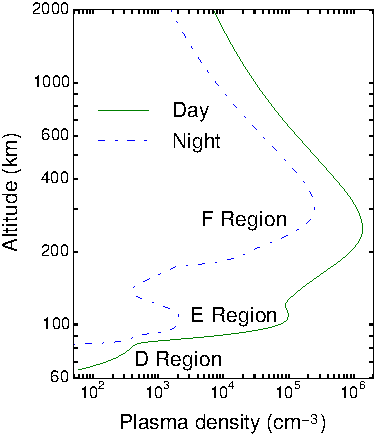
\includegraphics{ionospheric_density}
 \caption[Ionospheric plasma density during day and night]{\emph{Ionospheric plasma density during day and night.} This plot shows predicted electron density at noon and midnight on December 1, 2014, according to the IRI-2012 model \autocite{BAZ+14}. The prediction is for the mid-latitude ionosphere above the Millstone Hill incoherent scatter radar.}
 \label{fig:ionospheric_density}
\end{figure}%
Solar radiation ionizes air molecules down to altitudes of approximately 60 km, forming the ionosphere's lower boundary. Its upper boundary at approximately 2000 km altitude is more tenuously defined; it is not a cutoff of ionization but rather one of sufficient density to exhibit bulk plasma properties. Between these boundaries, the ionosphere is divided by altitude into different regions defined by variations in plasma density. Arranged by increasing altitude, these layers are called the D, E, and F regions. The different regions exist because the ionization rate varies with altitude: solar intensity decreases with decreasing altitude as more radiation is absorbed, while at the same time the neutral atmosphere increases in density and varies in composition with decreasing altitude due to gravity \autocite{Tas10, Kel09}.

Though this simple model is useful to conceptualize the ionosphere, it is important to note that the ionosphere is part of a complex geospace system and therefore exhibits significant variability over time and space. Day/night variability has already been mentioned, but tidal, seasonal, and solar activity cycles are also significant drivers of the ionosphere. Weather is an important contributor on shorter timescales, both in terms of atmospheric weather from the dynamics of the neutral atmosphere and space weather from the flares and particle precipitation of solar storms. In terms of spatial variability, the changing orientation of the Earth's magnetic field lines with respect to latitude divides ionospheric behavior into three regions: equatorial, polar, and mid-latitude. In the equatorial region, the magnetic field lines are horizontal. This results in unique plasma dynamics that include the equatorial electrojet current sheet, turbulence-induced field-aligned irregularities, and equatorial bubbles \autocite{Kel09}. In the polar region, the magnetic field lines connect to the magnetosphere and solar wind and bring a supplemental source of energetic particles. The result is enhanced ionization and light displays known as aurora, among other phenomena \autocite{KR95}. The mid-latitude region lies between the other two and is defined through the absence of equatorial and polar effects. Boundary interactions are characteristic of this region, including the plasmasphere boundary layer of the sub-auroral zone \autocite{CL04} and notable disturbances like sudden stratospheric warming \autocite{GHB+13}.

\subsection{Communications and Irregularities}
\label{intro_communications}
The ionosphere is felt most strongly in daily life through its effects on radio communications. Radio waves of lower frequency (less than about 13 MHz for a typical F-region peak plasma density \autocite{Tas10}) reflect off of the ionosphere. In practical terms, AM radio broadcasts reflect (when they are not absorbed), while the higher-frequency FM radio signals pass through the ionosphere into space. However, even the higher microwave-frequency signals that are typically used for satellite communications are subject to attenuation, refraction, and delay \autocite{Kel09}. This is especially important to consider in the case of the global navigation satellite systems (GPS, GLONASS, Galileo); these depend on precise timing and require correction for ionospheric effects in order to achieve high positioning accuracy.

Ionospheric irregularities are even more important to characterize, due to their unpredictability and potential to completely disrupt typical satellite communications. Random variation of signal strength and phase, termed scintillation, occurs whenever there are abrupt changes in electron density along the signal path. These irregularities cause scattering and self-interference of a radio signal, a process analogous to looking through rough glass. The result is corrupted communication or even loss of signal. Figure \ref{fig:scintillation} depicts the measured signal for a radar beam sweeping back and forth across a calibration target.
\begin{figure}[tpb]
 \centering
 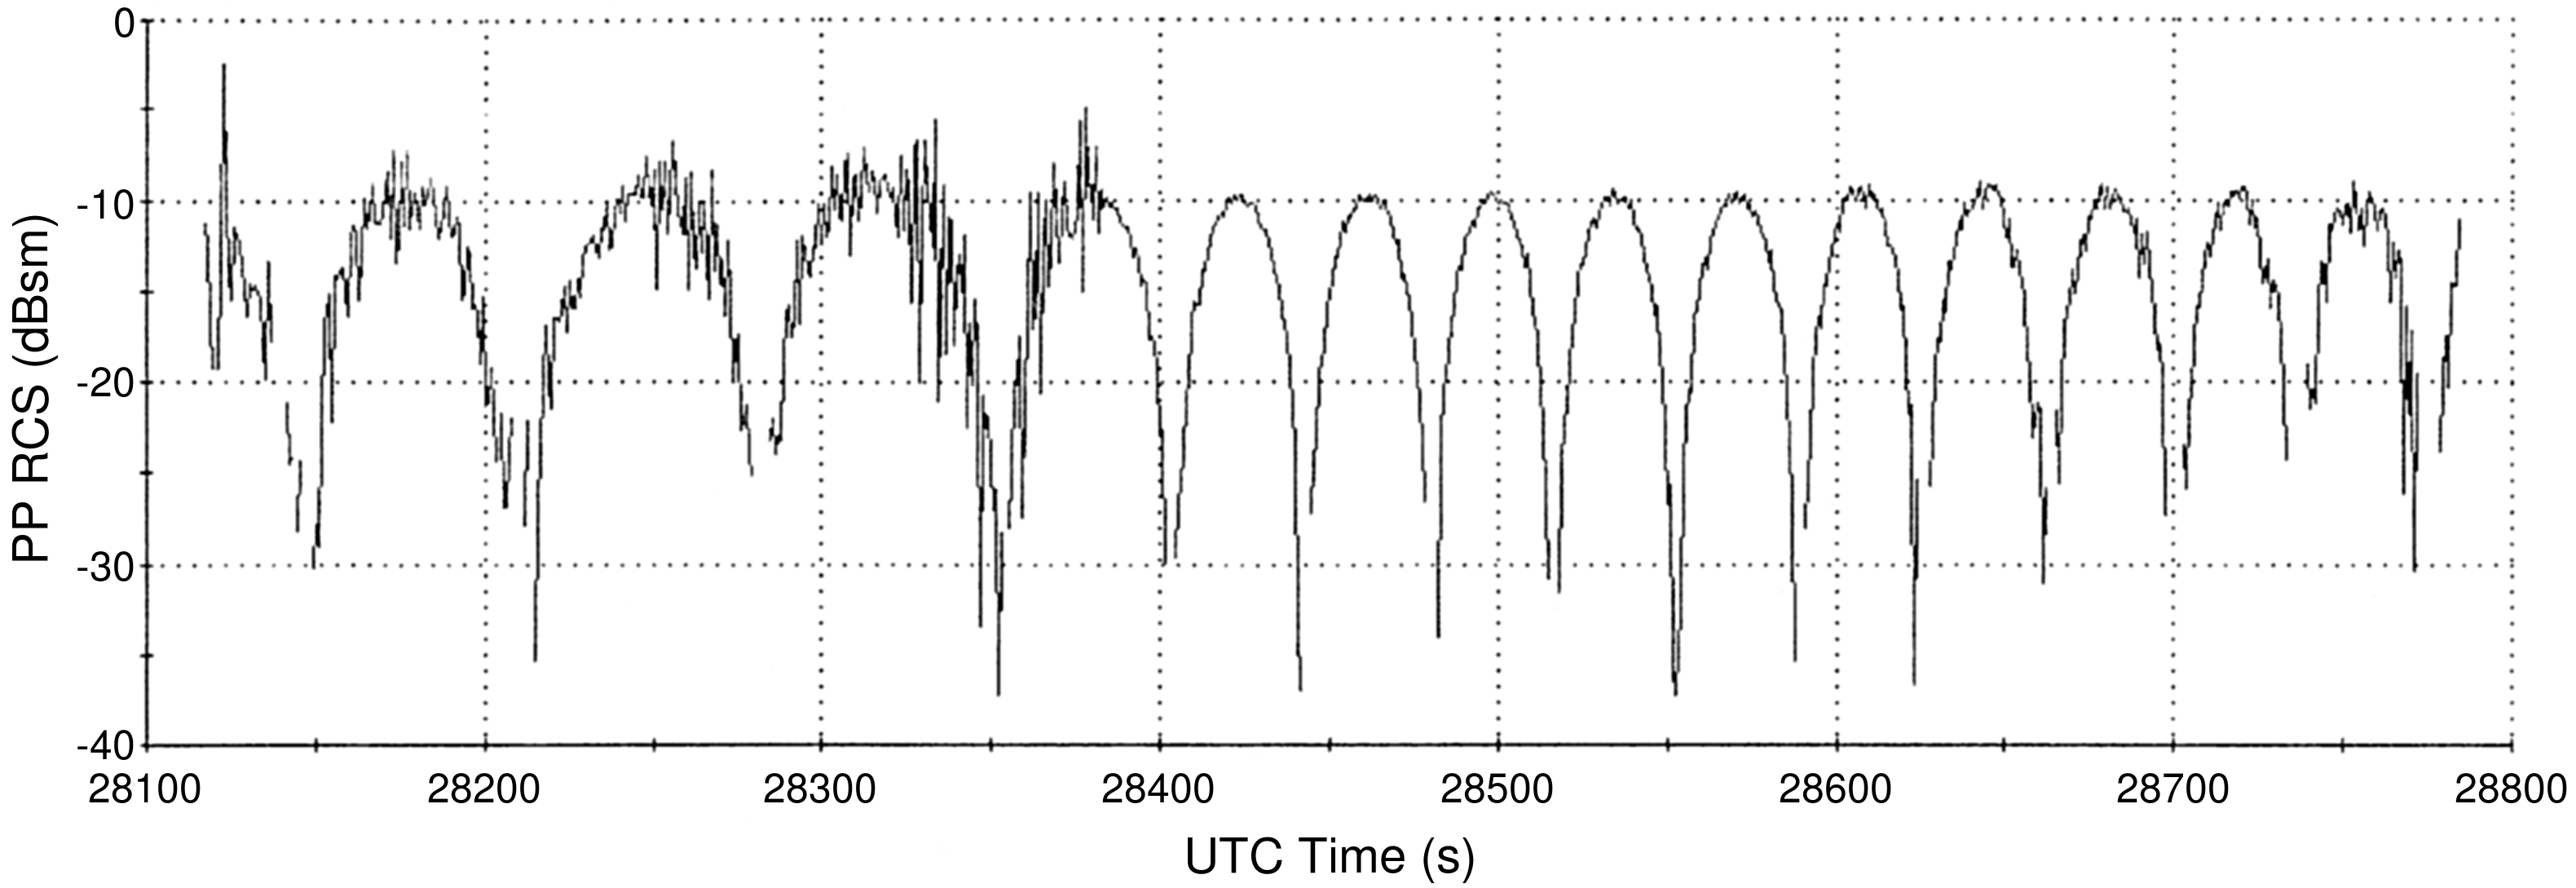
\includegraphics{scintillation}
 \caption[Scintillation of a radar calibration signal]{\emph{Scintillation of a radar calibration signal.} This plot shows the radar cross section (RCS) measured for the principal polarization (PP) from a calibration test with the ALTAIR radar at 160 MHz. The radar beam was swept back and forth across a fixed target, so the signal strength is expected to be consistent with each pass. Scintillation is evident on the first four and a half passes, while the rest are nearly scintillation-free.}
 \label{fig:scintillation}
\end{figure}%
The first four passes exhibit scintillation as strong variations in signal strength, while the remaining passes are nearly scintillation-free. Though categorized as an irregularity, scintillation is an everyday occurrence arising from typical variation of the ionosphere. Geomagnetic storms, in contrast, are truly irregular occurrences arising from solar activity. They disrupt the ionosphere by increasing direct energy input and transport effects, thus triggering further irregularities and scintillation \autocite{Kel09}.

\subsection{System Science}
\label{intro_system_science}
Given how much the world depends on satellite communications and radio systems, studying the ionosphere in order to predict and mitigate disruptions is clearly important. In order to do that, though, it is necessary to examine the ionosphere's role in the overall geospace system. This system is formed of complex interactions between the Earth, with its atmosphere and magnetic field, and the space environment, with the dominating influence of the Sun. Scientific study of the geospace system in the past has been limited by the inability to investigate its complexity, eloquently described by the \textcite{CEDAR11} as the "many interacting elements that, as a whole, exhibit properties not obvious from the properties of the individual parts." Nevertheless, this so-called systems science is becoming more feasible every day with the advancement of computational and measurement techniques. Since the ionosphere is a key cog in the geospace system, it is important to develop new methods for studying the ionosphere that embrace complexity and enable improved understanding of the system as a whole. This requires measurements that are universal, encompassing large portions of the ionosphere, and it requires techniques that are flexible, measuring plasmas spanning a wide range of size, density, and persistence.

\subsection{Meteoroids and Meteors}
\label{intro_meteoroids}
Of the many components of the space environment that interact with the ionosphere, meteoroids warrant special mention. \emph{Meteoroid} is a term that encapsulates any small, naturally occurring solid body in space. Meteoroids range in size from 10 micrometers to approximately 1 meter in diameter; smaller particles are called dust, and larger bodies are called asteroids \autocite{RG10}. While an asteroid crossing paths with the Earth is a rare event of global disaster proportions, meteoroids routinely enter the Earth's atmosphere. Furthermore, meteoroids are more common as size decreases; roughly speaking, their number are inversely proportional to the mass of the meteoroid squared as shown in Figure \ref{fig:meteoroid_mass_distribution}.
\begin{figure}[tpb]
 \centering
 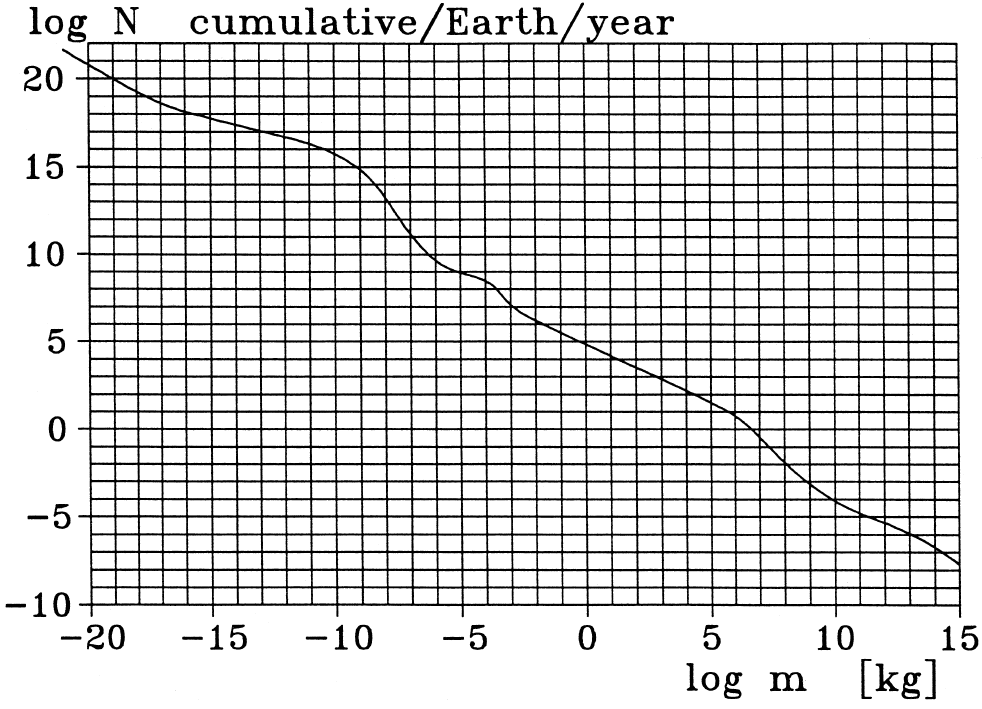
\includegraphics[width=0.6\textwidth]{ceplecha_meteoroid_count_vs_mass}
 \caption[Cumulative distribution of interplanetary bodies as a function of mass]{\emph{Cumulative distribution of interplanetary bodies as a function of mass.} This plot, reproduced from \textcite{CBE+98}, shows the cumulative count $N$ of interplanetary bodies (including meteoroids and asteroids) with mass greater or equal to $m$ that enter the Earth's atmosphere per year. Both the count and mass are plotted as base-10 logarithms.}
 \label{fig:meteoroid_mass_distribution}
\end{figure}%
As a point of reference, on the order of 100 million meteoroids big enough to be detected by high-power large aperture radars (0.1 micrograms or larger \autocite{CBC+07}) are estimated enter the Earth's atmosphere every second on average \autocite{CBE+98}; this is equivalent to approximately one meteoroid every second within a radar beam that is pointed upward with a one degree half-power beamwidth. If a meteoroid survives passage through the atmosphere and lands on the Earth, which is correspondingly more rare, the surviving body is called a \emph{meteorite}.

The term \emph{meteor} is not to be confused with meteoroid, although they are often incorrectly used interchangeably. A meteor denotes the plasma created by a meteoroid as it speeds through the atmosphere, typically forming between 80 and 120 km in altitude. Sometimes light is emitted when the meteoroid is large or fast enough, and this is also called a meteor or colloquially a shooting star. Meteoroids enter the atmosphere with such speed, typically between 11 and 72 km/s \autocite{CBE+98}, that they heat up, ablate their constituents, and cause some of the surrounding air to ionize. The resulting plasma is many times denser than the background ionospheric plasma, but it typically only retains that density for a fraction of a second before diffusing and recombining \autocite{Jon95, DWB+08}. The plasma dynamics spurred by meteors are significant to the overall ionospheric system, while the ablated meteoroid elements play an important role in the chemistry of the upper atmosphere.

Aside from their role in driving ionospheric processes, meteoroids are also important because of the likelihood that they will impact satellites. The most prevalent meteoroids are small enough ($<$ 1 microgram) that they can't do physical damage; however, meteoroids travel fast enough that even the smaller ones can cause electrical damage to satellites through the plasma that they create upon impact \autocite{CCC+10}. \textcite{LCG+13} showed through ground experiments that this damage is possible and could explain nebulously-attributed or otherwise unexplained anomalies and failures of a number of satellites. In order to better characterize the electrical threat to satellites, we need better methods of remotely measuring the meteoroid distributions of rate, size, speed, and composition; the best way to do that is by advancing radar techniques for observing meteors.

\section{Radar Measurements}
\label{intro_radar}
Due to its remoteness and size, spanning altitudes from 60 km to 2000 km, the ionosphere is difficult to study. Even the lowest reaches of the ionosphere are outside the range of aircraft, leaving balloons, rockets, and satellites as the only carriers for \emph{in situ} measurement equipment. Not only are these methods expensive, but they also do not give enough data over time and space to perform more than localized studies. For large-scale observation of the ionosphere, scientists are left with methods of remote sensing, particularly radar.

\subsection{Incoherent Scatter Radars}
\label{intro_isrs}
It takes a large radar to be sensitive enough to measure scattering from electrons in the background ionosphere; this type of signal is called incoherent scatter, and these large radars are incoherent scatter radars (ISRs) \autocite{Gor58}. There are only about a dozen ISRs in operation across the globe, with locations depicted in Figure \ref{fig:isr_map}.
\begin{figure}[ptb]
 \centering
 \begin{subfigure}{\textwidth}
  \centering
  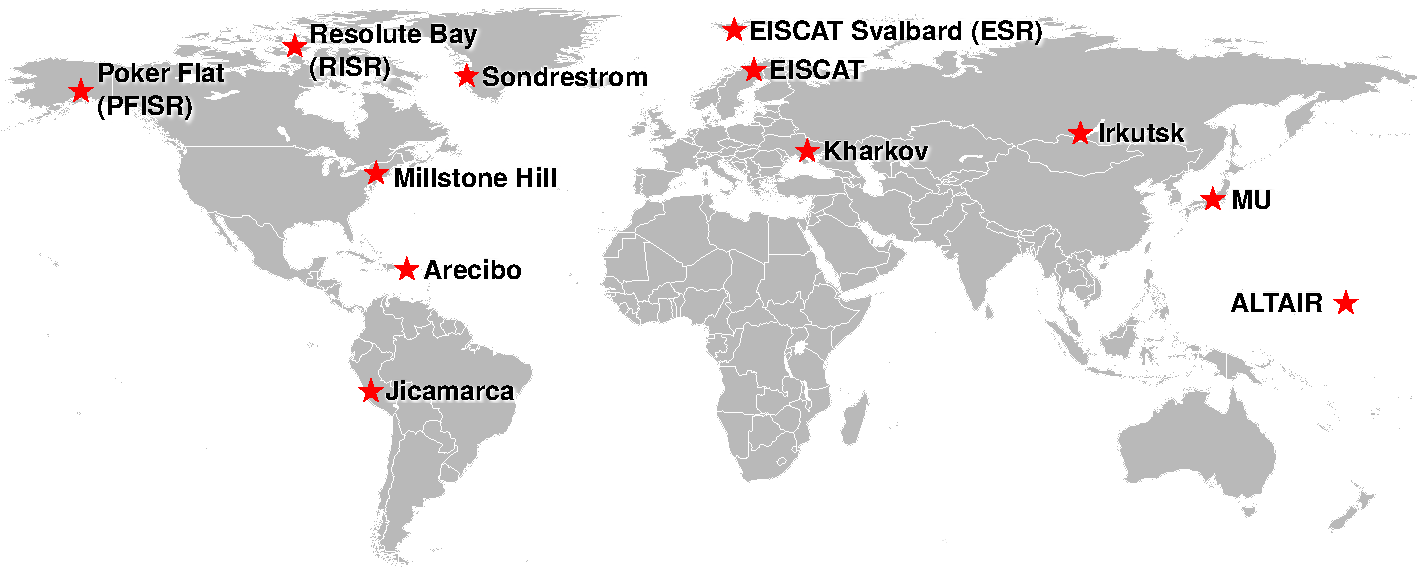
\includegraphics[width=0.9\textwidth]{isr_map}
  \caption{Map of Incoherent Scatter Radars (ISRs)}
  \label{fig:isr_map}
 \end{subfigure}
 \begin{minipage}[b]{0.49\textwidth}
 \begin{subfigure}[b]{\textwidth}
  \centering
  \includegraphics[width=\textwidth,trim=0px 20px 0px 105px,clip]{jicamarca}
  \caption{Jicamarca ISR}
  \label{fig:jicamarca}
 \end{subfigure}
 \begin{subfigure}[b]{\textwidth}
  \centering
  \includegraphics[width=\textwidth]{pfisr}
  \caption{Poker Flat ISR (PFISR)}
  \label{fig:pfisr}
 \end{subfigure}
 \end{minipage}
 \begin{subfigure}[b]{0.49\textwidth}
  \centering
  \includegraphics[width=\textwidth]{millstone_hill_radar}
  \caption{Millstone Hill ISR}
  \label{fig:millstone}
 \end{subfigure}
 \caption[Incoherent scatter radars spanning the globe]{\emph{Incoherent scatter radars spanning the globe.} Locations of the current ISRs are shown in \textbf{(\subref{fig:isr_map})}. The Jicamarca ISR \textbf{(\subref{fig:jicamarca})} is a phased array of dipole antennas located outside of Lima, Peru. The Poker Flat ISR \textbf{(\subref{fig:pfisr})} is a modern phased array located in Poker Flat, Alaska. The Millstone Hill ISR \textbf{(\subref{fig:millstone})} is composed of one steerable dish antenna and one fixed zenith dish antenna and is located outside of Boston, Massachusetts.}
 \label{fig:isrs}
\end{figure}%
Each radar covers a small slice of the ionosphere ranging from equatorial latitudes (e.g. Jicamarca outside Lima, Peru; Figure \ref{fig:jicamarca}) through mid-latitudes (e.g. Millstone Hill near Boston, MA; Figure \ref{fig:millstone}) to polar latitudes (e.g. the Poker Flat ISR in Alaska; Figure \ref{fig:pfisr}). The main parameters of the various ISRs are given in Table \ref{tab:isr_parameters}.
\begin{table}[tb]
 \renewcommand{\arraystretch}{1.2}
 \begin{center}
 \caption[Incoherent scatter radar parameters]{\emph{Incoherent scatter radar parameters.}}
 \label{tab:isr_parameters}
 \begin{tabular}{@{}llllll@{}} % @{} removes space from edge
  \toprule
  Radar & Frequency & Bandwidth & Peak Power & Gain & Size\\
  & (MHz) & (MHz) & (MW) & (dBi) & (m)\\
  \midrule
  ALTAIR\footnotemark[1] & 160/422 & 7/18 & 6 & 34/42 & 46\\
  Arecibo\footnotemark[2] & 430 & 1 & 2.5 & 62 & 305\\
  EISCAT VHF\footnotemark[3] & 224 & 1 & 1.6 & 46 & 120 $\times$ 40\\
  EISCAT UHF\footnotemark[3] & 931 & 1 & 2 & 48.1 & 32\\
  ESR\footnotemark[3] & 500 & 1 & 1 & 42.5/45 & 32/42\\
  Irkutsk\footnotemark[4] & 154 & 0.014 & 3.2 & 35 &\\
  Jicamarca\footnotemark[5] & 50 & 1 & 4.5 & 42.6 & 300 $\times$ 300\\
  Kharkov\footnotemark[6] & 158 & 0.015 & 2 & 40 & 100\\
  Millstone\footnotemark[7] & 440 & 1 & 2.5 & 42.5/45.5 & 46/68\\
  MU\footnotemark[8] & 46.5 & 1.65 & 1 & 34 & 103\\
  PFISR\footnotemark[9] & 450 & 1 & 2 & 43 & 30 $\times$ 30\\
  RISR\footnotemark[10] & 442.5 & 1 & 2 & 43 & 30 $\times$ 30\\
  Sondrestrom\footnotemark[11] & 1290 & 1 & 3 & 50 & 32\\
  \bottomrule
 \end{tabular}
 \end{center}
 
 \footnotesize
 [\footnotemark[1]\cite{TBOT79}; \footnotemark[1]\cite{CHMM02}; \footnotemark[2]\cite{Hag05}; \footnotemark[3]\cite{EISCAT_SPEC}; \footnotemark[4]\cite{PMZ+08}; \footnotemark[5]\cite{Och63}; \footnotemark[5]\cite{JICAMARCA_SPEC}; \footnotemark[6]\cite{BTC06}; \footnotemark[7]\cite{Eva65}; \footnotemark[7]\cite{MILLSTONE_SPEC}; \footnotemark[8]\cite{FST+85}; \footnotemark[9]\cite{CGHN09}; \footnotemark[9]$^{,}$\footnotemark[10]\cite{AMISR_SPEC}; \footnotemark[11]\cite{KHVV95}]
\end{table}%
Most of their characteristics are roughly similar, with megawatt-class transmitters, high gain, and large size. The baseband frequencies are all in the VHF and UHF bands, greater than 30 MHz and less than 3 GHz, which places them above the ionosphere's peak plasma frequency and allows the electromagnetic waves to completely penetrate the plasma. The ISRs also come in one of two broad forms, with either focusing reflector dishes like Millstone Hill or distributed antenna arrays like Jicamarca and the Poker Flat ISR (PFISR). The dish radars are usually mechanically steerable which limits their view to one region of the sky within a short period of time, while the array radars are electronically steerable which allows the location of their electromagnetic sensitivity to be adjusted by changing the phase of the antenna connections. At older arrays like Jicamarca, this phasing is still done mechanically by hand, while newer arrays like PFISR are phased by computer control and so can look at completely different portions of the sky from pulse to pulse \autocite{Och63, CGHN09}.

\subsection{Examples of Ionospheric Radar Scatter}
\label{intro_radar_scatter_examples}
In addition to the background ionospheric plasma, ISRs are also used to measure other plasma processes and irregularities which exhibit stronger signals. This thesis heavily utilizes data taken with the Jicamarca ISR, and one of the processes that is frequently encountered there is the equatorial electrojet. The electrojet arises from the unique geometry of the magnetic equator, where the magnetic field is parallel to the Earth's surface. This geometry, coupled with the existing east-west zonal current from E-region winds, creates a vertical electric field that greatly enhances the zonal current through $E \times B$ drift to form the electrojet \autocite{Kel09}. When the current of the electrojet is strong enough, it produces plasma density irregularities that coherently scatter a radar signal at many orders of magnitude greater than the strength of incoherent scatter. As shown in Figure \ref{fig:electrojet_example}, electrojet scatter is compact in range and resides near an altitude of 100 km.
\begin{figure}[tbp]
 \centering
 \begin{tikzpicture}[very thick]
  \node[above right,image] at (0,0) {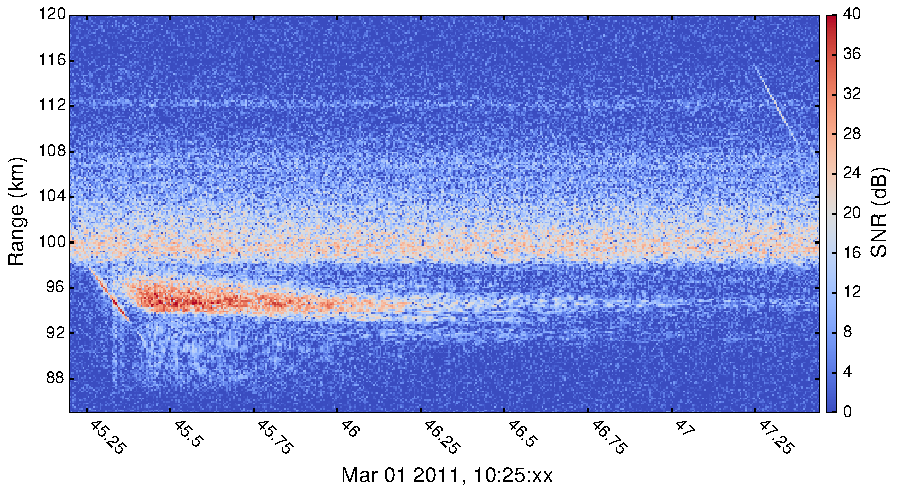
\includegraphics{equatorial_example_mf_rti_3}};
  \draw[green!80!black] (1.15,3.93) rectangle (13.95,4.74);
  \draw[purple] (1.4,2.8) rectangle (11.5,3.87);
  \draw[purple] (12.6,5.8) rectangle (13.7,7.4);
 \end{tikzpicture}
 \caption[The equatorial ionosphere as measured by the Jicamarca ISR]{\emph{The equatorial ionosphere as measured by the Jicamarca ISR.} Scattering due to the \textcolor{green!80!black}{equatorial electrojet} is seen in a narrow band around 100 km range (altitude). The other significant scattering is due to two \textcolor{purple}{meteors}.}
 \label{fig:electrojet_example}
\end{figure}%
It also is relatively stationary, and so it produces no Doppler frequency shift to complicate the scattered signal. Though the electrojet is important in its own right, it is often seen as clutter when trying to measure other ionospheric processes.

Another ubiquitous class of scatterers in the equatorial ionosphere and globally are meteors. When viewed by a high-power large-aperture (HPLA) radar like the ISRs, meteors exhibit two types of scattering: head echoes and trail echoes. Both are shown in Figure \ref{fig:meteor_scattering_example}.
\begin{figure}[tbp]
 \centering
 \begin{tikzpicture}[very thick]
  \node[above right] at (0,0) {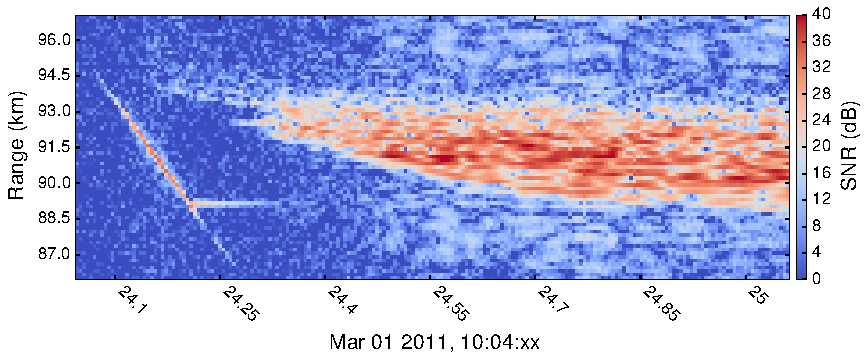
\includegraphics{head_and_flare_mf_rti_3}};
  \draw[purple] (2.7,5) -- (2.7,4.5) -- (8.5,2.6) -- (13.575,2.6) -- (13.575,5) -- cycle;
  \draw[green!80!black,shift={(2.9,3.5)},rotate=-55] (-2.15,-0.235) rectangle (2.15,0.235);
  \draw[yellow!80!black] (3.3,2.65) rectangle (5,3);
 \end{tikzpicture}
 \caption[Examples of meteor head and trail echoes]{\emph{Examples of meteor head and trail echoes.} Two types of meteor scattering are observed from the same meteor by the Jicamarca ISR. The \textcolor{green!80!black}{head echo} is the narrow streak on the left, while the \textcolor{purple}{non-specular trail echo} is the range-spread scattering on the right. The head echo also exhibits a \textcolor{yellow!80!black}{flare} with a sudden increase in signal strength and longer-lasting scattering at about 89 km range (altitude).}
 \label{fig:meteor_scattering_example}
\end{figure}%
A head echo represents scattering from the dense ball of plasma traveling with the meteoroid \autocite{CODD05}. In a radar signal intensity image plotted as range (or altitude) versus time (known as a range-time-intensity or RTI plot), head echoes appear as a narrow streak that descends in altitude with time. Because the meteoroid and head plasma are moving at high speed toward the radar as they descend in altitude, head echoes have a large positive Doppler frequency shift that complicates their measurement. Observing the head echo's speed, either by change in altitude or through the Doppler shift, allows one to determine the meteoroid's speed. If angular speed measurements are available through interferometry or monopulse, the full velocity and hence orbit of the meteoroid can be calculated. In addition, the signal strength and deceleration of the head echo can be used to determine the mass and density of the parent meteoroid \autocite{CVL+12}.

Once the meteor plasma is created by the meteoroid, it diffuses quickly into a trail that is left behind in the meteoroid's wake. Scattering from the trail can then happen either specularly or non-specularly. For specular scattering, the line of trail plasma acts like a mirror to reflect the radar signal \autocite{Sug64}; with a monostatic radar system where the transmitting and receiving antenna are one in the same, this means that the meteor trail must be perpendicular to the radar pointing direction in order for it to be seen specularly. Non-specular scattering is only possible when the radar points near perpendicularly to the Earth's magnetic field; turbulence sets up field-aligned irregularities of the trail plasma within a few tenths of seconds, providing enhanced scattering in the direction perpendicular to the magnetic field until the irregularities dissipate after a few seconds \autocite{DOCH02}. The example seen in Figure \ref{fig:meteor_scattering_example} is of a non-specular trail. Both types of trail echoes can be used to calculate meteoroid speed \autocite{CES97, DDC+04} and observe upper atmospheric winds \autocite{HFV01, OSS+09}.

\subsection{Challenges}
\label{intro_radar_challenges}
Much of what we know about the ionosphere has been gleaned from radar data, but there are still processes that are difficult to analyze. Radar presents an inherent conflict between sensitivity and ambiguity; longer transmitter pulses are needed to put more energy on target, but they have a correspondingly poorer range discrimination capability. Pulse compression, encoding the waveform on transmission and decoding the returned signal on reception using matched filtering, is the standard way to settle the conflict. However, matched filtering still results in ambiguity in the form of self-clutter \autocite{Woo80}. Because of this conflict, it is difficult to make high quality measurements in situations where both sensitivity and high resolution are needed.

With meteors, for example, we lack good observations of two phenomena: fragmentation and flares. In the case of fragmentation, \textcite{MBMC10} show meteor head echoes with an oscillating signal intensity that they explain by modeling the signal as interference between two separate scattering centers, with the theory that such a signal represents the result of meteoroid fragmentation. An example of this oscillation is shown in Figure \ref{fig:mathews_fragmentation}, but the fragmentation theory that could explain it has not been definitively proven.
\begin{figure}[tbp]
 \centering
 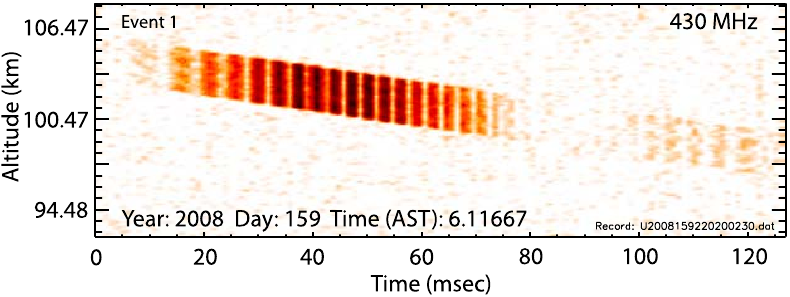
\includegraphics[width=0.75\textwidth]{mathews_fragmentation}
 \caption[Meteor head echo oscillations]{\emph{Meteor head echo oscillations.} This data from the Arecibo radar shows a meteor head echo with oscillating signal strength. The figure is reproduced from \textcite{MBMC10}, and unfortunately no color scale for the signal strength was given. \textcite{MBMC10} theorize that this oscillation indicates interference between two distinct head echo scatterers produced by meteoroid fragmentation.}
 \label{fig:mathews_fragmentation}
\end{figure}
Flares and the related terminal events are a process sometimes seen with head echoes where the signal intensity suddenly increases and trail scattering is immediately visible at the location of the event. An example of this process can be seen in Figure \ref{fig:meteor_scattering_example}, where a flare accompanies the meteor head echo. Currently no evidence has been observed that would explain why flares happen. Higher resolution data with reduced ambiguity is necessary to find answers to these mysteries, but such data cannot be produced with current techniques.

These challenges are somewhat unique to the applications found in the ionospheric radar community. Because of the wide variety of plasma processes and the corresponding demands on detail in space, time, and frequency, a wide variety of transmission waveforms are used. Some of these waveforms use deliberately-spread energy in frequency space to break the inherent relationship between sensitivity and resolution. Unfortunately, matched filter processing brings ambiguity and decoding artifacts, problems which cannot be ignored due to the high range of signal strength from one scatterer to the next. Current radar measurement techniques need to improve in four major areas to meet the challenges presented by the host of ionospheric plasma processes:
\begin{inparaenum}[1)]
 \item Differentiation of targets in crowded and variable environments, such as the ability to separate meteor and electrojet signals in the equatorial ionosphere;
 \item Elimination of self-interference of range-spread targets, which include non-specular meteor trails among others;
 \item Higher resolution to observe small-scale processes, such as meteoroid fragmentation and meteor flares; and
 \item Flexibility to achieve all of these goals at once.
\end{inparaenum}

\section{Sparsity}
\label{intro_sparsity}
The concept of sparsity is fundamental to how the brain processes information and manages to make sense of the deluge of sensory inputs that it receives. This principle, known as \emph{sparse coding}, states that "information is represented [in the brain] by a relatively small number of simultaneously active neurons out of a large population" \autocite{OF04}. Sparse coding makes the inherent structure of natural signals explicit, providing increased storage capacity and better energy efficiency in addition to simplifying higher-level reasoning. To achieve sparse coding, individual neurons respond to and represent just one particular aspect of a sensory input: an image is viewed through the retina, and a small number of neurons in the visual cortex respond to the image's localized patterns and edges \autocite{OF97}; a sound resonates at the individual frequencies of the inner ear hairs, and a sparse collection of neurons respond to the different frequency bands and corresponding time windows of the wave \autocite{Lew02}. The responses of the individual neurons collectively form a dictionary from which a small number of elements are used to represent any one particular input. Though this neurological example represents just one case of the practical use of sparsity, the concept of finding simple descriptions to represent and reason with information is universally applicable. In a philosophical sense, sparsity is embodied by the principle of Occam's Razor: the simplest explanation is best.

\subsection{Sparsity in Nature}
\label{intro_natural_sparsity}
As evident with the success of sparse coding in the brain, many natural phenomena have sparse representations, and great use can be made of this fact to perform compression in the digital domain. Mathematically, signals like images, sound waves, or radar returns can be represented with vectors. In the case of images, this can be as simple as dividing the image into a fixed number of pixels and having each vector element give the color and intensity value of a single pixel. If the vector representation is sparse, with only a few of its elements nonzero (or even approximately sparse with most elements \emph{close} to zero), then one can compress the signal by only storing the nonzero values (or values above a certain threshold).

But alas, the straightforward pixel representation of most images results in a vector that is dense with values, and this holds true for the straightforward representation of many other signals as well. As is the case in the brain, however, a sparse representation is often possible by choosing a dictionary of fundamental signals and composing any particular signal through combinations of the dictionary elements. If only a small number of the dictionary signals need to be used, then the vector giving the respective weights for a particular signal will be sparse. This is how images are processed in the visual cortex with a wavelet-like dictionary and how they are compressed in the JPEG format with a discrete cosine transform dictionary.

\begin{figure}[tbp]
 \centering
 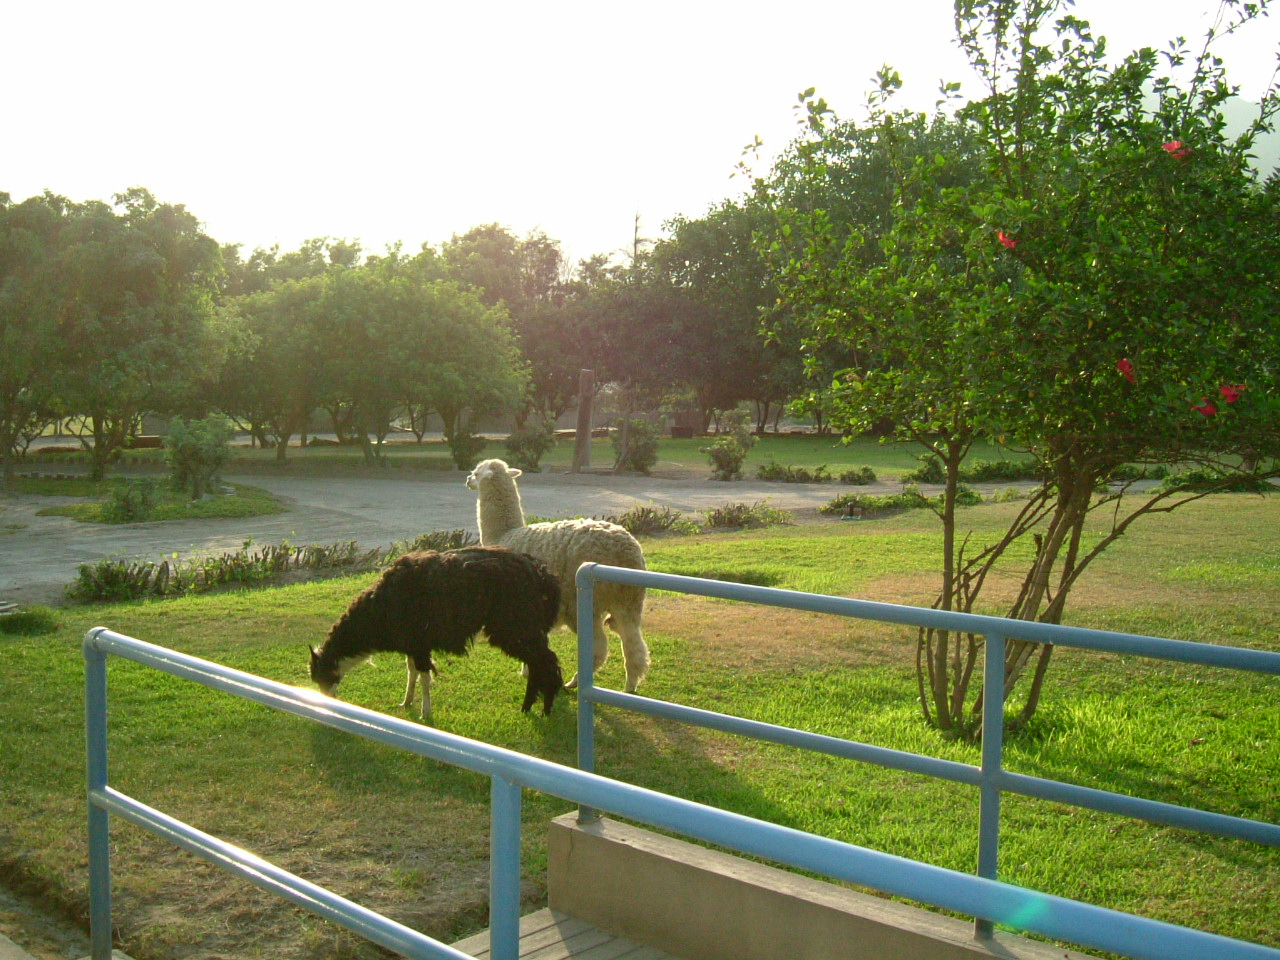
\includegraphics[width=0.6\textwidth]{jicamarca_alpacas}
 \caption[The structure of natural images]{\emph{The structure of natural images.} This digital image of alpacas at Jicamarca is 1280 $\times$ 960 pixels, and at 3 bytes per pixel it would require 3600 KiB of memory to store uncompressed. In its current JPEG compression format, it requires 420 KiB of memory instead. Structure in the image (patterns of color and continuity of edges) is used to reduce the required memory by a factor of about 8.5.}
 \label{fig:jicamarca_alpacas}
\end{figure}%
As a concrete example in the imaging case, consider Figure \ref{fig:jicamarca_alpacas}. Uncompressed, this picture of alpacas at the Jicamarca radar site requires 3600 KiB of memory to store, 1280 $\times$ 960 pixels at 3 bytes per pixel. When compressed in the JPEG format through a discrete cosine transform and by discarding unimportant (small) coefficients to create an exactly sparse representation, this image requires 420 KiB of memory. That's about an 8.5 times savings, representative of the structure inherent in the image and captured in the chosen dictionary.

\subsection{Sparsity in Radar}
\label{intro_radar_sparsity}
Radar signals are not exempt from the sparsity seen in nature. A radar transmits a signal and measures the intensity and phase of any reflections as a function of distance, with Doppler frequency shifts present in the reflection if a target is moving. Reflections from most radar scenes occupy only a small portion of that range-frequency space because the targets themselves are small in number and either spatially limited, have a compact Doppler spectrum from organized movement, or both. Most of the space being observed by the radar does not reflect any signal. Using a dictionary that decomposes signals on a joint range-frequency space captures the natural structure of radar targets and makes the sparsity exploitable.

\subsection{Sparsity in Action}
\label{intro_sparsity_research}
Whether influenced by research into brain physiology or not, the concept of sparsity has come to the fore in many fields of scientific research as a means of speeding, simplifying, or increasing the accuracy of information processing. Often this research falls under the moniker of \emph{compressed sensing}, which exploits sparsity, global measurement, and nonlinear reconstruction to acquire data faster or with higher resolution. Conceptually, since images are often sparse, it does not make sense to measure each pixel individually (as with a regular camera) only to then throw most of that data away to compress it. Instead, compressed sensing takes the approach of directly measuring a compressed representation of the image in order to save time and memory.

Applications of compressed sensing are continually increasing in number. Notable examples that span a variety of fields include the following: the single pixel camera, which uses a filter to randomly mix components of an image and produce a series of mixed-image single pixel readings from which the original image can be reconstructed \autocite{DDT+08}; compressed magnetic resonance imaging, which undersamples the spatial Fourier transform space of the image to speed acquisition and assumes image sparsity to achieve reconstruction \autocite{LDSP08}; and highly-parallel gene screening, which forms overlapping groups of genetic samples from a large set of donors, tests each group in bulk, and assumes rarity of the tracked gene pattern to determine which individual donors have it \autocite{EGB+10, GER12}. Sparsity serves as a useful representation of prior knowledge in all of these and many more applications, so it is no wonder that many fields of research have found success in leveraging sparsity to make important advances.

\section{Contributions}
\label{contributions}
In developing a sparsity-based radar technique for flexible, high-resolution measurement of ionospheric plasmas, this dissertation makes several important contributions:
\begin{itemize}
 \item \emph{A new perspective for radar measurements is espoused in which the radar scene reflectivity is recovered by inverting a mathematical model.}
 \begin{itemize}[]
  \item It is intuitively known that radar signals are sparse in a delay-frequency basis, but traditional approaches are not well-equipped to take advantage of that fact. A discrete radar model that captures signal sparsity is proposed using an image-blurring analogy, and this model is noted to be the adjoint of the standard pulse compression technique that uses a matched filter bank. Thanks to this connection between the two methods, an intuitive interpretation of the inversion technique as an iterative thresholding matched filter is presented.
 \end{itemize}
 \item \emph{A discrete radar model is rigorously derived from the continuous measurement equation for a general target scene.}
 \begin{itemize}[]
  \item The derivation results in an explicit formulation for how the discrete model's reflectivity coefficients represent arbitrary distributed scatterers. Using this expression, it is shown that true target sparsity is reasonably preserved in the discrete representation provided that the number of frequency grid points is high.
 \end{itemize}
 \item \emph{A novel waveform inversion technique is formulated based on finding a sparse representation of the radar scene using the discrete model.}
 \begin{itemize}[]
  \item Recovery of the true solution via $l_1$-norm minimization is proposed based on the theory of compressed sensing. This theory is leveraged to provide theoretical guarantees for the recovery of the true solution provided that the radar pulse waveform produces sufficiently incoherent measurements and that the number of measurements is at least on the order of the solution's sparsity. Waveform inversion is shown to eliminate matched filter sidelobe artifacts and enable higher-resolution solutions.
 \end{itemize}
 \item \emph{The waveform inversion method is implemented using modern convex optimization techniques tailored for efficient computation.}
 \begin{itemize}[]
  \item The focus is on algorithms based on the proximal operator because of their performance, ease of use, and ability to handle large problem dimensions. Since these algorithms are an active area of research, the implementation combines acceleration and adaptive step size enhancements from separate formulations to enable state-of-the-art convergence performance. All computer code is made freely available as open-source software to encourage further development, adoption, and collaboration.
 \end{itemize}
 \item \emph{The real-world flexibility and effectiveness of the inversion technique is demonstrated by the elimination of filtering artifacts from meteor observations made with a variety of standard radar waveforms.}
 \begin{itemize}[]
  \item Successful inversion is shown to depend on the compactness of the peak of the waveform's ambiguity function, while quality of the solution is shown to depend on the fidelity of the transmitted waveform to its idealized model. Increased resolution of the inversion solution is demonstrated but not validated, although the results are promising for future applications.
 \end{itemize}
\end{itemize}

\section{Reader's Guide}
\label{outline}
This dissertation is divided into four parts that build on one another but are relatively self-contained: introduction, radar analysis, waveform inversion, and conclusion. The preceding introduction is intended to familiarize the reader with the primary topics of interest in order to motivate and connect the work as a whole. Part \ref{part_radar_analysis} concerns radar analysis and goes into more detail about how radar measurements are made: Chapter \ref{radar_background} describes current waveform coding and processing techniques and discusses their limitations; Chapter \ref{radar_model} details the derivation and analysis of a mathematical radar model, providing a different way of analyzing radar measurements. The next segment, Part \ref{part_waveform_inversion}, introduces a waveform inversion method that combines the radar model with prior information of sparsity: Chapter \ref{sparsity_background} describes the theory of compressed sensing and related methods of convex optimization; Chapter \ref{waveform_inversion} details the implementation of the waveform inversion technique, including algorithmic advances; and Chapter \ref{experimental_results} provides experimental results using the Jicamarca radar to test waveform inversion and compare the effect of different waveforms. Finally, Part \ref{part_conclusion} contains the concluding chapter, which discusses the benefits provided by the new techniques and highlights areas for future research. One appendix is included, Appendix \ref{reflectivity_coefficients}, which details the simplification of the reflectivity coefficient expression derived in Chapter \ref{radar_model} as part of the radar model.

%The other two appendices cover techniques that are especially helpful for processing meteor data: Appendix \ref{clustering} describes a clustering approach that enables automatic detection and classification of radar signals; and Appendix \ref{super_resolution} describes the interpolated matched filter method used for super-resolution of range and range-rate estimates and analyzes its statistical accuracy via simulation.
\part{Radar Analysis}
\label{part_radar_analysis}
\graphicspath{{chapters/radar_background/figures/}}
\chapter{Radar Background}
\label{radar_background}
Radars come in a variety of forms, but for this work we are primarily concerned with pulsed monostatic radars. In this mode of operation, a radar transmits a pulse of electromagnetic energy and then switches to a listening mode to record the signal from any resulting reflections. The received power $P_r$ backscattered from a target is described by the radar equation \autocite{Sko01}:
\begin{equation}\label{eq:radar_equation}
 P_r = \frac{P_t G}{4\pi r^2} \times \sigma \times \frac{A_e}{4\pi r^2}.
\end{equation}
The transmitted power $P_t$ is concentrated by the antenna with a gain of $G$, but it also decays with distance (or range) $r$ according to $1/(4\pi r^2)$ as it spreads into space. The target then scatters a fraction of the power, the target's radar cross section $\sigma$, back toward the radar. The backscattered power once again decreases with range $r$ before returning to the antenna and experiencing a gain dependent on the effective aperture area $A_e$. In this monostatic case with the transmitting and receiving antenna co-located, the aperture is related to the transmitting gain by $G = 4\pi A_e/\lambda^2$, where $\lambda$ is the wavelength of the radio wave. Though it is important to remember how the received power relates to the radar's power and gain parameters ($P_t$, $G$, $A_e$) and the target's cross section and range ($\sigma$, $r$), we will mostly be able to ignore these effects by working only in terms of the received power as a function of range or, equivalently, time delay.

Once a pulse is sent and the received signal is recorded for as long as desired, the process is repeated to monitor how the radar targets change over time. The time from one pulse to the next is called the \emph{pulse period} and its inverse the \emph{pulse repetition frequency} (PRF). The PRF is an important parameter in the design of a radar experiment since it specifies the amount of time during which the radar can listen for reflections. Hence, it also gives the maximum unambiguous distance at which targets can be measured. For ionospheric experiments, pulse periods on the order of one to ten milliseconds, at a minimum, are common. With a zenith-pointing radar, one millisecond corresponds to a maximum unambiguous range of 150 km, which falls in the E-region (the total distance traveled by a returning wave in 1 ms is $c [m/s] * 1e^{-3} [s] \approx 300 [km]$ where $c \approx 3e8 [m/s]$ is the speed of light, so the maximum range is half that).

Usually these pulsed monostatic radars operate at a fixed frequency, or multiple fixed frequencies in independent channels. Data is typically acquired by sampling the received waveform so that its zero frequency corresponds to the radar's baseband frequency. This frequency shift is accomplished either directly in the digital domain after high-frequency sampling or with analog filtering and mixing \autocite{Ric05, Sko08}. Either way, the end result is a digitally sampled signal of complex numbers encoding the magnitude and phase of the received signal, a vector that can be stored and further analyzed to extract information about the radar scene. We employ the following notation for representing the transmitted and received radar signals: the transmitted waveform is represented by the complex sequence $s[l]$ with $L$ elements and indices $l=0,\dotsc,L-1$; the received waveform is represented by the complex sequence $y[m]$ with $M$ elements and indices $m=0,\dotsc,M-1$. For consistency, we will always use $l$ to index the transmitter sequence, $m$ to index the received sequence, and the corresponding capital letters to denote the respective sequence lengths.

\section{Pulse Design}
\label{pulse_design}
While design parameters like the pulse period and system parameters like the transmitter power and antenna gain are important in designing a radar experiment, the pulse itself is critical. Imagine the pulse as a square wave centered at the radar's operating frequency as shown in Figure \ref{fig:pulse_returns}. In this figure, the delay space is divided into samples according to the sampling period, and the transmitted and received waveforms are shown along with their vector counterparts. The waveforms display a fixed frequency, the radar operating frequency, but are modulated on and off according to the pulse length. Although the ideal on/off of a square wave is never achieved in practice, it is a convenient way to conceptualize the waveforms.
\begin{figure}[tpb]
 \centering
 \begin{subfigure}{0.5\textwidth}
  \centering
  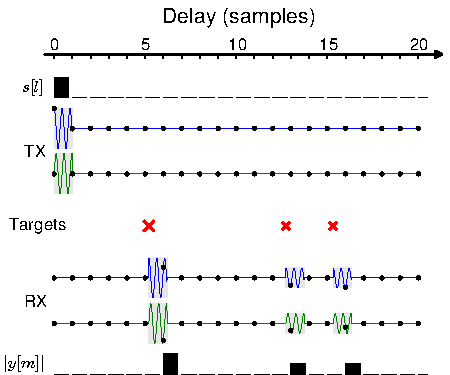
\includegraphics{shortpulse_return}
  \caption{Short pulse}
  \label{fig:short_pulse_return}
 \end{subfigure}%
 \begin{subfigure}{0.5\textwidth}
  \centering
  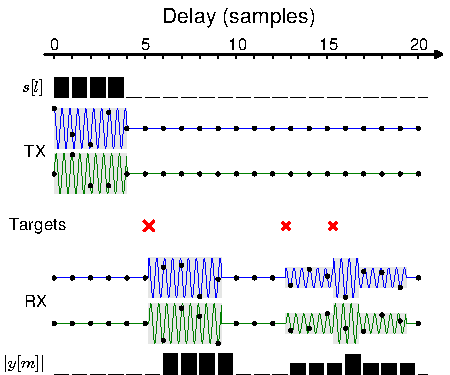
\includegraphics{longpulse_return}
  \caption{Long pulse}
  \label{fig:long_pulse_return}
 \end{subfigure}
 \caption[Transmitted and received signals for a short and long pulse]{\emph{Transmitted and received signals for a short and long pulse.} In each case, transmitted (TX) and received (RX) waveforms are shown as a function of delay along with the corresponding sampled baseband signals $s[l]$ and $y[m]$. Each waveform has an in-phase (blue) and quadrature (green) component, representing the wave's magnitude and phase when thought of as the real and imaginary parts of the complex signal. The received waveform encapsulates the delays and magnitude differences applied to the transmitted pulse by three point targets. Because of ambiguity created by the pulse length, the received signal for the short pulse is easier to interpret than for the long pulse, but the long pulse allows for increased total power through averaging over multiple samples.}
 \label{fig:pulse_returns}
\end{figure}%

\subsection{Pulse Length}
The simplest mode of operation matches the length of the transmitted pulse with the sampling rate of the received signal. In this way, each sample represents the sum of reflections over a particular range window with width corresponding to the pulse length. This short pulse mode of operation is depicted in Figure \ref{fig:short_pulse_return}, where three point targets appear individually as three nonzero samples in the received signal. In general, range resolution is defined by the sampling rate, while range ambiguity, or the interference region for multiple scatterers, is defined by the pulse length. In the short pulse case, the range resolution matches the range ambiguity so that the ambiguity does not pose an interpretation problem.

The primary downside of a short pulse is that it limits the sensitivity of the radar in terms of energy on target. Since the peak power of a pulse is limited by the physical radar equipment, the only way to increase the total power is to increase the pulse length. With a pulse greater than the sampling period, one can add the returned signal over multiple samples within the pulse to achieve a higher sensitivity due to higher total power. However, a longer pulse also increases the range ambiguity of the measurement since the return from any single target will affect multiple receiver samples. This long-pulse mode of operation is depicted in Figure \ref{fig:long_pulse_return}. The example shows both the positives and negatives of a longer pulse: more samples for increased sensitivity with the first target, but ambiguity in the received signal between the latter two closely-spaced targets.

Two additional points are relevant when discussing pulse length: transmitter duty cycle and Fourier frequency resolution. In order to transmit large amounts of power instantaneously, transmitters often have a maximum duty cycle that describes the fraction of time that the transmitter is allowed to be on. A duty cycle is necessary so that there is enough off time to build up the power supply and allow physical components to cool. Because of these requirements, the pulse length cannot be increased indiscriminately and has a fixed limit with respect to the pulse period. The other consideration is Fourier frequency resolution. For persistent targets, pulse-to-pulse Fourier analysis is possible to measure how the target evolves in time, with the maximum observable frequency component given by half the pulse repetition frequency. For quickly-evolving or transient targets, the pulse-to-pulse method of Fourier analysis is not sufficient and intra-pulse Fourier analysis is necessary. In that case, the maximum observable frequency is half the sampling frequency and the resolution is the inverse of the pulse length. Thus, increasing the pulse length also has the benefit of improving the frequency resolution of intra-pulse Fourier analysis.

\subsection{Pulse Waveforms}
One way to deal with the ambiguity problem is to code the pulse by modulating it with a designed waveform. Because of the way that coding allows for concentration of the pulse energy after decoding, this process is often called \emph{pulse compression}. One simple and widespread method is linear frequency modulation (LFM), also known as a chirp waveform. A chirp pulse starts off at a low frequency and linearly increases in frequency over time to a high frequency, or vice-versa. An example is given in Figure \ref{fig:lfm_chirp}.
\begin{figure}[tpb]
 \centering
 \begin{subfigure}{\textwidth}
  \centering
  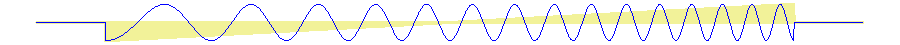
\includegraphics{lfmpulse}
  \caption{LFM Chirp}
  \label{fig:lfm_chirp}
 \end{subfigure}
 
 \vspace{\baselineskip}
 \begin{subfigure}{\textwidth}
  \centering
  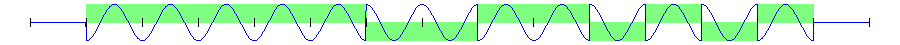
\includegraphics{barker13pulse}
  \caption{Barker-13}
  \label{fig:barker13_pulse}
 \end{subfigure}
 
 \vspace{\baselineskip}
 \begin{subfigure}{\textwidth}
  \centering
  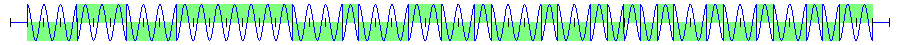
\includegraphics{mslpulse}
  \caption{Minimum peak sidelobe (51 bauds)}
  \label{fig:msl_pulse}
 \end{subfigure}
 \caption[Waveform encoding examples]{\emph{Waveform encoding examples.} These pulse waveforms depict three commonly used encodings: \textbf{(\subref{fig:lfm_chirp})} an LFM chirp pulse with a linear frequency sweep from low to high, \textbf{(\subref{fig:barker13_pulse})} a binary phase-coded pulse using the Barker-13 code, and \textbf{(\subref{fig:msl_pulse})} a binary phase-coded pulse using a minimum peak sidelobe code with 51 bauds. The yellow fill in the background of \textbf{(\subref{fig:lfm_chirp})} indicates the pulse's frequency with respect to the baseband, while the green rectangles in \textbf{(\subref{fig:barker13_pulse})} and \textbf{(\subref{fig:msl_pulse})} indicate the positive or negative phase of each baud.}
 \label{fig:waveform_encodings}
\end{figure}%
Another common form of modulation is to divide the pulse into equal length segments called \emph{bauds} and encode using the phase of each baud. Often the codes use only two opposite phases (e.g. $1$ and $-1$) and the process is called binary phase coding, but the use of more phases is certainly possible. Two examples of commonly-used and well-behaved binary phase codes are shown in Figure \ref{fig:waveform_encodings}. The Barker-13 code of Figure \ref{fig:barker13_pulse} has 13 bauds with phases described by the binary sequence
\begin{equation}
 s_{\text{B}_\text{13}} = 1111100110101,
\end{equation}
while the minimum peak sidelobe code of Figure \ref{fig:msl_pulse} has 51 bauds with phases described by the binary sequence
\begin{equation}
 s_{\text{MSL}_\text{51}} = 000111000111111100010001100100010010101001001001011.
\end{equation}

\section{Matched Filtering}
\label{matched_filtering}
When coded pulses are used, or even just long pulses, one needs a way to decode the received result and integrate the distributed power. The intuitive way of doing this, by starting with each sample in the received signal and operating over a window the length of the pulse to reverse the effects of the code and sum the result, is called a \emph{matched filter}. Stated another way, the matched filter correlates every segment of the received signal with the transmitted pulse. Mathematically, the matched filter performs the correlation
\begin{align}
 u[p] &= \sum_{m=0}^{M-1} s^*[m - p + (L-1)] y[m]
 \intertext{or equivalently}
 u[p] &= \sum_{l=0}^{L-1} s^*[l] y[p + l - (L-1)],
\end{align}
where $s^*$ signifies the complex conjugate of the code $s$ and the matched filter result is denoted by $u[p]$ for $p=0,\ldots,P-1$ with $P=M+L-1$. These equations reference "out of bounds" indices of $y[m]$ and $s^*[l]$; for simplicity we take the convention that any out of bounds values are zero. The correlation process of the matched filter is shown in Figure \ref{fig:barker13_autocorrelation} in the context of autocorrelation of the Barker-13 code, which corresponds to the ideal case when the received signal is due to perfect reflection from a point target.
\begin{figure}[ptb]
 \centering
 \begin{tabular}{cc}
  $p=0$ & \raisebox{-0.5\height}{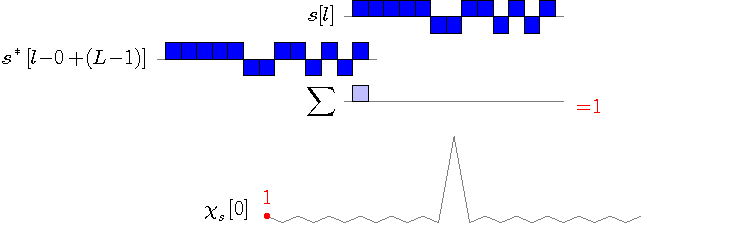
\includegraphics{autocorrelation_b13_0}}\\[\dimexpr-\baselineskip]
  \hline\\
  $p=1$ & \raisebox{-0.5\height}{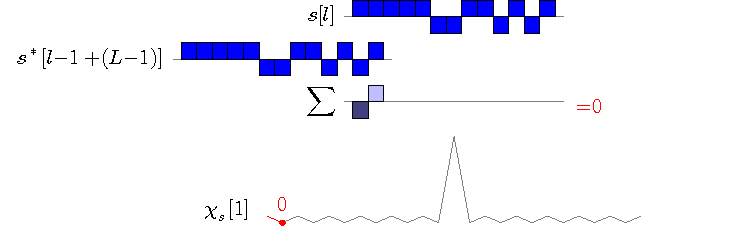
\includegraphics{autocorrelation_b13_1}}\\
  \hline\\
  $p=6$ & \raisebox{-0.5\height}{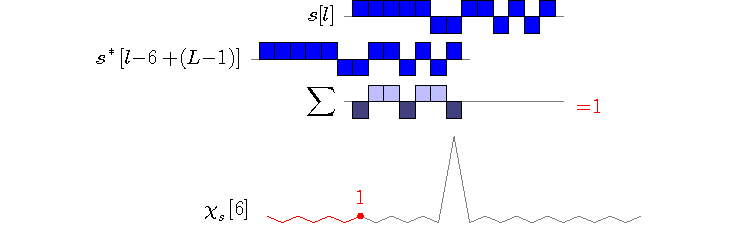
\includegraphics{autocorrelation_b13_6}}\\
  \hline\\
  $p=12$ & \raisebox{-0.5\height}{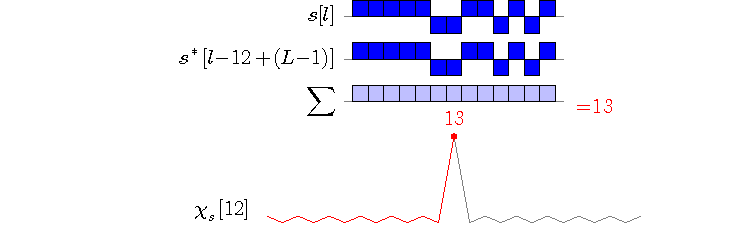
\includegraphics{autocorrelation_b13_12}}
 \end{tabular}
 \caption[Autocorrelation of the Barker-13 code]{\emph{Autocorrelation of the Barker-13 code.} Each panel depicts the calculation of a single sample $p$ for the autocorrelation of the Barker-13 code. The first two lines of each panel show the code sequence $s[l]$ and its shifted conjugate. The third line shows the resulting multiplication of the first two lines and sum total of the values. The fourth line gives a plot of the autocorrelation, highlighting the calculated sample.}
 \label{fig:barker13_autocorrelation}
\end{figure}%
The benefits of the matched filter are its sensitivity and ease of computation: it produces the optimal signal-to-noise ratio (SNR) when decoding point targets and takes the form of a simple linear filter.

There is one degree of freedom when computing the matched filter: one can scale the code $s$ by any amount and still have optimal SNR at the output. This is because increasing $s$ by a scalar quantity not only increases the magnitude of the output when run against a matching sequence, but it also equally increases the magnitude of the output when run against non-matching random noise. Since the output is typically examined in terms of SNR, this arbitrary scaling makes no difference to the analysis. In a practical sense, however, it is often convenient to scale the code $s$ so that it has an $l_2$ norm of one:
\begin{equation}\label{eq:scaled_code}
 s'[l] = \frac{s[l]}{\sqrt{\sum_{k=0}^{L-1} \abs{s[k]}^2}}.
\end{equation}
When this is done, noise at the output of the matched filter has the same average power as noise at the input, and no recalculation of the noise power is necessary to compute SNR.

\subsection{Autocorrelation and Range Sidelobes}
Since targets essentially reflect the transmitted signal, just with phase and power differences and mixing from multiple or distributed targets, we can examine the effect of matched filtering by looking at a code's autocorrelation:
\begin{equation}
 \chi_s[p] = \sum_{l=0}^{L-1} s[l] s^*[l - p + (L-1)],
\end{equation}
where $p=0,\ldots,P-1$ with $P=2L-1$. As shown in Figure \ref{fig:barker13_autocorrelation} for the Barker-13 code, the autocorrelation of any code has a peak in the middle, corresponding to when the received and transmitted codes are perfectly aligned. In the matched filter result, the peak occurs at the delay, or range, corresponding to the location of the reflecting target. Away from the peak, the autocorrelation is not zero but rather some pattern of varying response that depends on the code. When these off-peak responses are seen in the matched filter result, they are called \emph{range sidelobes}.

Particular codes are selected for use because of their autocorrelation properties, where keeping sidelobe response to a minimum is desirable to minimize ambiguity and artifacts. The Barker-13 code is the longest in a class of Barker codes of differing lengths that have a maximum sidelobe level of one. It is possible to enforce similar minimum peak sidelobe performance for codes of other (particularly longer) lengths; these are unsurprisingly called minimum peak sidelobe codes, and they have been found through simple brute force search \autocite{Lin75,CFB90,CHC01,CR05}. The 51-baud example given in Figure \ref{fig:msl_pulse} is just one of the codes of different lengths with the minimum peak sidelobe property. The LFM chirp that we encountered earlier also has well-behaved range sidelobes, and in that case they decay from the peak according to a sinc function.

\subsection{Frequency Banks of Matched Filters}
Moving targets complicate the use of a matched filter to decode the received signal because the Doppler frequency shift causes a mismatch. If a target is moving toward (away from) the radar, the reflected signal is shifted up (down) in frequency. In order to correlate properly, the matched filter needs to be similarly frequency shifted. Of course, the true frequency shift due to target motion is not known ahead of time, so it is another unknown that must be determined along with the target's range. We cope with this problem by processing the received signal with a bank of filters, each with a different frequency shift. Computationally, it is convenient to have these filters be equally spaced in frequency up to the maximum detectable frequency shift, determined from the sample rate according to the Nyquist criterion. When that is done, the filter bank can be computed efficiently through the Discrete Fourier Transform (DFT). The equation describing the matched filter bank is similar to the single matched filter:
\begin{align}
 u[n,p] &= \sum_{m=0}^{M-1} s^*[m - p + L-1]\, e^{-2\pi i n (m-p+L-1)/N}\, y[m]\\
 \intertext{or equivalently}
 u[n,p] &= \sum_{l=0}^{L-1} s^*[l]\, e^{-2\pi i n l / N}\, y[p + l - (L-1)].
\end{align}
The difference, of course, is that for each of the $N$ frequencies indexed by $n$ for $0,\dotsc,N-1$, the transmitted code is modulated at that frequency before correlation with the received signal.

Visualizing the results of a filter bank also poses a challenge. Since we will frequently have to deal with this type of visualization, a brief discussion is in order. Often we want to plot data from multiple pulses in order to see how the targets vary over time. With a filter bank, that means plotting signal strength as a function of three variables: range, frequency, and time. A natural representation is a video, with each frame being a plot of signal strength as a function of range versus frequency for a single pulse. Of course, that has the distinct disadvantage of not working well in print. A more suitable approach is to truncate one of the dimensions in some way. If all of the targets have a negligible or similar Doppler shift, then it is reasonable to just plot the data for that one frequency. This results in a standard range-time-intensity (RTI) plot with range as the vertical axis, pulse time as the horizontal axis, and signal intensity represented by color or shading. Figure \ref{fig:electrojet_example} in the introduction is an example of this approach. However, when moving and stationary targets mix (as with the meteor head echo and trail shown in Figure \ref{fig:meteor_scattering_example}), single frequency truncation is insufficient. In those cases and when an RTI-type plot is desired, the single frequency that gives the maximum response over all ranges is selected for each pulse individually. Most of the time this is sufficient to produce a well-decoded plot, but it still fails when multiple frequency-shifted targets appear in the same pulse. There are other approaches for visualizing filter bank outputs, but here we will only employ the peak-frequency-response approach for RTI plots.

\section{Measurement Ambiguity}
\label{radar_ambiguity}
When analyzing the received radar signal for a single pulse, we are interested in how the transmitted signal was reflected as a function of delay (range) and frequency (range-rate). A frequency bank of matched filters produces a peak response at the delay and frequency of any target, but it also produces off-peak sidelobes as an artifact of the filtering process. The delay-frequency sidelobes can, depending on their magnitude, obscure weaker targets or bias the measurement through interference. We call these effects measurement ambiguity.

\subsection{Ambiguity Function}
As we saw in the single matched filter case, sidelobes are a consequence of the autocorrelation of a particular code. The same is true in the filter bank case, except we must consider the autocorrelation not only as a function of delay but as a function of frequency:
\begin{multline}
 \chi_s[n,p;n',p'] = \sum_{m=0}^{M-1} s[m - p' + L - 1]\, e^{2\pi i n' (m-p'+L-1)/N}\\
 \times s^*[m - p + L - 1]\, e^{-2\pi i n (m-p+L-1)/N}.
\end{multline}
It is necessary to explicitly write this function in terms of the two frequency indices $n$ and $n'$ and the two delay indices $p$ and $p'$ because of the nonlinear interaction between frequency and delay in the exponential term. As with before, $n,n' \in [0, N-1]$, $p,p' \in [0, P-1]$, and $M = P - (L-1)$. The delay-frequency autocorrelation of a code is also known as its \emph{ambiguity function}, although this term is sometimes used to denote the squared magnitude of the autocorrelation \autocite{Woo80}. The sidelobes of a code are completely described by the code's ambiguity function.

To make this concept more accessible, consider again the example codes encountered earlier. The ambiguity functions of the Barker-13, minimum sidelobe, and LFM chirp waveforms are shown in Figure \ref{fig:ambiguity_functions}.
\begin{figure}[tpb]
 \centering
 \begin{subfigure}{0.5\textwidth}
  \centering
  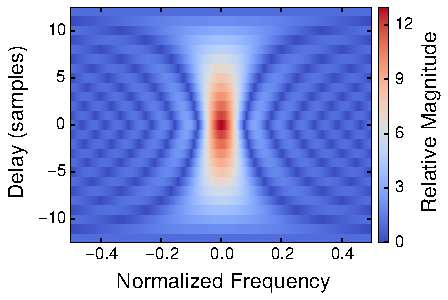
\includegraphics{ambiguity_uncoded}
  \caption{Uncoded pulse (13 samples long)}
  \label{fig:uncoded_ambiguity}
 \end{subfigure}%
 \begin{subfigure}{0.5\textwidth}
  \centering
  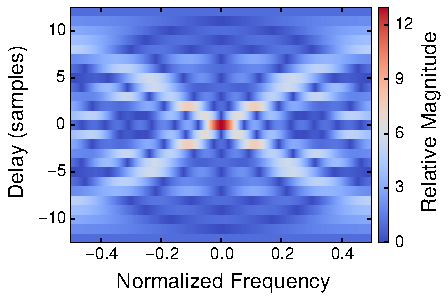
\includegraphics{ambiguity_barker13}
  \caption{Barker-13}
  \label{fig:barker13_ambiguity}
 \end{subfigure}
 
 \vspace{\baselineskip}
 \begin{subfigure}{0.5\textwidth}
  \centering
  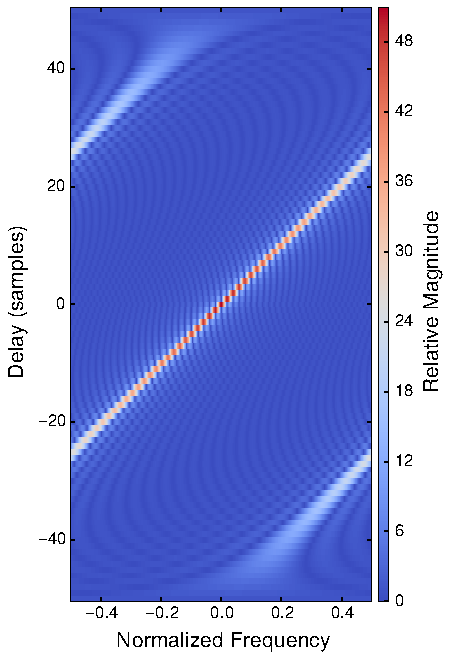
\includegraphics{ambiguity_lfm}
  \caption{LFM chirp (51 samples long)}
  \label{fig:lfm_ambiguity}
 \end{subfigure}%
 \begin{subfigure}{0.5\textwidth}
  \centering
  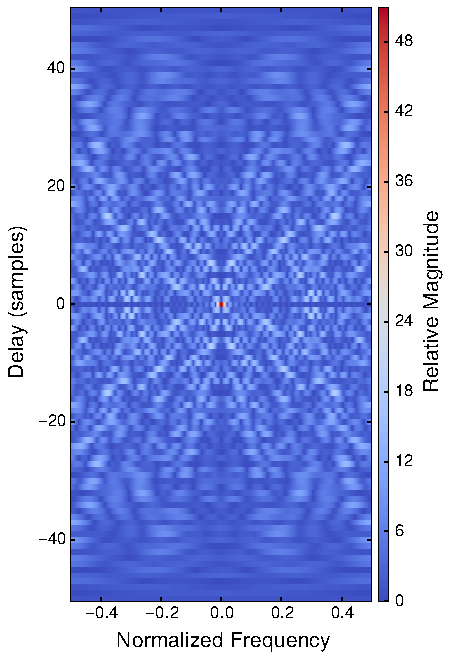
\includegraphics{ambiguity_msl}
  \caption{Minimum sidelobe (51 bauds)}
  \label{fig:msl_ambiguity}
 \end{subfigure}
 \caption[Ambiguity function examples]{\emph{Ambiguity function examples.} These delay-frequency images show the ambiguity function magnitude with $N=512$ frequencies for the \textbf{(\subref{fig:uncoded_ambiguity})} 13-sample uncoded pulse, \textbf{(\subref{fig:barker13_ambiguity})} Barker-13 code, \textbf{(\subref{fig:lfm_ambiguity})} 51-sample discretized LFM chirp with bandwidth equal to the sampling frequency, and \textbf{(\subref{fig:msl_ambiguity})} 51-baud minimum peak sidelobe code.}
 \label{fig:ambiguity_functions}
\end{figure}%
As a point of comparison, this figure also includes the ambiguity function of an uncoded pulse. All of the ambiguity functions have a peak centered at at zero delay and zero frequency, or rather the reflecting target's delay and frequency. The uncoded pulse has a strong response for many samples surrounding the peak: along the zero-frequency axis, the response decays linearly on both sides of the peak, while along the zero-delay axis, the response decays with the periodic sinc function. In contrast, the peaks for the Barker-13 and minimum sidelobe codes are well-defined and isolated with the sidelobe response lower but spread out across the delay-frequency space. The LFM chirp is interesting because of its ridge-like response, with strong ambiguity along a line in delay-frequency space but minimal sidelobes elsewhere. Thus, the LFM chirp is popular for use with a single matched filter since it is insensitive to frequency shifts (aside from a corresponding shift in the apparent target range).

\subsection{Sidelobes in Action}
The differences in ambiguity between these codes have a large impact in practice. Figures \ref{fig:meteor_uncoded_barker13} and \ref{fig:meteor_msl_lfm} show a meteor head echo and trail measured separately using the 50 MHz Jicamarca radar with a 40$\mu$s uncoded pulse, a 13$\mu$s Barker-13 pulse, a 51$\mu$s minimum sidelobe pulse with 51 bauds, and a 51$\mu$s LFM chirp with 1 MHz frequency sweep.
\begin{figure}[tpb]
 \begin{subfigure}{\textwidth}
  \centering
  \textsf{\footnotesize Mar 01 2011, 10:04:xx (s)}
  
  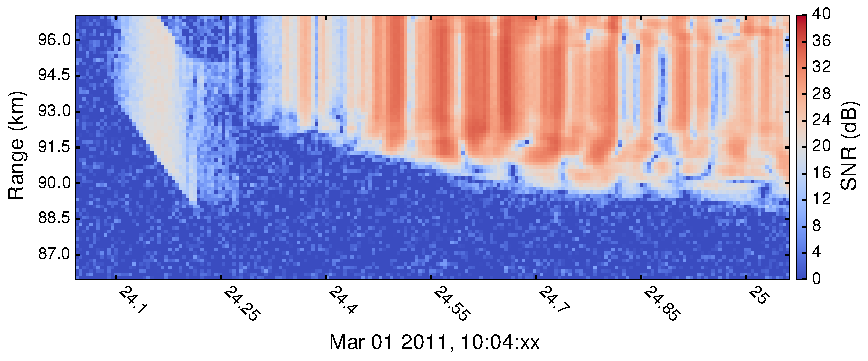
\includegraphics[trim=0px 20px 0px 3px,clip]{head_and_flare_rti_2}
  \caption{Uncoded pulse (40$\mu$s), unfiltered}
  \label{fig:meteor_uncoded_unfiltered}
 \end{subfigure}
 
 \vspace{0.5\baselineskip}
 \begin{subfigure}{\textwidth}
  \centering
  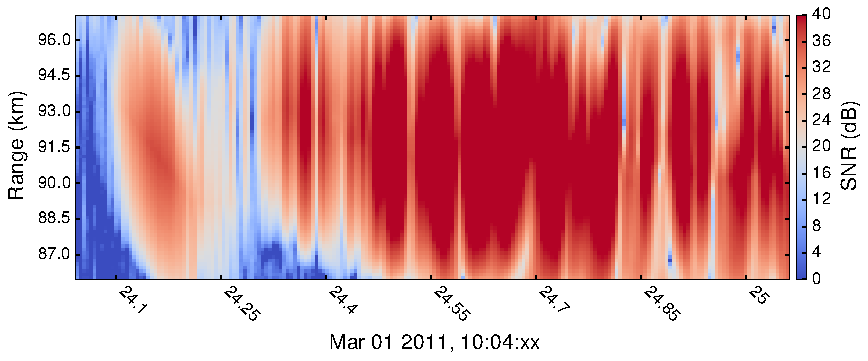
\includegraphics[trim=0px 20px 0px 3px,clip]{head_and_flare_mf_rti_2}
  \caption{Uncoded pulse (40$\mu$s), matched filter}
  \label{fig:meteor_uncoded_mf}
 \end{subfigure}
 \caption[Meteor head and trail measured with an uncoded pulse]{\emph{Meteor head and trail measured with an uncoded pulse.} These figures show the signal-to-noise ratio (SNR) as a function of range and time for one second of 1$\mu$s-sampled data taken with the 50 MHz Jicamarca radar. An uncoded pulse was used, with \textbf{(\subref{fig:meteor_uncoded_unfiltered})} showing the unfiltered result and \textbf{(\subref{fig:meteor_uncoded_mf})} showing the peak-frequency-response matched filter result. The SNR is low before filtering, but the range sidelobes resulting from the filter completely obscure the meteor trail.}
 \label{fig:meteor_uncoded_barker13}
\end{figure}%
\begin{figure}[tpb]
 \vspace{-1.5\baselineskip}
 \begin{subfigure}{\textwidth}
  \centering
  \textsf{\footnotesize Mar 01 2011, 10:04:xx (s)}
  
  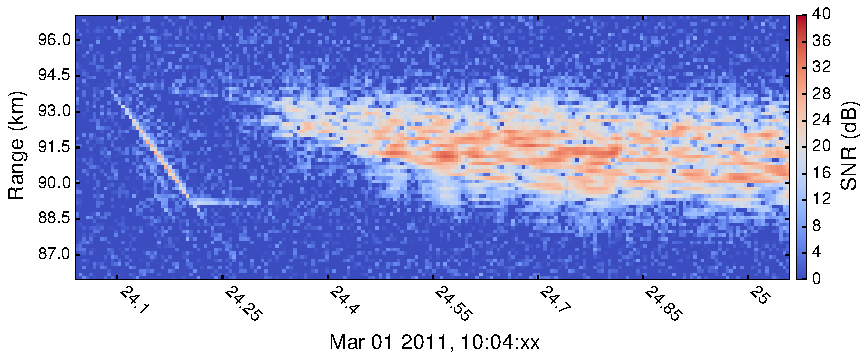
\includegraphics[trim=0px 20px 0px 3px,clip]{head_and_flare_mf_rti_0}
  \caption{Barker-13 pulse (13$\mu$s)}
  \label{fig:meteor_barker13_mf}
 \end{subfigure}
 
 \vspace{0.5\baselineskip}
 \begin{subfigure}{\textwidth}
  \centering
  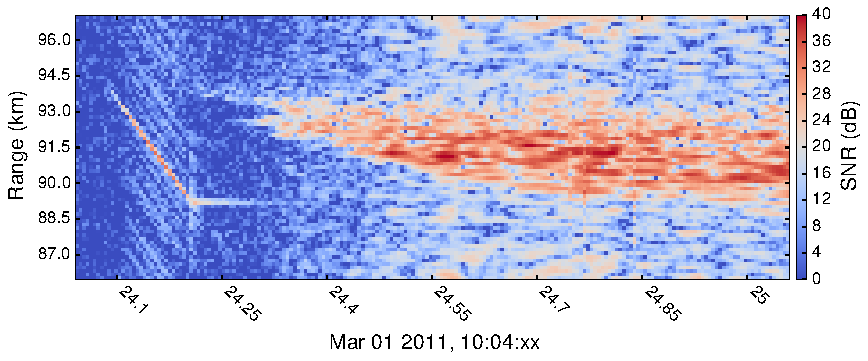
\includegraphics[trim=0px 20px 0px 3px,clip]{head_and_flare_mf_rti_1}
  \caption{Minimum peak sidelobe pulse (51$\mu$s with 51 bauds)}
  \label{fig:meteor_msl_mf}
 \end{subfigure}
 
 \vspace{0.5\baselineskip}
 \begin{subfigure}{\textwidth}
  \centering
  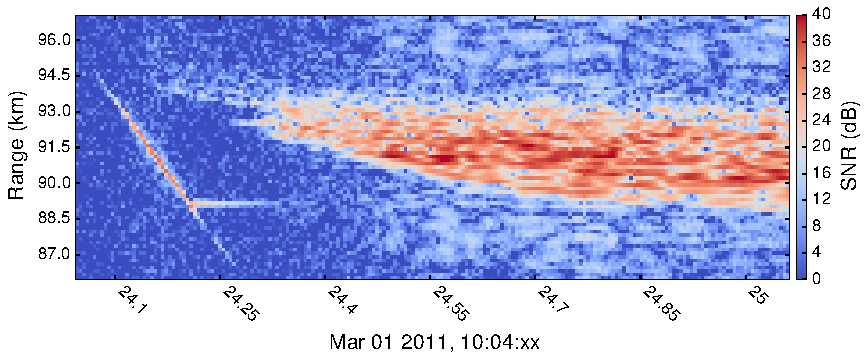
\includegraphics[trim=0px 20px 0px 3px,clip]{head_and_flare_mf_rti_3}
  \caption{LFM chirp (51$\mu$s with 1 MHz frequency sweep)}
  \label{fig:meteor_lfm_mf}
 \end{subfigure}
 \caption[Meteor head and trail measured with coded pulses]{\emph{Meteor head and trail measured with coded pulses.} These figures show the peak-frequency-response matched filter results for different waveforms over one second of 1$\mu$s-sampled data taken with the 50 MHz Jicamarca radar. Range sidelobes from the codes create significant ambiguity and make interpretation difficult.}
 \label{fig:meteor_msl_lfm}
\end{figure}%
Since these are RTI plots, the matched filter results show the peak-frequency-response filter for each pulse. Because of that, the artifacts that crowd the plot are mostly the zero-frequency-axis range sidelobes for each code. Unsurprisingly, the uncoded pulse's sidelobes completely dominate the output when that code is used. The meteor trail in particular appears as a high SNR mess. The Barker-13 code produces much more manageable sidelobes where the head echo and primary regions of trail scatter are clearly visible. Unfortunately, the Barker-13 pulse is necessarily much shorter in length, and the reduced sensitivity is evident with lower overall SNR. The minimum sidelobe code has higher SNR while keeping the acceptable sidelobe performance of the Barker-13 code. However, the sidelobes are still clearly significant and can easily obscure weaker scatterers, especially when the scatterers are shifted in frequency and have to contend with the very significant off-axis sidelobes. Finally, the LFM chirp produces the cleanest-looking results, an outcome which is not surprising given its ambiguity function. It is important to note though that they come at the cost of range bias and loss of frequency information; those shortcomings are only mitigated in this instance by the use of the other codes to determine the proper decoding frequency.

The example meteor head echo and trail are particularly well-behaved because they occur separately and without any other targets interfering. Even though that is usually the case when only meteors are observed, sidelobes are the primary reason that many outstanding ionospheric science questions cannot be satisfactorily answered with current techniques. Any time multiple or distributed scatterers are observed, sidelobes obscure or bias the measurements. The prior examples of challenging meteor phenomena, flaring in Figure \ref{fig:meteor_scattering_example} and fragmentation in Figure \ref{fig:mathews_fragmentation}, are just two important cases. Matched filtering is one way to decode coded radar measurements, and its limitations are clear. What is needed is a new decoding technique that keeps the benefits of the matched filter, sensitivity and efficient computation, but does not produce sidelobes. The problem in developing such a technique is that there are an infinite number of ways to construct a delay-frequency target scene that matches the measurements, and we're looking for the one that is both correct and sidelobe-free.

\section{Current Techniques}
\label{current_radar_techniques}
\subsection{Sidelobe Mitigation}
Accounting for matched filter ambiguity is not a new problem, and there are many ways it has been addressed in the past. The most obvious method is the one we've already covered: sidelobe mitigation through the selection of well-behaved codes. Obviously waveforms like the Barker codes, minimum peak sidelobe codes, and LFM chirp have more manageable sidelobes than an uncoded pulse or even most other waveforms. This is by design, as those codes were formulated to have either the minimum peak range sidelobes or to be insensitive to frequency shifts. Their typical use in applications such as satellite tracking, where sensitivity is essential and point-like targets are the norm, demonstrates their effectiveness in particular circumstances. As we've seen, though, these codes are only effective when it is simple to ignore the sidelobes that do remain. It is especially hard to ignore those sidelobes when targets with multiple Doppler frequency shifts are present, since the off-zero-axis delay-frequency sidelobes are quite significant. This is a consequence of the codes being designed to minimize only the zero-frequency-axis range sidelobes. Codes employing a larger set of phases, such as quadriphase codes \autocite{DLOV08}, show promise in improving performance over the widespread binary-phase codes \autocite{VLR+13}, but they still have many of the same fundamental sidelobe limitations.

\subsection{Alternating Codes}
Alternating codes are an approach to completely removing sidelobes by using a complementary set of codes over multiple pulses \autocite{LH87,Sul93,MVM08}. When the multi-pulse data is summed together, sidelobes from the individual codes cancel out to make the set sidelobe-free. Since incoherent scatter radars must already integrate over multiple pulses to get significant signal, alternating codes are widely used to measure incoherent scatter from the background ionosphere. As that application alludes to, alternating codes are an effective approach when target properties remain stationary over the time it takes to transmit the code set. Unfortunately, that is a constraint that limits flexibility and rules out many cases of interest.

\subsection{Inverse Filters}
It is also possible to leave matched filters behind altogether and use an alternative filtering or inversion technique. An inverse filter is one designed specifically to produce no range sidelobes at a point target's particularly frequency shift. Theoretically, inverse filters are infinite in length, but practically, finite-length truncation can achieve nearly indistinguishable inversion behavior. Like the matched filter, the inverse filter is a function of the transmitted code and is performed by a simple linear filtering operation on the received radar data. Since they are not optimal-SNR matched filters, however, inverse filters result in a loss of sensitivity that depends on the particular code used. Recent work into so-called perfect codes \autocite{LDPO09} make inverse filters more attractive, since perfect codes are designed so that the inverse filter is also the matched filter. One reason that perfect codes are not more widespread is that they require amplitude modulation in addition to phase modulation for each baud, and this can be difficult to achieve in practice.

Another reason that perfect codes are not more widespread is that inverse filters still produce significant sidelobes when the target frequency does not match the decoding frequency. This is evident in Figure \ref{fig:inverse_ambiguity_comparison}, which compares the ambiguity function for the Barker-13 code for both the matched filter and the inverse filter.
\begin{figure}[tpb]
 \centering
 \begin{subfigure}{0.5\textwidth}
  \centering
  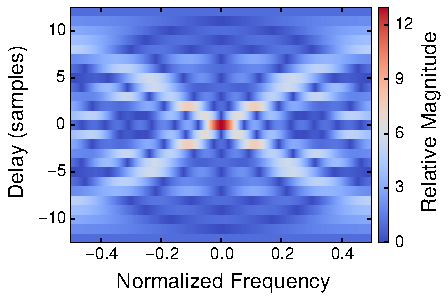
\includegraphics{ambiguity_barker13}
  \caption{Barker-13 matched filter ambiguity}
  \label{fig:barker13_matched_ambiguity}
 \end{subfigure}%
 \begin{subfigure}{0.5\textwidth}
  \centering
  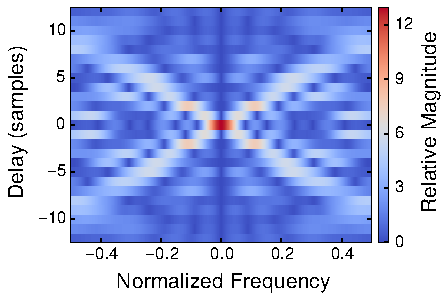
\includegraphics{ambiguity_inverse_barker13}
  \caption{Barker-13 inverse filter ambiguity}
  \label{fig:barker13_inverse_ambiguity}
 \end{subfigure}
 \caption[Comparison of matched and inverse filter ambiguity functions]{\emph{Comparison of matched and inverse filter ambiguity functions.} These delay-frequency images show the ambiguity function magnitude with $N=512$ frequencies for the Barker-13 code. The \textbf{(\subref{fig:barker13_matched_ambiguity})} matched filter and \textbf{(\subref{fig:barker13_inverse_ambiguity})} inverse filter ambiguities are nearly identical apart from the zero-frequency axis, indicating that the inverse filter is no more useful when decoding targets with unknown frequency shifts.}
 \label{fig:inverse_ambiguity_comparison}
\end{figure}%
On the global scale of the entire delay-frequency space, the two ambiguity functions look extremely similar. The Barker-13 code does not suffer much SNR loss due to the inverse filter, but most of the sidelobes remain as significant as with the matched filter. Only by examining the zero-frequency axis is it apparent that the inverse filter does indeed produce no range sidelobes when it matches the target's frequency. In the common case when the target Doppler shift is unknown or multiple frequencies must be decoded, the inverse filter provides no advantage.

\subsection{Inversion}
Framing decoding as a standard inversion problem is the most general approach to handling coded waveforms, and this is the tactic that we will use in the subsequent chapters. First, however, we must note the existing methods that perform this type of waveform inversion. The common link in these approaches is the formulation of a forward model that translates the true radar scene into measurements. Once this model is known, it can be inverted using an optimization routine to recover the ambiguity-free radar scene from the received signal. The amplitude domain inversion method of \textcite{VLV08} is similar to the one that we will develop later. The radar scene is decomposed over delay-frequency space just as with the matched filter, and a linear equation relates the delay-frequency scattering to the received signal. Just as we noted earlier, this model has an infinite number of solutions in the general case. However, \textcite{VLV08} take the approach of limiting the analysis to targets with a narrow delay/range. The problem is then well-posed, and statistical inversion is achieved by maximizing the likelihood of the posterior distribution. Limiting the target to a known narrow range extent is akin to manually specifying that most of the delay space is free from significant scatterers. It is a range sparsity assumption like the one that we will use, but their method requires the user to manually specify the target model whereas our approach is fully automated. That step in increased generality is significant for practical application.

Other existing inversion methods work with autocorrelation lag products of the received signal instead of the measurements directly. Lag profiles, the autocorrelation lags as a function of range, suffer from the same range ambiguity due to coding as the direct measurements. \textcite{DLN04} and \textcite{VLN+08} describe how to invert the lag profiles by solving a linear maximum a posteriori (MAP) matrix equation. Another MAP method is applied for lag profile inversion by \textcite{NKKS08}, with the difference being the use of regularization to stabilize the solution. These methods are hindered by the fact that they need either low SNR or the integration of many pulses in order to be applicable, otherwise the noise in the lag profile measurements is not Gaussian \autocite{LVV08}. In practice, this constraint has limited their use to the decoding of the inherently low-SNR incoherent scatter measurements.
\graphicspath{{chapters/radar_model/figures/}}
\chapter{Radar Model}
\label{radar_model}
With knowledge of the detrimental effects of delay-frequency sidelobes, we seek a radar measurement technique with the high sensitivity provided by coding but without the accompanying ambiguity wrought by matched filtering. In order to proceed, it is necessary to formalize the notion of sidelobe elimination. To do this, we develop a mathematical model for radar measurements and explore how this model relates to actual physical targets.

\section{Defining the Model}
\label{radar_model_definition}
\subsection{Image Blur Analogy}
Radar coding ambiguity is similar in effect to the blurring of images. Suppose there is a true image that we want to capture, $h[n,p]$. In capturing the image, the physical optics impose a point-spread function $\chi_s[n,p;n',p']$ that causes any point in the true image to be spread out in a determinable pattern in the measured image. The resulting blurred image could appear like in the example in Figure \ref{fig:image_blurring}.
\begin{figure}[tpb]
 \centering
 \begin{subfigure}[b]{0.35\textwidth}
  \centering
  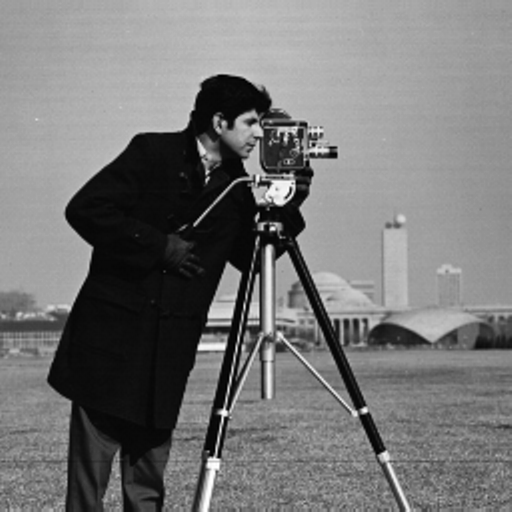
\includegraphics[width=\textwidth]{blurred_image_example_orig}
  \caption{Source image\\$h[n,p]$}
  \label{fig:source_image}
 \end{subfigure}
 \hfill
 \begin{subfigure}[b][0.35\textwidth+2\baselineskip]{0.26\textwidth}
  \centering
  \vfill
  
\includegraphics[width=\textwidth]{blurred_image_example_kernel}%
  \captionsetup{justification=centering}
  \vfill
  \caption{Point-spread function\\$\chi_s[n,p;N/2,L-1]$}
  \label{fig:point_spread_function}
 \end{subfigure}
 \hfill
 \begin{subfigure}[b]{0.35\textwidth}
  \centering
  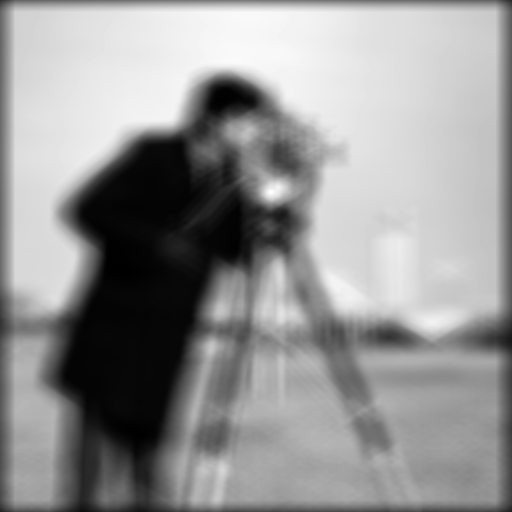
\includegraphics[width=\textwidth]{blurred_image_example_blurred}
  \caption{Blurred image\\$u[n',p']$}
  \label{fig:blurred_image}
 \end{subfigure}
 \caption[Image blurring example]{\emph{Image blurring example.} A blurred image \textbf{(\subref{fig:blurred_image})} is formed by an inner product between a source image \textbf{(\subref{fig:source_image})} and a point-spread function \textbf{(\subref{fig:point_spread_function})}. The point-spread function describes how a block of neighboring pixels in the source image is weighted and combined to get a single pixel value in the blurred image. Because the point-spread function is shift invariant in this case, the inner product amounts to a two-dimensional convolution.}
 \label{fig:image_blurring}
\end{figure}%
Mathematically, this type of blurring takes the form of an inner product between the source image $h[n,p]$ and the point-spread function $\chi_s[n,p;n',p']$:
\begin{equation}\label{eq:image_blurring}
 u[n',p'] = \innerprod[\Big]{h[n,p]}{\chi_s[n,p;n',p']} = \sum_{p=0}^{P-1} \sum_{n=0}^{N-1} h[n,p] \chi_s^*[n,p;n',p'],
\end{equation}
where $\innerprod{\cdot}{\cdot}$ denotes an inner product (two-dimensional over the $n$ and $p$ indices in this case) and $u[n',p']$ is the resulting blurred image.

In terms of the radar analogy, the resulting image $u[n',p']$ is the output of matched filtering performed on the received signal, the point-spread function $\chi_s[n,p;n',p']$ is the ambiguity function, and the source image $h[n,p]$ is the reflectivity of the target scene. The matched filter bank result was originally defined in Section \ref{matched_filtering}; it is calculated from the received signal $y[m]$ according to
\begin{equation}\label{eq:matched_filtering_for_model}
 u[n',p'] = \sum_{m=0}^{M-1} s^*[m - p' + L-1]\, e^{-2\pi i n' (m-p'+L-1)/N}\, y[m],
\end{equation}
where $s[l]$ represents the transmitted waveform and $y[m]$ represents the received signal. The ambiguity function $\chi_s[n,p;n',p']$ for the code $s[l]$ was also defined earlier, in Section \ref{radar_ambiguity}; it describes how matched filtering takes a point in delay-frequency space and spreads it into sidelobes:
\begin{multline}
 \chi_s[n,p;n',p'] = \sum_{m=0}^{M-1} s[m - p' + L - 1]\, e^{2\pi i n' (m-p'+L-1)/N}\\
 \times s^*[m - p + L - 1]\, e^{-2\pi i n (m-p+L-1)/N}.
\end{multline}
The target reflectivity $h[n,p]$ is something we have not yet encountered; it is a matrix of complex numbers that represents the magnitude and phase of the reflected signal (including the power gains and losses described by the radar equation \eqref{eq:radar_equation}) as indexed by delay $p$ and frequency $n$. In this way it is very much like a complex-valued image of delay-frequency space. Substituting these representations into the blurring equation, \eqref{eq:image_blurring}, will allow us to define a mathematical radar model.

\subsection{Ambiguity Equation}
First, though, it is convenient to simplify these equations by assigning an operator name, $A^*$, to matched filtering. By defining $A^*$ as
\begin{equation}
 A^*(y)[n,p] = \frac{1}{\sqrt{N}} \sum_{m=0}^{M-1} s^*[m - p + L-1]\, e^{-2\pi i n (m-p+L-1)/N}\, y[m],
\end{equation}
equation \eqref{eq:matched_filtering_for_model} can be written compactly as
\begin{equation}\label{eq:matched_filtering_with_operator}
 u[n',p'] = \sqrt{N} A^*\paren[\big]{y[m]}.
\end{equation}
As the notation indicates, $A^*$ is a function that takes a one-dimensional vector of length $M$ and produces a two-dimensional matrix with indices $n$ and $p$ of lengths $N$ and $P$. The matched filter operator also has an adjoint or conjugate transpose, $A$, defined by the inner product identity:
\begin{align}
 \innerprod[\Big]{A(x)}{y[m]} &= \innerprod[\Big]{x[n,p]}{A^*(y)}.
 %&= \frac{1}{\sqrt{N}} \sum_{p=0}^{P-1} \sum_{n=0}^{N-1} \brak*{x[n,p] \cdot \paren*{\sum_{m=0}^{M-1} s^*[m - p + L-1]\, e^{-2\pi i n (m-p+L-1)/N}\, y[m]}^*}\\
 %&= \frac{1}{\sqrt{N}} \sum_{m=0}^{M-1} \brak*{\paren*{\sum_{p=0}^{P-1} \sum_{n=0}^{N-1} s[m - p + L-1]\, e^{2\pi i n (m-p+L-1)/N} x[n,p]} \cdot y^*[m]}
\end{align}
From this, we can write $A$ on its own as
\begin{equation}
 A(x)[m] = \frac{1}{\sqrt{N}} \sum_{p=0}^{P-1} \sum_{n=0}^{N-1} s[m - p + L-1]\, e^{2\pi i n (m-p+L-1)/N}\, x[n,p].
\end{equation}
Again following the notation, $A$ is a function that takes a two-dimensional matrix as its argument and produces a one-dimensional vector indexed by $m$. The scaling factor of $1/\sqrt{N}$ is included in the definitions for both $A^*$ and $A$ because it ensures that the compound operator $AA^*(y)$ is the identity scaled by $\norm{2}{s}^2$. Accordingly, it is convenient to define scaled reflectivity coefficients $x[n,p]$ as
\begin{equation}
 x[n,p] = \sqrt{N} h[n,p] \quad \Leftrightarrow \quad h[n,p] = \frac{1}{\sqrt{N}} x[n,p].
\end{equation}

The measurement ambiguity equation can be formed by substituting the radar representations for the image blurring terms back into equation \eqref{eq:image_blurring}:
\begin{align}
 \sqrt{N} A^*\paren[\big]{y[m]}
 &= \begin{multlined}[t]
     \sum_{p=0}^{P-1} \sum_{n=0}^{N-1} \frac{1}{\sqrt{N}} x[n,p] \sum_{m=0}^{M-1} s^*[m - p' + L - 1]\, e^{-2\pi i n' (m-p'+L-1)/N}\\
     \times s[m - p + L - 1]\, e^{2\pi i n (m-p+L-1)/N}
    \end{multlined}\nonumber\\
 &= \begin{multlined}[t]
     \sum_{m=0}^{M-1} s^*[m - p' + L - 1]\, e^{-2\pi i n' (m-p'+L-1)/N}\\
     \times \frac{1}{\sqrt{N}} \sum_{p=0}^{P-1} \sum_{n=0}^{N-1} s[m - p + L - 1]\, e^{2\pi i n (m-p+L-1)/N}\, x[n,p].
    \end{multlined}\\
\intertext{Further simplification is possible by writing the right-hand side in terms of the $A$ and $A^*$ operators:}
 A^*\paren[\big]{y[m]}
 &= \frac{1}{\sqrt{N}} \sum_{m=0}^{M-1} s^*[m - p' + L - 1]\, e^{-2\pi i n' (m-p'+L-1)/N} A\paren[\big]{x[n,p]}\nonumber\\
 &= A^*\paren*{A\paren[\big]{x[n,p]}}.
\end{align}
We call this the ambiguity equation since it relates the ambiguous matched filter output to the artifact-free reflectivity coefficients, and the composed operator $A^*A$ completely describes the resulting delay-frequency sidelobes. Since it is easy to overlook, note that we now have the following definitions in terms of the operators $A$ and $A^*$:
\begin{align}
 \text{Matched filter bank applied to $y$:} \quad & \sqrt{N} \cdot A^*\paren{y}\label{eq:mf_Astar}\\
 \text{Ambiguity function centered at ($n_0 , p_0$):} \quad & N \cdot A^*A\paren*{\delta_{n_0,p_0}}\label{eq:ambiguity_AstarA},
\end{align}
where $\delta_{n_0,p_0}[n,p]$ is the discrete delta function that returns 1 at [$n_0 , p_0$] and 0 otherwise.

\subsection{The Radar Model}
The ambiguity equation is close to what we desire for a radar model, but one further simplification can be made. Since both sides of the equation have matched filtering applied to them, $A^*$ can be removed to arrive at a measurement equation:
\begin{equation}\label{eq:radar_model_with_operator}
 y[m] = A\paren[\big]{x[n,p]}.
\end{equation}
The measured radar signal $y[m]$ is now just a linear function of the scaled delay-frequency target reflectivity $x[n,p]$. That linear function, $A$, is the radar model. Interestingly, the radar model is the adjoint, or conjugate transpose, of the matched filter bank operation. This means that while the matched filter correlates the received signal with the expected return from point targets with different delays and frequency shifts, the radar model simulates the received signal as the sum of returns from point targets with different delays and frequency shifts. Though that mirror relationship is just something of a curiosity for now, it will have importance later when it comes to solving for the target reflectivity.

The radar model equation is useful because it provides the formalism needed for eliminating delay-frequency sidelobes: one can use the measured signal and radar model to solve for the target reflectivity. As formulated, the target reflectivity is precisely the matched filter result but with sidelobes removed. Unfortunately, it is not a straightforward process to just solve for the target reflectivity. The radar model is not invertible because equation \eqref{eq:radar_model_with_operator} is under-determined, with more unknowns in the target reflectivity than equations provided by the measurements; this is a natural consequence of allowing for unknown frequency shifts. Since the system of equations is under-determined, there are an infinite number of solutions for the target reflectivity function that would satisfy the equation and match the measurements. The matched filter result is one of those solutions, but it has serious shortcomings. Finding the best solution for the target reflectivity is the subject of Part \ref{part_waveform_inversion}, where it will be shown that sparsity of the radar scene is key to eliminating sidelobes.

Fully written out, the radar model is:
\begin{align}
 y[m] &= \frac{1}{\sqrt{N}} \sum_{p=0}^{P-1} \sum_{n=0}^{N-1} s[m - p + L-1]\, e^{2\pi i n (m-p+L-1)/N}\, x[n,p] \label{eq:radar_model_x}\\
 \intertext{or equivalently}
 y[m] &= \sum_{p=0}^{P-1} \sum_{n=0}^{N-1} s[m - p + L-1]\, e^{2\pi i n (m-p+L-1)/N}\, h[n,p]. \label{eq:radar_model}
\end{align}
In the theory of vector spaces, the model $A$ is a tight frame, conceptually the equivalent of an overcomplete basis for delay-frequency space. In fact, the model is an instance of a Gabor frame with window given by the code $s$, also known as a short time Fourier transform \autocite{Mal08}. This representation can be interpreted using the notion of a grid of point targets, which is visualized in Figure \ref{fig:delay_frequency_grid}.
\begin{figure}[tpb]
 \centering
 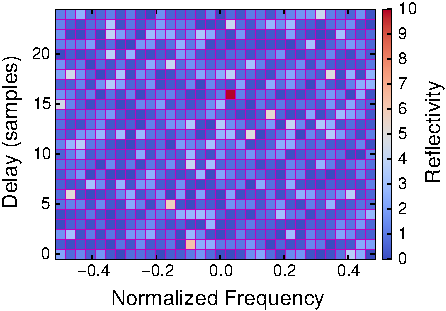
\includegraphics{range_doppler_discretization}
 \caption[Reflectivity coefficients as a delay-frequency grid of point targets]{\emph{Reflectivity coefficients as a delay-frequency grid of point targets.} Each grid point represents a location in delay-frequency space indexed by delay $p$ and frequency $n$. The color of each point corresponds to the amount of signal reflected at that particular delay and frequency shift, a value given by the magnitude of the target reflectivity coefficient $h[n,p]$. The radar scene is thus represented by a grid of independent point targets according to the radar model of equation \eqref{eq:radar_model}.}
 \label{fig:delay_frequency_grid}
\end{figure}%
The target reflectivity $h[n,p]$ can be thought to represent point targets distributed uniformly over delay-frequency space. Each point target can reflect the transmitted radar waveform independently with a given magnitude and phase. The radar model describes how reflections from each of these point targets would manifest in the measured signal, and it sums the contributions of each to produce the measurement. Again, this is just the mirror operation to what the matched filter does in its role as adjoint, assuming point targets in delay-frequency space and matching against the modeled reflection.

\section{Derivation of Radar Model}
\label{radar_model_derivation}
\subsection{Narrow-band Received Signal}
Though we now have a suitable radar model, it is instructive to derive it in another way that will allow us to relate the discrete reflectivity coefficients $h[n,p]$ to the complete reflectivity function. We begin with the narrow-band radar equation for (the complex envelope of) the baseband received signal from a fluctuating distributed target \autocite{VTre01}:
\begin{equation}
 y(t) = \int_{\rho_0}^{\rho_1} s(t - \rho) \tilde{a}\paren*{t - \frac{\rho}{2}, \rho} \dee\rho,
\end{equation}
where $s(t)$ is the transmitted baseband modulation signal and $\tilde{a}(t, \rho)$ is the complex target reflectivity (magnitude and phase) as a function of time $t$ and delay $\rho$. Note that this reflectivity function encompasses the power gained and lost according to the radar equation \eqref{eq:radar_equation}; it is not just the fraction of reflected power as described by the radar cross section $\sigma$. We have taken the integration interval to be $\brak*{\rho_0, \rho_1}$ to reflect the limited sampling window, and this carries with it the implicit assumption that $\tilde{a}(t - \rho/2, \rho) = 0$ outside that range. Whether one considers $\tilde{a}(t, \rho)$ to be random or deterministic does not matter at present. To ease further derivation, we define a new function
\begin{equation}
 \tilde{h}(t, \rho) = \tilde{a}\paren*{t + \frac{\rho}{2}, \rho}
\end{equation}
so that the time variable represents the scattering for a signal \emph{sent} at time $t$ (which arrives at the target at $t + \rho/2$) rather than one reaching the target at time $t$. This results in
\begin{equation}\label{eq:continuous_measurement}
 y(t) = \int_{\rho_0}^{\rho_1} s(t - \rho) \tilde{h}(t - \rho, \rho) \dee\rho.
\end{equation}

\subsection{Discretization}
The next step is to begin discretizing the model. We assume that the received signal is sampled at a uniform rate $\tau_s$ starting at time $t_0$ and ending at $t_1$ (inclusive), so that $y(t)$ is represented by a complex discrete sequence
\begin{align}
 y[m] = y(m\tau_s + t_0) && m = 0,\dotsc,M-1 && M = (t_1 - t_0)/\tau_s + 1.
\end{align}
In addition, we restrict our attention to discrete phase-modulated signals with $L$ bauds and a baud length of $\tau_b$, so that
\begin{equation}
 s(t) = s[l]\quad \text{for}\quad l\tau_b \le t < (l + 1)\tau_b, \quad l = 0,\dotsc,L-1
\end{equation}
for a complex sequence $s[l] \in \field{C}$. For ease of notation, let us also infinitely extend the sequence $s[l]$ by letting its value for non-existent indices be zero, $s[l] = 0$ for $l \ne 0,\dotsc,L-1$. If we assume that the sampling time is an integer multiple of the baud length, then we have $\tau_s = R\tau_b$ where $R$ is the under-sampling ratio. Note that if the reverse is true and over-sampling by an integer ratio is performed, we can simply duplicate the modulation sequence by the over-sampling ratio and let $R=1$. Finally, the time interval $[t_0, t_1]$ can be chosen to correspond to the delay interval $[\rho_0, \rho_1]$ by requiring $t_0 = \rho_0 + L\tau_b$ and $t_1 = \rho_1$. This shrinks the sampling window to ensure that all returns from outside of the delay window have no contribution to the samples (each delay affects multiple later measurements because of the length of the code). Because of this relationship, we know that the delay integration window can be divided into $(\rho_1 - \rho_0)/\tau_b = R(M-1) + L \equiv P$ equal segments of size $\tau_b$. With these assumptions, we can break up the integral in equation \eqref{eq:continuous_measurement} as follows:
\begin{align}\label{eq:discrete_transmission}
 y[m] &= y(m\tau_s + t_0)\nonumber\\
 &= \int_{\rho_0}^{\rho_1} s(m\tau_s + t_0 - \rho) \tilde{h}(m\tau_s + t_0 - \rho, \rho) \dee\rho\nonumber\\
 &= \sum_{p=0}^{RM+L-R-1} \int\limits_{\rho_0 + p\tau_b}^{\rho_0 + (p+1)\tau_b} s(Rm\tau_b + L\tau_b + \rho_0 - \rho) \tilde{h}(Rm\tau_b + L\tau_b + \rho_0 - \rho, \rho) \dee\rho\nonumber\\
 &= \sum_{p=0}^{P-1} s[Rm-p+L-1] \int\limits_{p\tau_b}^{(p+1)\tau_b} \tilde{h}(Rm\tau_b + L\tau_b - \rho, \rho + \rho_0) \dee\rho.
\end{align}

\subsection{Simplification}
Now comes a key observation: $s(t)$ is nonzero only over $0 \leq t < L\tau_b$, and $\tilde{h}(t, \rho)$ is evaluated over the same values in equation \eqref{eq:continuous_measurement}. Thus, the result of the model will be the same if we replace $\tilde{h}(t, \rho)$ with its Fourier series representation on the interval $0 \leq t \leq N\tau_b$, where $N \geq L$ and $\nu_0 = 1/(N\tau_b)$ is the smallest frequency component. The Fourier series is given by
\begin{equation}
 \tilde{h}(t, \rho) = \sum_{k = -\infty}^{\infty} h_k(\rho) e^{2\pi i k \nu_0 t} \quad \text{for} \quad 0 \leq t \leq 1/\nu_0,
\end{equation}
where
\begin{equation}\label{eq:fourier_series_coefficients}
 h_k(\rho) = \nu_0 \int_{0}^{1/\nu_0} \tilde{h}(t, \rho) e^{-2\pi i k\nu_0 t} \dee t
\end{equation}
defines the Fourier coefficients. Substituting the Fourier series representation into equation \eqref{eq:discrete_transmission} yields
\begin{multline}
 y[m] = \sum_{p=0}^{P-1} s[Rm-p+L-1]\\
 \times \int\limits_{p\tau_b}^{(p+1)\tau_b} \sum_{k = -\infty}^{\infty} h_k(\rho + \rho_0) e^{2\pi i k(Rm + L)/N} e^{-2\pi i k\nu_0 \rho} \dee\rho.
\end{multline}
This seems to have made the model more complicated for no benefit: there are now three discrete parameters and an infinite sum to boot. Notice, however, that $e^{2 \pi i k(Rm+L)/N}$ as a function of $k$ is periodic with period $N$. Re-parameterizing the infinite sum leads to
\begin{multline}
 y[m] = \sum_{p=0}^{P-1} s[Rm-p+L-1] \\
 \times \sum_{n=0}^{N-1} e^{2 \pi i n(Rm+L)/N} \int\limits_{p\tau_b}^{(p+1)\tau_b} \sum_{k = -\infty}^{\infty} h_{n + kN}(\rho + \rho_0) e^{-2\pi i (n + kN) \nu_0 \rho} \dee\rho.
\end{multline}
Now the result of the integral is indexed by $n$ and $p$ where $n$ parameterizes the frequency domain and $p$ parameterizes the delay domain. However, it doesn't quite match the earlier radar model definition in equation \eqref{eq:radar_model}. Factoring out the required terms produces
\begin{multline}
 y[m] = \sum_{p=0}^{P-1} \sum_{n=0}^{N-1} s[Rm-p+L-1] e^{2 \pi i n(Rm-p+L-1)/N}\\
 \times e^{2 \pi i n(p+1)/N} \int\limits_{p\tau_b}^{(p+1)\tau_b} \sum_{k = -\infty}^{\infty} h_{n + kN}(\rho + \rho_0) e^{-2\pi i (n + kN) \nu_0 \rho} \dee\rho.
\end{multline}
The form of this equation matches, and thus we define the discrete reflectivity coefficients as
\begin{equation}\label{eq:reflectivity_coefficients_not_simplified}
 h[n,p] = e^{2 \pi i n(p+1)/N} \int\limits_{p\tau_b}^{(p+1)\tau_b} \sum_{k = -\infty}^{\infty} h_{n + kN}(\rho + \rho_0) e^{-2\pi i (n + kN) \nu_0 \rho} \dee\rho
\end{equation}
and arrive once again at the discrete linear radar model:
\begin{equation}\label{eq:radar_model_with_R}
 y[m] = \sum_{p=0}^{P-1} \sum_{n=0}^{N-1} s[Rm-p+L-1] e^{2 \pi i n(Rm-p+L-1)/N} h[n,p].
\end{equation}
The only difference this time is the generalization to include undersampling of the transmitted waveform by a factor of $R$.

\subsection{Assumptions}
To sum up the derivation, recall the assumptions that underpin this model. We started with the narrow-band radar equation, which assumes that the bandwidth of the signal is much smaller than the baseband frequency so that the Doppler effect can be approximated only by frequency shifts and not time dilation. We also made the standard assumption that there is no scattering from outside the ranges parametrized by the model. In terms of the discretization, we assumed that the received signal is uniformly sampled at a fixed rate and that the transmitted waveform is piecewise constant over uniform intervals. We also required a uniformly-spaced frequency index with a number of frequency steps $N$ greater than the number of bauds $L$ in the transmitted waveform. All of these assumptions are congruous with standard radar practices and none are overly restrictive. From this we get an exact representation of the complete target reflectivity function as a discrete set of reflectivity coefficients $h[n,p]$.

\section{Representation of Targets}
\label{radar_model_representation}
\subsection{Deterministic Reflectivity}
The radar model allows us to analyze measurements in terms of delay-frequency reflectivity coefficients $h[n,p]$, but it is unclear as of yet how these coefficients embody actual radar target scenes. It is easy to think of the coefficients as representing a grid of point targets with different delays and frequency shifts, but this is highly unlikely to be the physical reality. Fortunately, the radar model derivation provides an exact relationship between the reflectivity coefficients and the complete reflectivity function, equation \eqref{eq:reflectivity_coefficients_not_simplified}, that we can use to provide an intuitive interpretation. As shown in Appendix \ref{reflectivity_coefficients}, the reflectivity coefficient equation can be simplified to
\begin{align}\label{eq:reflectivity_coefficients}
 h[n,p] = \int\limits_{p\tau_b}^{(p+1)\tau_b} \brak*{h(f, \rho + \rho_0) e^{-2\pi i f (\rho - (p+1)\tau_b)} * b_{N,\tau_b}(f)}\!(n\nu_0) \dee\rho,
\end{align}
where the new term $b_{N,\tau_b}(f)$ is a frequency-blurring kernel involving the periodic sinc function. This kernel is defined as
\begin{align}
 b_{N,\tau_b}(f) &= e^{-\pi i \tau_b f (N-1)} \mathrm{psinc}_N(2\pi \tau_b f)\\
 &= \frac{1}{N} e^{-\pi i \tau_b f (N-1)} \frac{\sin(\pi N \tau_b f)}{\sin(\pi \tau_b f)},
\end{align}
and the periodic sinc function $\mathrm{psinc}_N(2\pi \tau_b f)$ is plotted in Figure \ref{fig:periodic_sinc} for reference.
\begin{figure}[tpb]
 \centering
 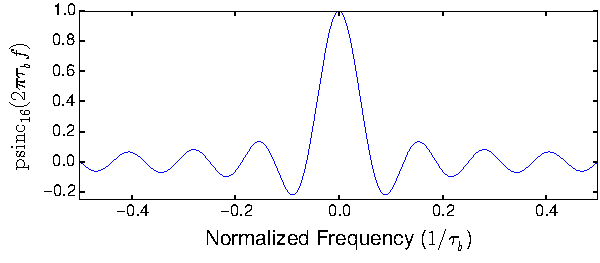
\includegraphics{periodic_sinc}
 \caption[Periodic sinc]{\emph{Periodic sinc.} The periodic sinc function, shown here for $N=16$, results from taking the discrete-time Fourier transform of the $N$-sample wide rect function. It is periodic over the width of the displayed frequency window, $1/\tau_b$.}
 \label{fig:periodic_sinc}
\end{figure}%
If the reflectivity function $h(f, \rho)$ is taken to be deterministic, the interpretation of equation \eqref{eq:reflectivity_coefficients} is straightforward: in the Doppler frequency variable $n$, the coefficients represent samples from the reflectivity function frequency spectrum $h(f, \rho)$ after it has been "smeared" by $b_{N,\tau_b}(f)$ through convolution; in the time delay variable $p$, the coefficients represent an integration of the reflectivity function over the corresponding delay window.

\subsection{Probabilistic Reflectivity}
Concerning the more general case of a probabilistic reflectivity function, we invoke the doubly-spread target model of \textcite{VTre01}: assume that the reflectivity function $h(f, \rho)$ is a zero-mean complex Gaussian random variable with autocovariance given by
\begin{equation}
 \mathrm{E}\brak*{h(f, \rho) h^{*}(f', \rho')} = S(f, \rho) \delta(f - f') \delta(\rho - \rho'),
\end{equation}
where $\mathrm{E}[\cdot]$ denotes expected value and $S(f, \rho)$ is the scattering function describing the returned \emph{power} as a function of frequency and range. The process is zero-mean because the phase of $h(f, \rho)$ is assumed to follow a uniform distribution that is independent of the magnitude. In practical terms, the main difference between the deterministic model and the doubly-spread model is the phase of the returned signal: the former model produces phases that are a fixed function of range, while the latter model produces random phases with respect to range. Which of these is appropriate will depend upon the application; the deterministic model is best for simple targets with a known form, while the probabilistic model is best for targets that vary over time or present upredictably complex scattering. Fortunately, both formulations fit equally well with the radar model. In terms of the reflectivity coefficients, the doubly-spread target model results in
\begin{equation}\label{eq:reflectivity_coefficients_doubly_spread}
 \mathrm{E}\brak*{h[n,p]h^*[n,p]} = \int\limits_{p\tau_b}^{(p+1)\tau_b} \brak*{S(f, \rho + \rho_0) * B(f)}\!(n\nu_0) \dee\rho
\end{equation}
with
\begin{align}
 B(f) &= \mathrm{psinc}_N^2(2\pi \tau_b f)\\
 &= \frac{1}{N^2} \frac{\sin^2(\pi N\tau_b f)}{\sin^2(\pi \tau_b f)}.
\end{align}
In this case, the relationship between the coefficients and the actual quantity of interest $S(f, \rho)$ is even clearer: on average, the coefficients $\abs[\big]{h[n,p]}^2$ give the total power returned by the target from ranges $p\tau_b \le \rho - \rho_0 < (p+1)\tau_b$ and frequencies weighted by the squared periodic sinc $B(n\nu_0 - f)$. Both the deterministic and doubly-spread target models lead to similar interpretations for the reflectivity coefficients; the difference is in how the phases of the returned signals add up.

\subsection{Reflectivity Coefficient Sparsity}
\label{point_target_reflectivity}
With the deterministic and probabilistic interpretations of the reflectivity coefficients in hand, we can finally address a matter of vital importance: under what conditions are the reflectivity coefficients sparse? Recall that radar scenes are typically sparse, with scatterers occupying only a small portion of delay-frequency space. Thus, the complete reflectivity function $h(f, \rho)$ can be assumed to have sparse support. The hope is that this sparsity translates into sparsity of the reflectivity coefficients. If it does, we can use that prior knowledge to find the sparsest solution for $h[n,p]$ that matches the measurements according to the radar model and have confidence that it is the true sidelobe-free solution.

To illustrate the reflectivity coefficient interpretations and analyze the coefficient sparsity for the sparsest possible target, consider the case of a point target with a reflectivity of $A$ initially at range $r$ and traveling toward the radar with a range rate $v$. The target's time delay and Doppler frequency shift are given by $\rho_t \approx \frac{2r}{c}$ and $f_t \approx \frac{2v}{c}f_0$ respectively, where $c$ denotes the speed of light and $f_0$ is the baseband radar frequency. The appropriate target reflectivity function is
\begin{align}
 \tilde{h}(t, \rho) &= A e^{2\pi i f_t t} \delta(\rho - \rho_t) e^{2\pi i f_t \rho} e^{-2\pi i f_0 \rho_t}\\
\intertext{or equivalently}
 h(f, \rho) &= A \delta(f - f_t) \delta(\rho - \rho_t) e^{2\pi i f_t \rho} e^{-2\pi i f_0 \rho_t}.
\end{align}
Plugging this into equation \eqref{eq:reflectivity_coefficients} shows how the discrete model represents a point target:
\begin{equation}
 h[n,p] = \begin{cases}
            A\, b_{N,\tau_b}(n\nu_0 - f_t) e^{2\pi i f_t(\rho_0 + (p+1)\tau_b)} e^{-2\pi i f_0 \rho_t} & p = p_t\\
            0 & p \neq p_t,
           \end{cases}
\end{equation}
where $p_t$ gives the delay index which satisfies $p_t\tau_b \leq \rho_t - \rho_0 < (p_t+1)\tau_b$. In order to look at sparsity, it will be easier to visualize the magnitude of the reflectivity coefficients. This is given by
\begin{equation}\label{eq:point_target_coefficients}
 \abs[\Big]{h\brak[\big]{n,p_t}} = \frac{A}{N} \abs*{\frac{\sin\paren[\big]{\pi N\tau_b (n\nu_0 - f_t)}}{\sin\paren[\big]{\pi\tau_b (n\nu_0 - f_t)}}}.
\end{equation}
Example point target reflectivity coefficients given by equation \eqref{eq:point_target_coefficients} are shown in Figure \ref{fig:point_target_coefficients}.
\begin{figure}[tpb]
 \centering
 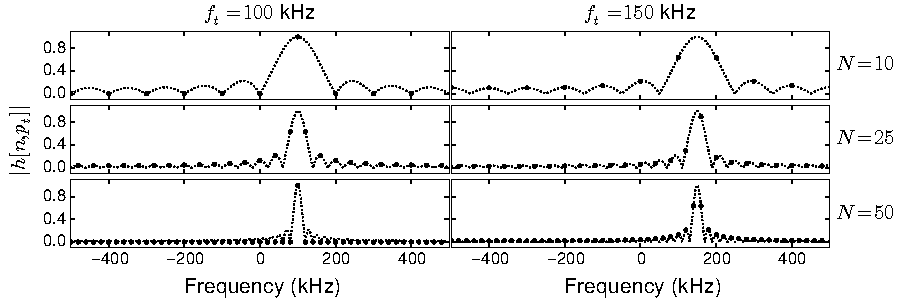
\includegraphics{point_target_coefficients}
 \caption[Reflectivity coefficients for point targets]{\emph{Reflectivity coefficients for point targets.} The reflectivity coefficient magnitudes are given by equation \eqref{eq:point_target_coefficients} with $A = 1$ and $\tau_b = 1 \, \mu\textrm{s}$ as a function of frequency for six point target cases. The left column shows the values for a point target with Doppler frequency shift of 100 kHz, while the right column shows values for a Doppler shift of 150 kHz. The first row shows the coefficient values when 10 frequencies are included in the discrete model, the second row shows values for 25 frequencies, and the third row shows values for 50 frequencies. The dotted line in each plot shows the underlying curve from which the coefficients are sampled.}
 \label{fig:point_target_coefficients}
\end{figure}%
Notice that if $n_t\nu_0 = f_t$ for some integer $n_t$, then all of the coefficients are zero except for $h[n_t,p_t]$ and target sparsity translates directly into coefficient sparsity. However, in general all of the frequency coefficients corresponding to the correct range will be nonzero, and the question then becomes one of degree: are there few enough significant coefficients to say that they are sparse? In practical terms, "significant" means being above the noise level, since smaller values can be taken as zero and the reconstruction error will still be acceptable.

Figure \ref{fig:point_target_coefficients} suggests one way of ensuring that the coefficient sparsity emulates the reflectivity function sparsity for point targets and by extension any general target: increasing $N$, the number of frequencies included in the discrete model. As $N$ increases, the discretization effects become more localized and the values $h[n,p_t]$ for the point target look more like direct frequency samples from $h(f, \rho_t)$. This is a consequence of the frequency-smearing interpretation of the relationship between the reflectivity function and coefficients. Since the periodic sinc becomes more delta-like as $N$ increases, the smearing it produces decreases. It is important to note that this is the same problem and solution encountered when relating the discrete Fourier transform of a sampled function to the complete function's Fourier transform. So we conclude that in general with $N$ large enough, sparsity of $h(f, \rho)$ for any target translates directly to sparsity of $h[n,p]$.
\part{Waveform Inversion}
\label{part_waveform_inversion}
\graphicspath{{chapters/sparsity_background/figures/}}
\chapter{Sparse Solutions of Underdetermined Systems}
\label{sparsity_background}
The method of least squares has been used for fitting models to data since Gauss invented the normal distribution and used it to predict the orbits of celestial bodies \autocite{Sti81}. With the law of large numbers ensuring that measurements often have Gaussian error, least squares serves its role well when no other prior information can be employed. This chapter is about the case when that isn't true, when we know something about the form of the solution itself: it is sparse. Images and audio are sparse; radar scenes are sparse; the brain uses sparsity to make sense of the world. Whenever something looks complex but is actually simple in the right form, that's sparsity. Across many applications, sparsity serves as a useful representation of prior knowledge.

The use of sparsity for inversion or fitting falls under a number of umbrella terms: compressed sensing, sparse approximation, low-rank decomposition, $l_1$-regularization, and many similar variants. Each of these means something slightly different, but the machinery behind them is the same. In all cases, a simple or sparse representation is sought for some data, and the key to getting it is a nonlinear method. The solution methods are more diverse than even the number of applications for them, and the list continues to grow. For our purposes, we will focus on the theory of compressed sensing because it provides good guidance for what kind of approaches will work best. We will also focus on solution methods based on convex optimization and particularly the prox operator, since these are easy to understand, flexible, have good theoretical underpinnings, and perform well in practice \autocite{PB13}. However, this choice is still somewhat arbitrary; the approach is the important part, and not so much the particular methods used.

\section{Underdetermined Systems of Equation}
\label{underdetermined_systems}
When performing model inversion, a common challenge is solving an underdetermined system of equations. In this situation, one has a matrix/vector equation such as
\begin{equation}
 y = Ax,
\end{equation}
where $y$ is a vector of length $M$ representing measurements, $A$ is a matrix that encompasses the mathematical model of the system, and $x$ is a vector of length $N$ giving unknown parameters. The equation is underdetermined because there are fewer measurements in $y$ than unknowns in $x$, so there are an infinite number of $x$ vectors that satisfy the equation. This situation can arise in many ways, but in general we can think of the underdetermined system as representing the decomposition of a signal $y$ using an overcomplete dictionary. The columns of the matrix $A$, denoted $a_n$, are the atoms of the dictionary, and the entries of $x$ are the coefficients corresponding to those atoms:
\begin{equation}
 y = \sum_{n=0}^{N-1} x[n] a_n.
\end{equation}
Since $M < N$, the dictionary atoms cannot form an orthogonal set, and there are many ways to form the decomposition \autocite{Mal08}. "Solving" the underdetermined system involves finding a preferable decomposition, one that at least has the qualities of the original measurement-generating solution when they are not the same.

\subsection{Least Norm Solution}
A common and linear solution method to an underdetermined system of equations is to take a least norm approach. Of the infinite number of solutions, it is simple to find the one with the smallest $l_2$-norm by performing the optimization
\begin{equation*}\tag{$\text{P}_\text{2}$}
 \begin{matrix*}[l]
  \underset{x}{\mathrm{minimize}} & \norm{2}{x}\\
  \text{subject to} & y = Ax,
 \end{matrix*}
\end{equation*}
where $\norm{2}{x} = \sum_k \abs{x[k]}^2$ denotes the $l_2$-norm. When $A$ is full rank (none of the measurements are redundant), $AA^*$ is invertible and the solution to the least norm problem is
\begin{equation}\label{eq:least_norm_solution}
 x_* = A^*(AA^*)^{-1}y.
\end{equation}
For situations when the measurements are noisy, one can turn to the related $l_2$-regularized least squares problem, also known as Tikhonov regularization:
\begin{equation*}\tag{$\text{P}_{\text{2}\lambda}$}
 \underset{x}{\mathrm{minimize}} \quad \norm{2}{y - Ax} + \lambda\norm{2}{x},
\end{equation*}
where $\lambda$ is the regularization parameter. This problem is solved by calculating 
\begin{equation}
 x_* = (A^*A + \lambda I)^{-1} A^* y,
\end{equation}
where $I$ is the identity matrix. As $\lambda \rightarrow 0$, the solution to $l_2$-regularized least squares converges to the least norm solution. Since these solutions are the result of basic matrix operations and are therefore linear, they are often favored for their ease of computation \autocite[Lecture 8]{Boy08}.

\subsection{Sparsest Solution}
Motivated by the inherent simplicity of answers to many practical problems, another approach to selecting a particular solution of an underdetermined system is to choose the sparsest solution. This problem can be written using the $l_0$ pseudo-norm, which is just the count of the number of nonzero entries in a vector:
\begin{equation}
 \norm{0}{x} = \#\set{k : x[k] \ne 0}.
\end{equation}
With this notation, the sparsest solution is found by the optimization problem
\begin{equation*}\tag{$\text{P}_\text{0}$}
 \begin{matrix*}[l]
  \underset{x}{\mathrm{minimize}} & \norm{0}{x}\\
  \text{subject to} & y = Ax.
 \end{matrix*}
\end{equation*}
Unfortunately, this problem is NP-hard in general \autocite{Nat95}, requiring combinatorial optimization to solve. Essentially, one has to check each sparsity pattern (location of zeros/nonzeros) for a solution until the sparsest one is found.

Fortunately, the convex relaxation of this problem, which is easy to solve, provides the sparsest solution in most cases. Instead of minimizing the $l_0$ pseudo-norm, one minimizes the $l_1$-norm:
\begin{equation*}\tag{$\text{P}_\text{1}$}\label{eq:l1min}
 \begin{matrix*}[l]
  \underset{x}{\mathrm{minimize}} & \norm{1}{x}\\
  \text{subject to} & y = Ax,
 \end{matrix*}
\end{equation*}
where $\norm{1}{x} = \sum_k \abs{x[k]}$ denotes the $l_1$-norm. Then for the overwhelming majority of matrices $A$ with columns normalized to one, there is a constant $\rho(M, N) > 0$ such that if $x_0$ is a solution to $y=Ax_0$ with at most $\rho M$ nonzeros, that solution is both the sparsest possible solution and the minimal $l_1$-norm solution \autocite{Don06}. In other words, whenever there is a sufficiently sparse solution, $l_1$ minimization will find it. The proof by \textcite{Don06} does not provide a practically useful formula for the breakdown point $\rho$, but it does provide motivation for why an equivalence of this kind must exist. It is easy to see how the $l_1$-norm promotes sparse solutions by equally penalizing both large and small nonzero values of $x$; equivalence comes from the rarity of truly sparse $x$ that actually solve the underdetermined system, causing $l_1$-minimization to pick out the true solution due to lack of other possibilities.

\section{Compressed Sensing}
\label{compressed_sensing}
Compressed sensing \autocite{Don06a, CW08} expands on the theory for solving underdetermined systems of equations when the solution is known to be sparse. It provides guarantees for recovering the true solution to within noise bounds provided that the measurements are "incoherent" and that their number is on the order of the solution sparsity. In essence, one only needs to measure at the information rate (sparsity) of the solution rather than fully sample the entire space of solutions. Not only that, but these optimal non-adaptive measurements, pre-determined and embodied in a measurement matrix, are known to perform nearly as well as the best adaptive measurements \autocite{Don06a}. The key is sparsity, which acts as the prior information that enables narrowing in on the one true answer out of the infinite potential answers.

\subsection{Conditions}
The main requirement for invoking the theory of compressed sensing is that the sought signal is sparse, or at least well-approximated by a sparse representation. In terms of a specified dictionary, sparsity requires that the signal be well-represented by a relatively small number of coefficients corresponding to the dictionary atoms. A signal might not be sparse in its natural representation, but that does not mean that it is not sparse in some other representation. Images are generally not sparse when specified by individual pixel values, but they are almost always sparse in a Fourier or wavelet dictionary. The only instance where this is not true is for images with high entropy; they are random and have no structure \autocite{Mal08}. Even if a signal $x$ is not exactly sparse, we say it has an $S$-sparse approximation if $\norm{2}{x - x_S}$ is small, where $x_S$ is the vector of coefficients $x[n]$ with all but the largest $S$ entries set to zero. As the success of lossy compression schemes demonstrate, many signals of interest satisfy at least this compressibility condition.

Measurement incoherence is the second condition for applying the theory of compressed sensing \autocite{CW08}. Consider the simplest case of a 1-sparse signal $x_1$ measured as $y=Ax_1$, with the number of measurements $M$ much less than the dimension of the signal $N$. At least one of the measurements must include a contribution from the nonzero entry of $x_1$ or else recovery from $y$ is impossible. Since we don't know \emph{a priori} which element is the nonzero one and because $M \ll N$, the only way to achieve a high probability of recovery is to have measurements that individually span a large portion of the unknown signal space. Each measurement must be global in some sense, embodying most of the unknown coefficients. This concept is known as measurement incoherence: none of the measurements are very concentrated (coherent) in the unknown space.

In the mathematical theory, incoherence can be guaranteed by a number of different but related conditions. Often it is theoretically convenient to allow the measurements to be random. For an orthogonal set of possible measurements given by the matrix $U$ with scaling $U^*U = N \cdot I$, we can let the measurement matrix $A$ be a random subset of $M$ rows of $U$. The coherence $\mu(U)$ of the measurement set is then defined as
\begin{equation}
 \mu(U) = \max_{k,n} \; \abs[\big]{U[k,n]}^2,
\end{equation}
and it varies in value from a minimum of $1$ to a maximum of $N$ \autocite{CR07}. Thus, the measurements are incoherent under this framework when the set from which they are drawn has $\mu(U)$ close to $1$. The coherence parameter can also be defined for a wider class of probabilistic measurement ensembles, including Gaussian and binary random measurements, as shown by \textcite{CP11}.

Deterministic measurements can have their incoherence measured by the restricted isometry property (RIP) introduced by \textcite{CT06} and expanded upon in \textcite{CRT06}. Let $A_T$ with $T \subset \set{0, \dotsc, N-1}$ denote a subset of the columns of the measurement matrix $A$. Then the $S$-restricted isometry constant $\delta_S$ of $A$ is defined as the smallest number such that
\begin{equation}
 (1 - \delta_S)\norm{2}{x_S}^2 \le \norm{2}{A_T x_S}^2 \le (1 + \delta_S)\norm{2}{x_S}^2
\end{equation}
for all $S$-sparse vectors $x_S$ and all subsets $T$ with $\abs{T} \le S$. The restricted isometry property is satisfied and sufficient incoherence assured for a solution with sparsity $S$ when $\delta_{2S}$ is small enough. This condition ensures that the measurements preserve the distance between any two $S$-sparse solutions, guaranteeing that any $S$-sparse answer is unique.

\subsection{Theoretical Bounds}
If the signal is compressible and incoherent sampling is performed, then essentially we know that each measurement contains a contribution from each of the $S$ coefficients. Intuitively, we might then expect to be able to reconstruct the signal from about $S$ measurements. This idea is made concrete with the incoherent sampling theorem presented below for reconstruction via the $l_1$-minimization problem \eqref{eq:l1min}. No matter the specific setting, the principle of this theorem remains the same: if the sampling is incoherent and we solve an appropriate convex optimization problem, we can reconstruct a signal to within noise and $S$-sparse approximation errors by using on the order of $S\log{N}$ measurements.

In the case where we know the coherence $\mu(U)$ of the measurements, the incoherent sampling theorem requires a number of measurements $M$ that meets the condition $M \ge C \cdot \mu(U) \cdot S \cdot \log{N}$ for a sparsity level $S$ and constant $C$. In the case where measurement incoherence is guaranteed in terms of the restricted isometry property, we require $\delta_{2S} < \sqrt{2} - 1$ for a specified sparsity level $S$. For random Gaussian or binary matrices, the RIP requirement on $\delta_{2S}$ is satisfied with overwhelming probability when $M \ge C \cdot S \cdot \log{(N/S)}$. In either case, the recovery bound has the same form. Denoting the result of the $l_1$-minimization problem as $x_*$, the true solution as $x$, and the best $S$-sparse approximation of $x$ as $x_S$, we have
\begin{equation}
 \norm{2}{x_* - x} \le C_0 \norm{2}{x - x_S},
\end{equation}
where $C_0$ is a small known constant. The coherence parameter result is due to \textcite{CP11}, while the RIP result is due to \textcite{Can08}. Both articles specify values for the constants $C$ and $C_0$, but they are believed to be sub-optimal in general, hence the imprecision. If $x$ is exactly $S$-sparse, this says that $l_1$-minimization finds the exact sparse solution. When $x$ is not $S$-sparse, the $l_1$ solution is nearly as close to the true solution as the best $S$-sparse approximation. In other words, the reconstruction is almost as good as the best possible given by a so-called oracle; we could hardly do better if we knew the locations of the $S$ most significant elements of $x$ ahead of time.

The incoherent sampling theorem can also be extended to cases with measurement error. Suppose that the measurements are now given by
\begin{equation}
 y = Ax + \eta,
\end{equation}
where $\eta$ is an unknown noise term. In this setting, we are interested in the solution to the basis pursuit with denoising problem:
\begin{equation*}\tag{$\text{P}_{\text{1}\epsilon}$}\label{eq:BPDN}
 \begin{matrix*}[l]
  \underset{x}{\mathrm{minimize}} & \norm{1}{x}\\
  \text{subject to} & \norm{2}{y - Ax} \le \epsilon,
 \end{matrix*}
\end{equation*}
where $\epsilon$ is a chosen noise bound. Then under the same restricted isometry condition $\delta_{2S} < \sqrt{2} - 1$ as before, the solution $x_*$ to \eqref{eq:BPDN} satisfies
\begin{equation}
 \norm{2}{x_* - x} \le C_0 \norm{2}{x - x_S} + C_1 \epsilon,
\end{equation}
where $C_0$ and $C_1$ are small known constants with similar interpretations as before \autocite{Can08}. This remarkable result shows that $l_1$-recovery is robust to noise; the error in the answer is still bounded only by the approximation error and the noise level. A similar result is given by \textcite{CP11} for the case when only the coherence $\mu(U)$ is known, although the noise term is handled a little differently.

\subsection{Recovery Phase Transition}
It may seem unlikely that adding noise to the problem does not dramatically worsen recovery of the true solution, but amazingly this has proven to be true in a growing list of cases. \textcite{DMM11} completely characterize the phase transition from failed recovery to successful solution over the space of $(\delta, \rho)$ with $\delta = M/N$ and $\rho = S/M$ for measurement matrices $A$ whose entries are i.i.d.\ Gaussian. For a given undersampling ratio $\delta$, recovery is successful with overwhelming probability for $\rho$ below the curve $\rho_\text{MSE}(\delta)$, and it fails with overwhelming probability otherwise. The phase transition curve is shown in Figure \ref{fig:l1_phase_transition}.
\begin{figure}[tpb]
 \centering
 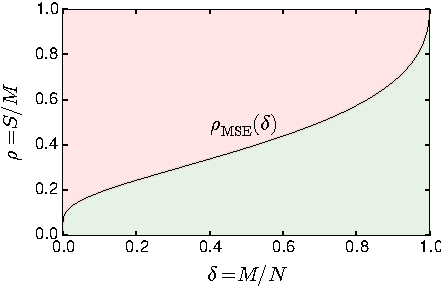
\includegraphics{l1_phase_transition}
 \caption[Phase transition for recovery of sparse solution]{\emph{Phase transition for recovery of sparse solution.} For noisy measurements $y \in \field{R}^M$ given by $y=Ax + \eta$, recovery of $S$-sparse $x \in \field{R}^N$ by is successful (mean square error is bounded) when $\rho = S/M$ is below the curve $\rho_\text{MSE}(\delta)$ shown above with $\delta = M/N$. The result holds for many types of measurement matrices $A$ and nonlinear recovery algorithms, particularly $l_1$ minimization.}
 \label{fig:l1_phase_transition}
\end{figure}%
For these results, successful recovery means that the measurement error is bounded for the worst-case noise and sparsity distributions, while failure means that the error is unbounded. The theoretical results are for the limit as $M$, $N$, and $S$ tend to infinity with fixed $(\delta, \rho)$, but simulations have shown that the transition holds for finite setups.

It must be emphasized that this phase transition represents the behavior of the \emph{optimal} recovery algorithm when faced with the parameters of the problem. The key to the success of compressed sensing is that $l_1$ minimization \emph{is} an optimal recovery algorithm; it achieves this performance with appropriate choice of the noise parameter \autocite{DT09, DMM11}. Furthermore, the optimal performance has been shown to extend empirically to other measurement ensembles \autocite{DT10, MJG+13} and theoretically to other optimization algorithms \autocite{DJM13}. Research in this area is ongoing and advancing rapidly, and it is expected that the recovery bounds and phase transition results apply to a wider class of measurement ensembles and recovery algorithms than have so far been proven. Along this line, \textcite{Str12} gives an overview of the open problems that remain to be solved.

\section{Convex Optimization}
\label{convex_optimization}
Sparse solutions to an underdetermined system of equations can be sought with a bevy of different methods. Some of these are greedy algorithms like OMP (orthogonal matching pursuit) \autocite{TG07}, some are based on statistics like AMP (approximate message passing) \autocite{DMM09}, and most are variants that improve on a basic method in some way. Of particular note are the many methods that involve a common but not universal theme: convex optimization, specifically involving minimization of the $l_1$-norm. Our focus is on methods of this type because they are easy to understand and the theory is well-established. The base case is an optimization problem known as $l_1$-regularized least squares:
\begin{equation*}\tag{$\text{P}_{\text{1}\lambda}$} \label{eq:l1rls}
 \underset{x}{\mathrm{minimize}} \quad \frac{1}{2}\norm{2}{Ax - b}^2 + \lambda\norm{1}{x}.
\end{equation*}
This problem is equivalent to basis pursuit with denoising \eqref{eq:BPDN} for a proper choice of the regularization parameter $\lambda$, but its form is more convenient for many algorithms.

\subsection{First-order Methods}
Before discussing $l_1$-regularized least squares specifically, we restrict our attention to a particular class of optimization algorithms: first-order methods. For the types of problems that we are interested in, explicit representations of the measurement matrix $A$ are not useful. The typical matrix is large and has additional structure that makes applying it via matrix multiplication inefficient. When $A$ represents convolution, a Fourier transform, or other efficient transforms as is often the case, it is much faster to compute its result using the transform operation directly. First-order optimization algorithms are interesting because they do not require using an explicit matrix representation for $A$ and $A^*$; they only require the ability to evaluate the $A$ and $A^*$ operations, which we can do efficiently even for large problem dimensions.

The most natural first-order method for minimizing a differentiable convex function $G(x)$ is gradient descent. Starting at a point $x^0$, gradient descent iteratively steps in the direction of the negative of the gradient $\grad_{G}(x) = \nabla G(x)$ until the minimum is reached.
\begin{algorithm}[H]
 \caption{Gradient Descent \autocite{Boy04}}
 \begin{algorithmic}
  \GIVEN a starting point $x^0$
  \REPEAT
  \STATE $x^{k+1} \coloneqq x^{k} - \mu \grad_{G}(x^{k})$ \COMMENT{step size $\mu$ chosen by line search}
  \UNTIL{stopping criterion is satisfied}
 \end{algorithmic}
\end{algorithm}\noindent
Gradient descent is guaranteed to converge to a minimum-value solution for smooth, convex $G(x)$ provided that the step size is chosen appropriately. This is typically done with a backtracking line search as detailed by \textcite{Boy04}. For the function $G(x) = \frac{1}{2}\norm{2}{Ax - b}^2$, the gradient is $\grad_{G}(x) = A^*(Ax - b)$. Thus in order to iteratively find the least squares solution to $Ax=b$ using gradient descent, we only need to be able to evaluate $A$ and $A^*$.

Of course, the function we want to minimize to be able to solve the $l_1$-regularized least squares problem is not differentiable, so gradient descent is not directly applicable. For non-smooth functions $F(x)$ like the $l_1$-norm, an attractive alternative to the gradient is the \emph{proximal operator}:
\begin{equation}
 \prox_{\mu F} (v) = \argmin_{x} \; \paren*{F(x) + \frac{1}{2\mu} \norm{2}{x - v}^2},
\end{equation}
where $\mu$ is a scaling factor that can be likened to a step size. The prox operator adds an $l_2$-smoothing term to a non-smooth function and outputs the vector $x$ which gives the minimum of the composite function. Using the prox operator as an iterative step in a similar manner to the gradient leads to an algorithm for minimizing non-smooth $F(x)$: the proximal point method.
\begin{algorithm}[H]
 \caption{Proximal Point \autocite{PB13}}
 \begin{algorithmic}
  \GIVEN a starting point $x^0$
  \REPEAT
  \STATE $x^{k+1} \coloneqq \prox_{\mu F}(x^{k})$ \COMMENT{scaling $\mu$ chosen by line search}
  \UNTIL{stopping criterion is satisfied}
 \end{algorithmic}
\end{algorithm}\noindent
Note that as the iterates $x^{k}$ approach the minimum $x_*$, the smoothing term goes to zero and the minimum of $F(x)$ is reached.

\subsection{Prox Operator Examples}
For many interesting functions $F(x)$, the prox operator is surprisingly easy to solve. The prox operator of the $l_1$-norm will obviously be useful, and fortunately it has a closed form solution known as soft thresholding:
\begin{equation}
 \prox_{\tau \norm{1}{x}} (v) = \soft_{\tau}(v)[k] =
    \begin{cases}
      \paren*{1 - \frac{\tau}{\abs{v[k]}}} v[k], & \abs[\big]{v[k]} > \tau\\
      0, & \abs[\big]{v[k]} \le \tau.
     \end{cases}
\end{equation}
Soft thresholding operates element-wise on a vector $v$, setting all of the elements with magnitude less than the threshold $\tau$ to zero and shrinking all other elements toward zero by $\tau$. A graphical depiction of scalar soft thresholding is given in Figure \ref{fig:soft_thresholding}.
\begin{figure}[tpb]
 \centering
 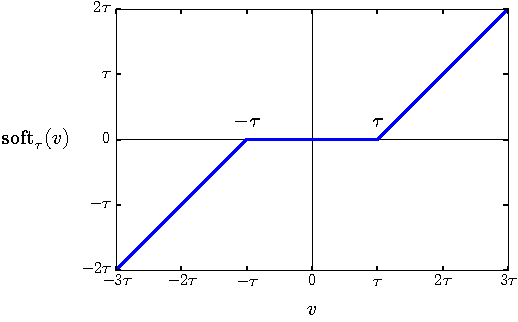
\includegraphics{soft_thresholding_function}
 \caption[Soft thresholding function]{\emph{Soft thresholding function.} The real scalar soft thresholding function evaluates to zero when the magnitude of the input is below the threshold $\tau$, and it returns a shrunken value of the input otherwise.}
 \label{fig:soft_thresholding}
\end{figure}%

The $l_2$-norm, though smooth, also has a closed form prox operator. For $F(x) = \norm{2}{x}$, the prox operator is the block soft thresholding operator,
\begin{equation}
 \prox_{\tau \norm{2}{x}} (v) = \bsoft_{\tau}(v) =
    \begin{cases}
      \paren*{1 - \frac{\tau}{\norm{2}{v}}} v, & \norm{2}{v} > \tau\\
      0, & \norm{2}{v} \le \tau.
     \end{cases}
\end{equation}
Block soft thresholding operates on the entire vector $v$, setting it to zero if its norm is less than the threshold $\tau$ and shrinking its norm to $\norm{2}{v} - \tau$ otherwise. The squared $l_2$-norm $F(x) = \frac{1}{2}\norm{2}{x}^2$ has a different prox operator called the shrinkage function:
\begin{equation}
 \prox_{\frac{\tau}{2}\norm{2}{x}^2} (v) = \shrink_{\tau}(v) = \frac{v}{1 + \tau}.
\end{equation}
In contrast to soft thresholding, the shrinkage function shrinks all of the vectors' entries by a fixed fraction defined by the scale factor $\tau$, penalizing the largest entries the most.

When the non-smooth function is the indicator $I_{\mathcal{C}}(x)$ for a closed nonempty convex set $\mathcal{C}$, which is defined as
\begin{equation}
 I_{\mathcal{C}}(x) = \begin{cases}
                       0, & x \in \mathcal{C}\\
                       +\infty, & x \notin \mathcal{C},
                      \end{cases}
\end{equation}
the prox operator acts as Euclidean projection onto $\mathcal{C}$:
\begin{equation}
 \prox_{I_{\mathcal{C}}} (v) = \argmin_{x} \; \paren*{I_{\mathcal{C}}(x) + \frac{1}{2} \norm{2}{x - v}^2} = \argmin_{x \in \mathcal{C}} \; \norm{2}{x - v} = \Pi_{\mathcal{C}}(v).
\end{equation}
When viewed in this way, prox operators can be seen as generalized projections. In the case of the $l_1$-norm, soft thresholding "projects" onto a sparse space enforced by the $l_1$-norm by setting small elements to zero. Practically, indicator functions are useful for enforcing constraints in optimization problems. By adding an appropriate indicator function to the objective, solutions can be required to lie in the corresponding convex set. For example, if a solution to an underdetermined system is known to have a particular sparsity pattern, the indicator function for the locations of the zeros can be added to a least squares objective to solve for the closest solution with that sparsity pattern.

\subsection{Proximal Gradient}
With the necessary operators in place, we finally return to the problem of $l_1$-regularized least squares \eqref{eq:l1rls}. This is a problem of the form
\begin{equation}
 \underset{x}{\mathrm{minimize}} \quad F(x) + G(Ax - b),
\end{equation}
where $F(x)$ is (possibly non-differentiable) function with a known prox operator $\prox_{F} (v)$, $A$ is a linear operator, $b$ is a vector constant, and $G(z)$ is a differentiable function so that the gradient of the second term is $A^* \grad_{G}(Ax - b)$. With the split smooth and non-smooth objective, we can imagine a two-step iteration stage that first steps in the gradient direction of the smooth term and then evaluates the prox operator of the non-smooth term. This leads to an optimization algorithm known as the proximal gradient method.
\begin{algorithm}[h]
 \caption{Proximal Gradient \autocite{PB13}}
 \begin{algorithmic}
  \GIVEN a starting point $x^0$, a step size $0 < \mu \le 2/L$
  \REPEAT
  \STATE $z^{k+1} \coloneqq x^k - \mu \, A^* \grad_{G}(Ax^k - b)$
  \STATE $x^{k+1} \coloneqq \prox_{\mu F}(z^{k+1})$
  \UNTIL{stopping criterion is satisfied}
 \end{algorithmic}
\end{algorithm}\\
Stopping criteria for the algorithm vary, but we will choose one based on the residual of the optimality condition $0 \in \partial F(x_*) + \nabla_x G(Ax_* - b)$. This residual for the iterate $x^{k+1}$ is given by
\begin{equation}
 r^{k+1} = \frac{1}{\mu}\paren*{x^k - x^{k+1}} + A^*\paren*{\grad_G(Ax^{k+1} - b) - \grad_G(Ax^k - b)}.
\end{equation}
The algorithm is said to have converged if $\norm{2}{r^{k+1}}$ is small, less than a tolerance threshold. The basic proximal gradient method also uses a fixed step size $\mu > 0$, and to guarantee convergence it must satisfy $\mu \le 2/L$ where $L$ is the global Lipschitz constant of the gradient of $G(Ax - b)$. For all $x$, $\tilde{x}$ in the domain of $\nabla_x G$, the gradient is globally Lipschitz continuous if
\begin{equation}
 \norm{2}{\nabla_x G(Ax - b) - \nabla_x G(A\tilde{x} - b)} \le L \norm{2}{x - \tilde{x}}.
\end{equation}

One interpretation of the proximal gradient method is as a majorization-minimization algorithm. At every step, the algorithm majorizes (upper bounds) the objective and then minimizes the majorization. In this case, the majorization involves taking a first-order approximation of the smooth portion of the objective and adding a trust region penalty:
\begin{equation}
 G_{\mu}(x, \tilde{x}) = G(\tilde{x}) + \innerprod*{\nabla_x G(A\tilde{x} - b)}{x - \tilde{x}} + \frac{1}{2\mu}\norm{2}{x - \tilde{x}}^2.
\end{equation}
Then for $\mu \le 1/L$, we have the majorization
\begin{equation}
 F(x) + G(Ax - b) \le F(x) + G(x^{k}) + \innerprod*{\nabla_x G(Ax^{k} - b)}{x - x^{k}} + \frac{1}{2\mu}\norm{2}{x - x^{k}}^2
\end{equation}
about the point $x^{k}$. Minimizing the majorization is just a simple call to the prox operator of $F$:
\begin{align}
 x^{k+1} &= \argmin_{x} \; \paren*{F(x) + G(x^{k}) + \innerprod*{\nabla_x G(Ax^{k} - b)}{x - x^{k}} + \frac{1}{2\mu}\norm{2}{x - x^{k}}^2}\nonumber\\
 &= \argmin_{x} \; \paren*{F(x) + \frac{1}{2\mu}\norm{2}{x - \paren*{x^{k} - \mu \, A^* \grad_G(Ax^k - b)}}}\nonumber\\
 &= \prox_{\mu F}\paren*{x^{k} - \mu \, A^* \grad_G(Ax^k - b)}.
\end{align}
This step is precisely the one taken in the proximal gradient method.

Proximal gradient applied to the $l_1$-regularized least squares problem has a special name: iterative soft thresholding. If we divide the objective as $F(x) = \lambda\norm{1}{x}$ and $G(z) = \frac{1}{2}\norm{2}{z}$, the proximal operator $\prox_{F}(x) = \soft_{\lambda}(x)$ is soft thresholding, the gradient $\grad_{G}(z) = z$ is the identity, and the method takes the explicit form given in Algorithm \ref{alg:ist}.
\begin{algorithm}[H]
 \caption{Iterative Soft Thresholding}
 \label{alg:ist}
 \begin{algorithmic}
  \GIVEN a starting point $x^0$, a step size $0 < \mu \le 2/\norm{2}{A}^2$
  \REPEAT
  \STATE $z^{k+1} \coloneqq x^k - \mu \, A^*(Ax^k - b)$
  \STATE $x^{k+1} \coloneqq \soft_{\mu \lambda}(z^{k+1})$
  \UNTIL{stopping criterion is satisfied}
 \end{algorithmic}
\end{algorithm}\noindent
Clearly the iterative soft thresholding method is aptly named. With the form of the gradient known, we also know that its Lipschitz constant $L$ is given by $\norm{2}{A}^2$, the squared induced $l_2$-norm of the matrix $A$. If $A$ is scaled so that its norm is unity, then the maximum fixed step size that guarantees convergence is $2$.

\subsection{Improvements on Proximal Gradient}
The proximal gradient method can be improved both theoretically and in practice through the use of an acceleration term and a variable step size. Acceleration of first-order methods is based on the work of \textcite{Nes83, Nes88} for smooth objectives, which was extended by \textcite{BT09, BT10} to the proximal gradient method. \textcite{Nes07} also adapted acceleration to the case of a composite objective, but that particular approach requires multiple evaluations of the prox operator per step. Acceleration works by adding an appropriate ratio of the prior iterate to the current iterate before executing the gradient and prox steps, thus this simple modification improves convergence without significantly increasing per-step computation. More recently, \textcite{OC13} found that an adaptive restart scheme for the acceleration term improves convergence in practice even more significantly. Applied to the $l_1$-regularized least squares problem, the accelerated method is known as FISTA, or the fast iterative soft thresholding algorithm \autocite{BT09}.

A variable step size is the other modification that practically improves performance. Though convergence is guaranteed by bounding the steps by the global Lipschitz constant, such steps can be too conservative when the gradient's curvature is locally variable. When this is the case, even a standard backtracking line search for the step size is not sufficient since it can only decrease the step size. Both \textcite{SGB11} and \textcite{BCG11}, apparently independently, suggested an expansive backtracking line search scheme to accommodate increasing the step size if warranted. With this scheme, the step size is increased by a constant factor after every iteration; convergence is assured by checking the majorization condition at the next iterate and backtracking on the step size by a constant factor if necessary. Though backtracking results in repeated application of $A$, $A^*$, and the gradient and prox operators, the typical net result is fewer computations and faster convergence. With both the acceleration and variable step size enhancements, we get a proximal gradient method that significantly improves upon the performance of the basic method. The accelerated proximal gradient method, with adaptive restart and adaptive step size, is detailed as Algorithm \ref{alg:accelproxgrad}.
\begin{algorithm}[tpb]
 \caption{Accelerated Proximal Gradient, with adaptive restart and adaptive step size}
 \label{alg:accelproxgrad}
 \begin{algorithmic}
  \GIVEN starting point $x^0$
  \GIVEN initial step size $\mu^0 > 0$, step expansion factor $\alpha > 1$, backtracking factor $0 < \beta < 1$
  \GIVEN tolerance $\epsilon > 0$
  \STATE $x^{-1}, w^0 \coloneqq x^0$
  \STATE $g^0 \coloneqq A^* \grad_{G}(Aw^0 - b)$

  \STATE $t^0 \coloneqq 1$
  \STATE $\mu^1 = \mu^0$
  \STATE $\gamma \coloneqq 1$
  
  \REPEAT
   \IF {$\innerprod*{w^k - x^k}{x^k - x^{k-1}} > 0$}
    \STATE $t^k \coloneqq 1$
   \ENDIF
   \REPEAT
    \STATE $t^{k+1} \coloneqq \paren*{1 + \sqrt{1 + 4\paren*{t^k}^2 \gamma}}/2$
    \STATE $\theta \coloneqq \paren*{t^k - 1}/t^{k+1}$
    \STATE $w^{k+1} \coloneqq x^k + \theta \paren*{x^k - x^{k+1}}$
    \STATE
    \STATE $g^{k+1} \coloneqq A^* \grad_{G}\paren*{Aw^{k+1} - b}$
    \STATE $x^{k+1} \coloneqq \prox_{\mu^{k+1} F}\paren*{w^{k+1} - \mu^{k+1} \, g^{k+1}}$
    \STATE
    \IF {$G(Ax^{k+1} - b) \le G(Aw^{k+1} - b) + \innerprod*{x^{k+1} - x^k}{g^{k+1}} + \frac{1}{2\mu^{k+1}}\norm{2}{x^{k+1} - w^{k+1}}^2$}
     \STATE \textbf{break}
    \ELSE
     \STATE $\mu^{k+1} \coloneqq \beta \mu^{k+1}$
     \STATE $\gamma \coloneqq \mu^{k} / \mu^{k+1}$
    \ENDIF
   \UNTIL
   \STATE $r^{k+1} \coloneqq \paren*{x^k - x^{k+1}}/\mu^{k+1} + g^{k+1} - g^k$
   \IF {$\norm{2}{r^{k+1}} \le \epsilon$}
    \STATE \textbf{break}
   \ENDIF
   \STATE $\mu^{k+1} \coloneqq \alpha \mu^{k+1}$
   \STATE $\gamma = \mu^k / \mu^{k+1}$
  \UNTIL
 \end{algorithmic}
\end{algorithm}%

\subsection{Related Prox Methods}
Naturally, there are other algorithms that solve the same (or a similar) split objective optimization problem and even make use of the prox operator. While proximal gradient requires part of the objective, $G(z)$, to be differentiable, these additional methods work in the more general case where only an easily-evaluated prox operator is required for each of the split-objective terms. Since this is a less-restrictive requirement, these methods are primarily of interest due to their broader applicability. Depending on the exact problem being solved, however, it is certainly possible for them to outperform even the accelerated proximal gradient method.

The alternating direction method of multipliers (ADMM) algorithm, also known as Douglas-Rachford splitting, solves the problem
\begin{equation}
 \underset{x}{\mathrm{minimize}} \quad F(x) + G(x)
\end{equation}
where both $F$ and $G$ have prox operators given by $\prox_{F}(x)$ and $\prox_{G}(x)$. Notice that this definition does not include the affine transformation $Ax - b$ as with the proximal gradient method. The ADMM algorithm is similar to proximal gradient in that it splits the iteration into two steps, first applying $\prox_{F}(x)$ and then applying $\prox_{G}(x)$ as detailed in Algorithm \ref{alg:admm}. Amazingly, the algorithm converges for any positive value of the penalty parameter $\rho$. ADMM can vary in its exact form depending on which order the prox operators are applied or, equivalently, by how the objective is split and assigned to the two functions, so care must be taken to choose the optimal formulation for a given problem. A detailed treatment of ADMM, including per-iteration adjustment of the penalty parameter to help improve convergence, is given by \textcite{BPC+11}.
\begin{algorithm}[tpb]
 \caption{Alternating Direction Method of Multipliers (ADMM)}
 \label{alg:admm}
 \begin{algorithmic}
  \GIVEN starting point $x^0$ with dual $y^0$, penalty parameter $\rho > 0$
  \STATE $u^0 \coloneqq \rho y^0$
  \STATE $z^0 \coloneqq \prox_{\rho G}\paren*{x^0 + u^0}$
  \REPEAT
   \STATE $x^{k+1} \coloneqq \prox_{\rho F}\paren*{z^k - u^k}$
   \STATE $z^{k+1} \coloneqq \prox_{\rho G}\paren*{x^{k+1} + u^k}$

   \STATE $r^{k+1} \coloneqq x^{k+1} - z^{k+1}$
   \STATE $s^{k+1} \coloneqq \paren*{z^k - z^{k+1}}/\rho$

   \STATE $u^{k+1} \coloneqq u^k + r^{k+1}$
  \UNTIL{$\norm{2}{r^{k+1}}$ and $\norm{2}{s^{k+1}}$ are small}
 \end{algorithmic}
\end{algorithm}%

Linearized ADMM, also called the Split Inexact Uzawa method \autocite{EZC10}, is a variant of ADMM that includes an affine transformation in the objective function with a matrix $A$ and vector $b$:
\begin{equation}
 \underset{x}{\mathrm{minimize}} \quad F(x) + G(Ax - b),
\end{equation}
where again $F$ and $G$ are not necessarily differentiable and have prox operators $\prox_{F}(x)$ and $\prox_{G}(z)$. It is not trivial to accommodate an affine transformation when evaluating the prox operator of most functions, so the explicit inclusion here is significant in practice and the reason linearized ADMM is often used over the original. Our version of linearized ADMM, given in Algorithm \ref{alg:admmlin}, is based on the one described by \textcite{PB13}. However, ours is unique because it includes not only a penalty adjustment scheme adapted from the ADMM method of \textcite{BPC+11} but also a novel expansive backtracking line search for the step size $\mu$. In fact, the interpretation of the $\mu$ parameter as a step size is unique, and doing so allows us to adapt the majorization condition and line search scheme used in the accelerated proximal gradient algorithm (Algorithm \ref{alg:accelproxgrad}) for use with linearized ADMM. We have not formally analyzed the convergence of linearized ADMM including these modifications or rigorously proved their benefits, but they do result in significant improvement in practice in a manner similar to the corresponding proximal gradient method schemes. As a point of reference, we have found that an expansion factor of $\alpha=1.25$, a backtracking factor of $\beta=0.5$, a maximum residual gap of $\gamma=10$, and a penalty factor of $\rho=1.5$ are the most effective parameters for a variety of problems.
\begin{algorithm}[tpb]
 \caption{Linearized ADMM}
 \label{alg:admmlin}
 \begin{algorithmic}
  \GIVEN starting point $x^0$ with dual $y^0$
  \GIVEN step size $\mu > 0$, step expansion factor $\alpha > 1$, backtracking factor $0 < \beta < 1$
  \GIVEN penalty parameter $\rho > 0$, maximum residual gap $\gamma > 1$, penalty factor $\tau > 1$
  \GIVEN penalty freezing index $k_{\rho_\text{max}}$
  \STATE $u^0 \coloneqq \rho y^0$
  \STATE $u^{-1} \coloneqq u^0$
  \REPEAT
   \REPEAT
    \STATE $x^{k+1} \coloneqq \prox_{\mu F}\paren*{x^k - \frac{\mu}{\rho} A^*\paren*{2u^k - u^{k-1}}}$
    \IF {$\mu \norm{2}{A\paren*{x^{k+1} - x^k}}^2 \le \rho \norm{2}{x^{k+1} - x^k}^2$}
     \STATE \textbf{break}
    \ELSE
     \STATE $\mu \coloneqq \beta \mu$
    \ENDIF
   \UNTIL
   \STATE $z^{k+1} \coloneqq \prox_{\rho G}\paren*{Ax^{k+1} - b + u^k}$

   \STATE $r^{k+1} \coloneqq Ax^{k+1} - b - z^{k+1}$

   \STATE $u^{k+1} \coloneqq u^k + r^{k+1}$
   
   \STATE $s^{k+1} \coloneqq A^*\paren*{u^{k+1} - u^k}/\rho + A^*\paren*{u^{k-1} - u^k}/\rho + \paren*{x^k - x^{k+1}}/\mu$
   
   \IF {$k < k_{\rho_\text{max}}$}
    \IF {$\norm{2}{r^{k+1}} > \gamma \norm{2}{s^{k+1}}$}
     \STATE $\rho = \rho/\tau$
     \STATE $u^{k+1} = u^{k+1}/\tau$
     \STATE $u^k = u^k/\tau$
    \ENDIF
    \IF {$\norm{2}{s^{k+1}} > \gamma \norm{2}{r^{k+1}}$}
     \STATE $\rho = \rho\tau$
     \STATE $u^{k+1} = u^{k+1}\tau$
     \STATE $u^k = u^k\tau$
    \ENDIF
   \ENDIF
   
   \IF {$\norm{2}{A\paren*{x^{k+1} - x^k}} \ne 0$}
    \STATE $\mu \coloneqq \alpha \rho \frac{\norm{2}{x^{k+1} - x^k}^2}{\norm{2}{A\paren*{x^{k+1} - x^k}}^2}$
   \ENDIF
  \UNTIL{$\norm{2}{r^{k+1}}$ and $\norm{2}{s^{k+1}}$ are small}
 \end{algorithmic}
\end{algorithm}%

The final algorithm of interest actually embodies a class of algorithms that include linearized ADMM as a special case: the primal dual hybrid gradient (PDHG) method. It solves the same problem as linearized ADMM, although that problem is sometimes written in the form
\begin{equation}
 \min_{x} \; \sup_{y} \; F(x) + \innerprod*{y}{Ax - b} - G^*(y),
\end{equation}
where $G^*$ denotes the convex conjugate function of $G$. The conjugate function is defined as
\begin{equation}
 G^*(y) = \sup_{x} \; \innerprod*{y}{x} - G(x),
\end{equation}
and since $(G^*)^* = G$, the equivalence between the two minimization problems is clear. Writing the objective in this alternative form makes it clear that the primal and dual objectives are near-mirror images, and it gives the algorithm a beautiful symmetry as shown in Algorithm \ref{alg:pdhg}. Equivalence to the basic linearized ADMM algorithm comes when the acceleration parameters are constant with $\theta_p = 0$ and $\theta_d = 1$. This relationship between the two methods, and the other forms of the PDHG method, are explored in detail by \textcite{EZC10}. The generality of the PDHG algorithm is attractive, but unfortunately that generality is a negative when it comes to achieving performance on par with the other prox methods. Although we have not included adaptive parameter selection in our PDHG formulation, such improvements do exist; \textcite{GEB13} detail one possible scheme.
\begin{algorithm}[tpb]
 \caption{Primal dual hybrid gradient (PDHG)}
 \label{alg:pdhg}
 \begin{algorithmic}
  \GIVEN starting point $x^0$ with dual $y^0$
  \GIVEN primal step size $\gamma_p > 0$, dual step size $\gamma_d > 0$
  \GIVEN primal acceleration factor $0 \le \theta_p^0 \le 1$, dual acceleration factor $0 \le \theta_d^0 \le 1$
  \STATE $y^{-1} \coloneqq y^0$
  \REPEAT
   \STATE $\bar{y}^k \coloneqq y^k + \theta_d^k \paren*{y^k - y^{k-1}}$
   \STATE $\hat{x}^{k+1} \coloneqq x^k - \gamma_p A^*\paren*{\bar{y}^k}$
   \STATE $x^{k+1} \coloneqq \prox_{\gamma_p F}\paren*{\hat{x}^{k+1}}$
   \STATE $\bar{x}^{k+1} \coloneqq x^{k+1} + \theta_p^k \paren*{x^{k+1} - x^k}$
   \STATE $\hat{y}^{k+1} \coloneqq y^k + \gamma_d \paren*{A\bar{x}^{k+1} - b}$
   \STATE $y^{k+1} \coloneqq \prox_{\gamma_d G^*}\paren*{\hat{y}^{k+1}}$
   \STATE $p_{k+1} \coloneqq \paren*{x^k - x^{k+1}}/\gamma_p - A^*\paren*{y^k - y^{k+1}} - \theta_d^k A^*\paren*{y^k - y^{k-1}}$
   \STATE $d_{k+1} \coloneqq \paren*{y^k - y^{k+1}}/\gamma_d - \theta_p^k A\paren*{x^k - x^{k+1}}$
  \UNTIL{$\norm{2}{p^{k+1}}$ and $\norm{2}{d^{k+1}}$ are small}
 \end{algorithmic}
\end{algorithm}%

\subsection{Similar Convex Problems}
\label{similar_convex_problems}
With the additional prox-based algorithms, we can solve other $l_1$-minimization problems that might be of interest. Depending on convergence performance in specific instances, some of the problems described in this section may even be preferable. The first problem is already a familiar one, and it is equivalent to $l_1$-regularized least squares for an appropriate choice of the noise parameter $\epsilon$: basis pursuit with denoising. Instead of a regularization term, the noise constraint is explicit:
\begin{equation*}\tag{$\text{P}_{\text{1}\epsilon}$}
 \begin{matrix*}[l]
  \underset{x}{\mathrm{minimize}} & \norm{1}{x}\\
  \text{subject to} & \norm{2}{Ax - b} \le \epsilon.
 \end{matrix*}
\end{equation*}
In this form, the meaning of the noise constraint is easier to understand and to adapt to particular use cases. Unfortunately, we lose the ability to use proximal gradient methods: BPDN can be solved using linearized ADMM or PDHG by letting $F$ represent the $l_1$-norm and $G$ represent the indicator for the $l_2$-ball of radius $\epsilon$.

The Dantzig selector problem replaces the $l_2$ noise constraint with an $l_\infty$ noise constraint:
\begin{equation*}\tag{$\text{P}_{\text{1}\delta}$}
 \begin{matrix*}[l]
  \underset{x}{\mathrm{minimize}} & \norm{1}{x}\\
  \text{subject to} & \norm{\infty}{A^*(Ax - b)} \le \delta,
 \end{matrix*}
\end{equation*}
where $\norm{\infty}{v} = \max_k \abs*{v[k]}$. Like the prior estimators, the Dantzig selector is suitable for finding a sparse solution in accordance with the theory of compressed sensing. This problem was originally proposed by \textcite{CT07}, and they did so for two reasons that both relate to the application of $A^*$ to the residual term $Ax - b$ in the noise constraint. The first reason is that it makes the noise constraint invariant to orthonormal transformations applied to the residual. The second reason is that it ensures that no elements of the solution's residual remain highly correlated with the model dictionary. With the $l_2$ noise constraint, it is possible for significant model-correlated components of the residual to remain if they are small in magnitude. Although these two properties are desirable, the form of the Dantzig selector requires an extra application of $A$ and $A^*$ per iteration when compared to the other problems, and that cost can be significant. The Dantzig selector can be solved using linearized ADMM or PDHG by letting $F$ represent the $l_1$-norm and having $G$ represent the indicator for the $l_\infty$-ball of radius $\delta$.

Tibshirani's original LASSO (least absolute shrinkage and selection operator) estimator \autocite{Tib96} flips the optimization problems we've seen thus far on their heads, instead minimizing the squared residual and constraining the $l_1$-norm:
\begin{equation*}\tag{$\text{P}_{\text{2}\tau}$}
 \begin{matrix*}[l]
  \underset{x}{\mathrm{minimize}} & \frac{1}{2}\norm{2}{Ax - b}^2\\
  \text{subject to} & \norm{1}{x} \le \tau.
 \end{matrix*}
\end{equation*}
This problem is not to be confused with other problems commonly called the LASSO, whereby either $l_1$-regularized least squares or basis pursuit is meant. The LASSO is particularly useful when solved repeatedly for different values of the $l_1$-norm constraint $\tau$. By doing so in sequence from low to high $\tau$, one can observe a family of solutions with different levels of sparsity while taking advantage of the efficiency gained by reusing the prior solution to speed convergence of the subsequent optimization. Statistical selection techniques can then be used to pick the most appropriate solution out of the family, perhaps based on a sudden change in the form of the solutions. The LASSO can be solved using proximal gradient, linearized ADMM, or PDHG by letting $F$ represent the indicator of the $l_1$-ball of radius $\tau$ and having $G$ represent half the squared $l_2$-norm.

Finally, the zero-constrained least squares problem is useful when the sparsity pattern of the solution is known:
\begin{equation*}\tag{$\text{P}_{\text{2z}}$}
 \begin{matrix*}[l]
  \underset{x}{\mathrm{minimize}} & \frac{1}{2}\norm{2}{Ax - b}^2\\
  \text{subject to} & x \in \mathcal{Z},
 \end{matrix*}
\end{equation*}
where $\mathcal{Z}$ represents the set of vectors with a particular zero pattern. This situation can arise when one seeks to de-bias the solution of another sparse estimator. Because the $l_1$-norm tends to shrink all solutions, it produces estimates that are biased toward zero. To remove this bias, one can take the zero locations discovered by the minimum $l_1$-norm solution and use them to find an unbiased sparse solution via zero-constrained least squares. This problem can be solved using proximal gradient, linearized ADMM, or PDHG by letting $F$ represent the indicator of the zero set $\mathcal{Z}$ and having $G$ represent half the squared $l_2$-norm.
\graphicspath{{chapters/waveform_inversion/figures/}}
\chapter{Waveform Inversion Method}
\label{waveform_inversion}
In the quest to eliminate matched filter sidelobes from decoded radar data, we have developed a model that represents the radar scene as discrete reflectivity coefficients $h[n,p]$ in a delay-frequency space:
\begin{equation}
 y[m] = \sum_{p=0}^{P-1} \sum_{n=0}^{N-1} s[Rm-p+L-1] e^{2 \pi i n(Rm-p+L-1)/N} h[n,p],
\end{equation}
written compactly as
\begin{align}
 y = \sqrt{N} A h \quad \Leftrightarrow \quad y = A x.
\end{align}
Solving for the reflectivity coefficients from the measured signal $y$ provides a sidelobe-free and potentially higher-resolution ($R > 1$) radar scene. The primary barrier is that the model represents an underdetermined system of equations with infinite solutions.

We have already encountered the least-norm solution: the matched filter result. Recall that for the radar model, the composed operator $AA^*$ is the identity scaled by the $l_2$ norm of $s$, which we can choose to be 1 without loss of generality. Thus, the least-norm solution is given by equation \eqref{eq:least_norm_solution} as
\begin{equation}
 x_{l_2} = A^*y,
\end{equation}
which is just the (scaled) matched filter bank applied to the measured signal. Just as the least-norm solution to a general underdetermined system may not always be the most appropriate, in this case we already know that the simple linear method provides an inadequate solution.

Fortunately, one of the reasons we sought a delay-frequency representation of the radar scene is that we expect such a representation to be sparse. With the delay-frequency radar model, measurement incoherence is completely determined by the choice of transmission waveform $s$, although it remains to be seen which values for $s$ will result in minimal coherence. Provided that the measurements described by the radar model are sufficiently incoherent, the theory of compressed sensing says that we can recover the true sparse signal using convex optimization algorithms like the proximal gradient method. In this chapter, we bring these ideas to bear on the radar problem and detail how to implement them to perform waveform inversion.

\section{Related Work}
\label{related_work}
\subsection{Other Radar Applications}
Sparse approximation and the radar problem are a natural match, and researchers have proposed applying compressed sensing to radar almost since the theory was first developed \autocite{BS07}. Some applications are concerned only with acquiring the returned radar signal at lower cost or with a higher sampling rate. In this case, the signal is undersampled with respect to the Nyquist rate and compressed sensing is performed in the truest sense of the term. Theory specific to this problem, with the sparse signal represented in an overcomplete and thus coherent dictionary, is examined by \textcite{CENR11}. On the practical side, \textcite{YTN+12} demonstrate wideband compressed sensing of radar pulse parameters, with the recovery done completely in hardware. The potential for compressed sensing to reduce radar hardware complexity and cost is also noted by \textcite{BS07} and \textcite{End10}. This research is interesting because of its potential to completely replace existing receivers with ones that are both cheaper and higher-bandwidth, but it is almost completely orthogonal to the problem of coded waveform ambiguity.

The role of sparsity in radar signal processing and the relationship between compressed sensing techniques and established processing methods is discussed by \textcite{PEPC10}, but their focus is on imaging with synthetic aperture radar. \textcite{HM13} simulate a related technique, compressed sensing interferometric imaging, and apply it to observe equatorial spread-F using the Jicamarca ISR. Their results compare favorably to the existing Capon's method and maximum entropy techniques. Radar imaging applications also exhibit waveform ambiguity and would benefit in theory from the elimination of sidelobes, but these and other methods safely ignore the sidelobe problem by either working with stationary targets and using a chirp waveform (\autocite{PEPC10}) or using short uncoded pulses (\autocite{HM13}). Because of this, the existing imaging techniques are more akin to compressed sensing tomography than to waveform inversion.

\subsection{Theoretical Support}
Two works focusing on the time-frequency representation problem do have direct relevance to waveform inversion. \textcite{BSN08} propose using a representation similar to our radar model for learning the parameters of communication channels, while \textcite{HS09} explore the use of compressed sensing for increased resolution of radar target detection using nearly the same model. Both are complementary to our work because they focus on waveform selection and theoretical conditions for sparse recovery rather than the practical details of applying the technique to real data. Consequently, it is useful to know that their measurement matrices have the restricted isometry property when the transmitted waveform is given by a random binary code \autocite{BSN08} or the Alltop sequence \autocite{HS09}, the latter of which is a type of discrete quadratic chirp.

A number of authors address the compressed sensing problem for general convolutional sensing matrices, again either with random codes \autocite{TWD+06, BHR+07, Rom09, PR10} or with the Alltop sequence \autocite{PR10}. The specifics vary, but all prove measurement incoherence and show that sparse recovery is guaranteed with a number of measurements on the order of the solution sparsity. These results establish specific forms of the general incoherent sampling theorem from Chapter \ref{sparsity_background}. The differences between these models and ours are minor but notable, so the recovery guarantees are not directly applicable. All of the existing literature is based on a dense measurement matrix, which can only be produced by an exceptionally long pulse relative to the delay window size. As a result, the typical measurement incoherence of our model is reduced, and we can expect to require either more measurements or higher sparsity for success. Nevertheless, we are justified theoretically in seeking sparse recovery with measurements of this form.

\section{Solution Procedure}
\label{waveform_inversion_solution}
With incoherent measurements of the form $y=Ax$ and an assumed sparse $x$, we are primed to solve an $l_1$-minimization problem to recover $x$. In reality, radar data has noise, so the measurements are more accurately approximated by
\begin{equation}
 y = Ax + \eta,
\end{equation}
where $\eta$ represents a vector of i.i.d.\ zero-mean complex Gaussian noise. To ensure that $A$ is properly scaled with $\norm{2}{A} = 1$ and that any noise has the same average power after applying the adjoint (matched filter) $A^*$, we normalize the code $s$ so that $\norm{2}{s} = 1$. Of the sparse recovery problems that include measurement noise, we will focus on $l_1$-regularized least squares because of its simplicity and generally quick convergence. In the notation of our model, this problem solves the following:
\begin{equation*}\tag{$\text{P}_{\text{1}\lambda}$}
 \underset{x}{\mathrm{minimize}} \quad \frac{1}{2}\norm{2}{Ax - y}^2 + \lambda\norm{1}{x}.
\end{equation*}
Choosing the regularization parameter $\lambda$ is crucial since it balances the importance of finding a sparse solution with the importance of minimizing deviation from the measurements.

\subsection{Regularization Parameter}
The solution is expected to deviate from the measurements due to noise, and it is through quantifying the noise that we can choose an appropriate $\lambda$. It is common practice to estimate the noise variance $\hat{\sigma}^2$ by averaging the power of presumed noise-only samples $y_\eta$:
\begin{equation}
 \hat{\sigma}^2 = \frac{1}{K} \sum_{k=0}^{K-1} \abs*{y_{\eta}[k]}^2,
\end{equation}
where $K$ is the number of noise samples. The noise measurement is usually acquired separately from the data measurement (or perhaps each is a different segment of a continuous stream of samples), and it typically corresponds to large delays/ranges for which no target backscatter is assumed. It can also be helpful to stabilize the noise estimate by averaging it across multiple pulses, provided one can assume that the noise power is fixed over some period of time. Certainly it makes sense to use a single noise estimate when analyzing a slice of data that encompasses multiple pulses, if only so that slight changes in the estimate do not cause apparent changes in signal-to-noise ratio (SNR) that might be interpreted instead as signal variance. No matter how the noise power estimate $\hat{\sigma}^2$ is made, accuracy is important since the estimate is used to determine the regularization parameter.

To set the regularization parameter $\lambda$, we use a property of the solution $x_*$ to \eqref{eq:l1rls}:
\begin{equation}\label{eq:optimality_condition}
 \norm{\infty}{A^*\paren*{Ax_* - y}} \le \lambda,
\end{equation}
In words, every entry of the result of applying $A^*$ to the residual must have a magnitude less than $\lambda$. This fact is evident from the objective's first-order optimality condition from subdifferential calculus:
\begin{equation}
 0 \in \partial \paren*{\frac{1}{2}\norm{2}{Ax - y}^2 + \lambda\norm{1}{x}}\bigg|_{x = x_*},
\end{equation}
which evaluates to
\begin{equation}
 \paren*{A^*\paren*{Ax_* - y}}_i \in \begin{cases}
                                      \set{\lambda {x_*}_i/\abs*{{x_*}_i}}, & \abs*{{x_*}_i} > 0\\
                                      \set{\lambda : \abs{\lambda} \le 1}, & {x_*}_i = 0
                                     \end{cases}
\end{equation}
for every individual entry ${x_*}_i$ of $x_*$. One possible choice for $\lambda$ is just below the critical value $\lambda_\text{crit} = \norm{\infty}{A^*y}$ at which $x = 0$ ceases to be the optimal solution. The choice of $\lambda = 0.99\lambda_\text{crit}$ or $\lambda = 0.95\lambda_\text{crit}$ provides a maximally sparse nonzero solution, but it can allow the residual $y - Ax_*$ to have a higher variance than would be expected with a given noise level.

Since we have an estimate for the noise power, we can do better. As was shown with the derivation of the radar model, $A^*$ scaled by $\sqrt{N}$ is equivalent to matched filtering. Therefore, we can think of $\sqrt{N} A^*\paren*{Ax_* - y}$ as the matched filter applied to the residual. In order for $x_*$ to be an acceptable solution, we restrict the filtered residual so that its entries have a magnitude less than the noise level. Otherwise, we would consider that element to represent scattered signal from a target, which should be represented in the solution $x_*$ instead of in the residual. Since $\sqrt{N} \lambda$ is an upper bound on the filtered residual from equation \eqref{eq:optimality_condition}, $\lambda$ specifies the detection threshold. For a given false alarm rate for detection, we can set the detection threshold at a fixed multiple $C_\text{FAR}$ of the noise power. In other words, we want to set a solution constraint of
\begin{equation}
 \norm{\infty}{\sqrt{N} A^*\paren*{Ax_* - y}}^2 \le N\lambda^2 = C_\text{FAR} \hat{\sigma}^2,
\end{equation}
which implies that we want
\begin{equation}
 \lambda = \sqrt{C_\text{FAR}} \frac{\hat{\sigma}}{\sqrt{N}}.
\end{equation}
If the noise is truly zero-mean complex Gaussian, then $C_\text{FAR} = 4$ corresponds to a false alarm rate of about $2\%$. Targets with an SNR less than $4$ (after the sidelobes from higher-signal targets are removed) won't be included in the solution, and about $2\%$ of the noise will be included in the solution. This is a reasonable trade-off between detection and model complexity, so our default value for $\lambda$ is $2\hat{\sigma}/\sqrt{N}$.

\subsection{Iterative Thresholding Matched Filter}
One method for recovering the sparse solution for the reflectivity coefficients is to use the iterative soft thresholding algorithm derived from the proximal gradient method.
\begin{algorithm}
 \caption*{\textbf{Algorithm \ref{alg:ist}} Iterative Soft Thresholding}
 \begin{algorithmic}
  \GIVEN a starting point $x^0$, a step size $0 < \mu \le 2/\norm{2}{A}^2$
  \REPEAT
  \STATE $z^{k+1} \coloneqq x^k - \mu \, A^*(Ax^k - y)$
  \STATE $x^{k+1} \coloneqq \soft_{\mu \lambda}(z^{k+1})$
  \UNTIL{stopping criterion is satisfied}
 \end{algorithmic}
\end{algorithm}%
Examining the steps of this algorithm leads to an intuitive interpretation, in radar terminology, of the nonlinear procedure for arriving at a sparse solution. We describe this interpretation as an \emph{iterative thresholding matched filter}.

Consider the algorithm's first step for an initial guess of $x^0 = 0$ and step size $\mu = 1$:
\begin{equation}
 z^1 \coloneqq A^*y.
\end{equation}
In radar terms, this first step is to apply the matched filter to the received signal. The next step produces a first "guess" of the solution by thresholding the matched filter result:
\begin{equation}
 x^1 \coloneqq \soft_{\lambda}(z^1) = \soft_{\lambda}(A^*y).
\end{equation}
Values in the matched filter result that are below the detection threshold set by $\lambda$ are set to zero, and the remaining values are shrunk toward zero. In other words, the first guess is simply everything that the matched filter would classify as a detected signal, which can include sidelobes.

Looping to the next iteration, the third step is:
\begin{equation}
 z^2 \coloneqq x^1 + A^*(y - Ax^1).
\end{equation}
The interpretation is that the expected received signal based on the first guess is calculated and compared to the actual measurement. The difference is matched filtered to see what newly-revealed components of the signal were left out the first time, and that result is added to the original guess. As before, the fourth step thresholds the matched filter result to get an improved guess:
\begin{equation}
 x^2 \coloneqq \soft_{\lambda}(z^2) = \soft_{\lambda}\paren*{A^*\paren*{x^1 + A^*(y - Ax^1)}}.
\end{equation}
Further iterations proceed in the same manner, applying matched filtering and thresholding to steadily improve the solution estimate until convergence.

\subsection{Scaling and Noise}
It is convenient to work in terms of $x$ so that the model operations $A$ and $A^*$ are well-scaled, but $h = x / \sqrt{N}$ is what we actually want given that the matched filter bank has the scaling $\sqrt{N}A^*y$. The reflectivity coefficients $h$ are indeed the matched filter result with modeled sidelobes and the filtered residual removed:
\begin{align}
 \sqrt{N} A^*y &= \sqrt{N} A^*\paren*{y - Ax + Ax}\nonumber\\
 &= N A^*Ah + \sqrt{N} A^*\paren*{y - Ax}\nonumber\\
 \underbrace{\sqrt{N} A^*y}_\text{matched filter} &= h + \underbrace{\paren*{NA^*A - I}h}_\text{sidelobes} + \underbrace{\sqrt{N} A^*\paren*{y - Ax}}_\text{matched filtered residual}\label{eq:sidelobe_removal}.
\end{align}
Recall that the operation $N \cdot A^*A$ adds matched filter ambiguity to its input (equation \ref{eq:ambiguity_AstarA}), hence subtracting the identity $I$ and applying it to $h$ leaves only the sidelobes generated from $h$. The residual mostly represents measurement noise, but a significant part of it is the bias that is left after $l_1$-minimization overly-shrinks the solution toward zero.

Solution bias can be a problem if it is not handled properly. One method to acquire an unbiased estimate is to find the least-squares solution with the sparsity pattern that matches $x_*$. This can be solved efficiently using any of the prox methods detailed in Chapter \ref{sparsity_background}. With reasonable false-alarm rates, however, the sparsity pattern of $x_*$ will include noise coefficients, and this de-biasing step can cause those coefficients to take on unreasonable values in an effort to match all of the noise. Fortunately for this application, the de-biasing step is generally unnecessary since in most cases we can work with a modified solution that includes the residual term. If all we want to do is remove sidelobes from the matched filter solution, then we can subtract only that term from equation \eqref{eq:sidelobe_removal} and define
\begin{align}
 \hat{h}_* &= h_* + \sqrt{N} A^*\paren*{y - Ax_*},\\
\intertext{or equivalently}
 \hat{h}_* &= \frac{x_*}{\sqrt{N}} + \sqrt{N} A^*\paren*{y - Ax_*}.
\end{align}
This modified reflectivity estimate $\hat{h}_*$ nicely encapsulates the entire solution. The first term is the sparse reflectivity, embodying the signal that is well-represented by the radar model. The second term is matched filtering applied to the residual, embodying everything that is not captured by the radar model. If the sparse solution leaves out significant components that fall below the noise threshold, those signals will be visible in the residual term. Instead of calling everything in the residual "noise" and discarding it, we incorporate it into the solution and let it be judged on its own merits.

\subsection{Solution Residual}
Care must be taken when working with the residual for purposes other than comparison to the full delay-frequency matched filter result. Since waveform inversion eliminates sidelobes, there is a new viable option for representing the solution as a range-time-intensity (RTI) plot: totaling the reflected power across all frequencies and displaying it as a function of range and time. In other words, we sum the square magnitude of the reflectivity over the frequency index and plot that instead of a single-frequency slice. Doing this with the estimate $\hat{h}_*$ produces incorrect results since the noise is not independent across frequency. The residual values $\zeta = y - Ax_*$ are independent, but the matched filtered residual across delay-frequency space is clearly not. Summing across the frequency index of $A^*\zeta$ is acceptable, and it produces the zero-frequency matched filter result of correlating $\zeta$ with the transmitted waveform $s^*$. The problem arises from the added scaling factor of $\sqrt{N}$ in the residual term of $\hat{h}_*$, which magnifies the noise by that factor after frequency summing. Therefore, when calculating a frequency-integrated RTI plot, we drop the scaling factor on the residual term and proceed as normal.

It must be noted that adding the residual to the sparse solution in the manner of $\hat{h}_*$ does not produce a solution that matches the measurements exactly. A nearly-sparse exact solution $x_0$ of $y=Ax$ is given by adding the unscaled residual to $x_*$:
\begin{equation}
 x_0 = x_* + A^*\paren*{y - Ax_*}.
\end{equation}
This solution is nearly-sparse because it has few nonzero values with magnitude greater than $\lambda$, but many nonzero values with magnitude less than $\lambda$. Applying the forward model produces
\begin{align}
 Ax_0 &= Ax_* + AA^*\paren*{y - Ax_*}\nonumber\\
 &= Ax_* + y - Ax_*\nonumber\\
 &= y
\end{align}
since $AA^*$ is the identity. Though the scaled solution $h_0 = x_0/\sqrt{N}$ is an unbiased estimate of the true reflectivity coefficients, it is not particularly useful. One negative is that it is not exactly sparse, but the difference is small enough to be of almost no importance. The main problem with $h_0$ is that it spreads the residual out over delay-frequency space in a manner that masks its true representation in the measurement space. The noise coefficients $x_\eta = A^*\paren*{y - Ax_*}$ that get added to $x_*$ are simply the least-norm estimate for $y - Ax_* = Ax_\eta$, which has no physical meaning. In order to understand where the model fails in approximating the true solution, it is preferable to work with the estimate $\hat{h}_*$ since it can be compared directly to the matched filter result.

\section{Implementation}
\label{waveform_inversion_implementation}
Performing waveform inversion in practice requires the ability to calculate the radar model and solve a sparse approximation problem using it. Obviously there was no existing computer code that implemented our specific radar model, so that had to be written from scratch. As for sparse approximation, many packages are freely available that solve the various forms of that problem. However, many of them do not accommodate specifying $A$ and $A^*$ as functional operators rather than explicit matrices, so that leaves far fewer software packages to choose from. The \pkg{TFOCS} package described by \textcite{BCG11} and available at \url{http://cvxr.com/tfocs/}\nocite{tfocs} is the only one that implements the algorithms in Chapter \ref{sparsity_background} and includes the performance enhancements that speed convergence. The initial exploration of sparse approximation using the radar model was done using \pkg{TFOCS}, and it was well-suited to that purpose.

Unfortunately, two obstacles were encountered. The first is that it was difficult to tune the algorithm parameters to achieve reliably good performance. The second is that \pkg{TFOCS} is written using MATLAB, which became a problem when we decided to implement the radar model in Python for ease of reuse. In the end, it was necessary to also code all of the convex optimization algorithms from scratch. To prevent this from happening to other researchers in the future, the radar model and proximal operator software packages have been made available as BSD-licensed open source Python code \autocite{python2_7, Oli07}, which can be found on GitHub at \url{http://github.com/ryanvolz}. The radar model package was given the creative name of \pkg{radarmodel}, while the proximal optimization routines are packaged together as \pkg{prx}. For the purposes of reproducibility, all of the code for producing the results in this thesis is also available at the same GitHub site. Special recognition must go to the developers of \pkg{matplotlib} \autocite{matplotlib} and \pkg{IPython} \autocite{ipython}; their plotting and interactive programming tools have made this work possible.

\subsection{\pkg{radarmodel}}
The \pkg{radarmodel} package implements the forward operator $A$ and adjoint operator $A^*$, which are necessary to compute solutions using the radar model of Chapter \ref{radar_model}.  Users first specify the transmission code $s$, the undersampling ratio $R$, the length of the measurement vector $M$, and the number of frequency steps $N$ for a particular problem formulation. Then, the program creates tailored functions for the forward and adjoint operators which can be used to quickly compute those operations repeatedly. As with most scientific computing in Python, \pkg{radarmodel} makes extensive use of the \pkg{numpy} package \autocite{numpy} for fast array computations.

Since the primary goal in writing special-purpose functions to compute the radar model is to make them as fast and efficient as possible, great care was taken in implementing and benchmarking the operators. Multiple formulations that deconstruct the operations into different convolution, Fourier transform, and array arithmetic steps were tested, and \pkg{radarmodel} can select the best formulation for a particular set of problem parameters on the fly. The different formulations all make use of the FFT operator through the \pkg{pyffw} package \autocite{pyfftw}, and some of them use the compiled-language add-ons provided by \pkg{cython} or \pkg{numba}. The \pkg{cython} package \autocite{cython} allows one to take a restricted form of the Python language, add static declarations, and compile it into C code. The \pkg{numba} package \autocite{numba} allows one to decorate customized \pkg{numpy} routines and compile them just-in-time (JIT) by dynamically invoking the \pkg{llvm} compiler. Both packages provide optimized performance for intensive calculations without having to leave Python, greatly easing development and debugging. The result is a radar model implementation that is one or two orders of magnitude faster and less memory-intensive than a naive or matrix implementation.

\subsection{\pkg{prx}}
The \pkg{prx} package implements the proximal gradient, accelerated proximal gradient, ADMM, linearized ADMM, and PDHG methods for solving a number of $l_1$-minimization problems. It also provides functions for computing the prox operators that are necessary to solve those problems. As with \pkg{radarmodel}, \pkg{prx} makes extensive use of the \pkg{numpy} package \autocite{numpy}. Each optimization algorithm requires the user to specify the objective functions $F$ and $G$, the linear operators $A$ and $A^*$, the data vector $b$, and algorithm parameters for step size and convergence tolerance. The optimization algorithms can be used to solve any problem with the correct split-objective form, provided that $F$ and $G$ can be specified. These objective functions can be composed from a selection of elemental functions with known gradients and/or prox operators, or entire standard problems like $l_1$-regularized least squares can be solved using specialized functions. The package is designed to be easily-extensible so that if a new objective function is required, it can be implemented in a standard form and used with the optimization routines just like the standard functions. This design has proven effective in testing a variety of algorithms and optimization problems, including ones not originally envisioned.

In contrast to the \pkg{radarmodel} package, the key to efficient computation with \pkg{prx} lies in optimizing the individual algorithms and making them easy to use. All of the enhancements mentioned in Chapter \ref{sparsity_background}, and a few additional ones, are included so that the algorithms converge as quickly as possible. Moreover, all of the required tuning parameters can be specified if required, but the default values work well enough that tuning won't be necessary in most cases. Since the package is written completely in Python, it is easy to examine and modify the code to figure out what is happening behind the scenes, making the implementation far more useful than a computational black box. Special care was taken to provide user-visible documentation that describes each of the optimization routines, gradient and proximal operators, and standard problem formulations in detail, with references included if more information is required. 

\subsection{Algorithm Comparison}
With a variety of proximal optimization algorithms available to solve the $l_1$-regularized least squares problem, it was necessary to test each algorithm to determine which converges fastest in general when applied with the radar model. Computation time for all of these algorithms is dominated by the evaluation of the forward and adjoint operators of the radar model, so the primary interest is in minimizing the number of iterations required for convergence. Table \ref{tab:prox_alg_comparison} lists the iteration count until convergence for some of the algorithms detailed in Chapter \ref{sparsity_background} and implemented in the \pkg{prx} package. All of the algorithms were applied to the same instance of an $l_1$-regularized least squares problem using the radar model provided by the \pkg{radarmodel} package. The required single pulse of radar data came from the Jicamarca ISR using a minimum peak sidelobe waveform, and it contained scattering from a meteor head echo. Convergence was determined using the same absolute and relative tolerance parameters for all of the algorithms. Regardless of these details, the results are generally descriptive of our experience using these algorithms on actual radar data.
\begin{table}
 \renewcommand{\arraystretch}{1.2}
 \caption[Convergence comparison of proximal optimization algorithms]{\emph{Convergence comparison of proximal optimization algorithms.} The tables list the number of steps until convergence (and backtracking steps, if applicable) for the same instance of $l_1$-regularized least squares.}
 \label{tab:prox_alg_comparison}
 \begin{subtable}[t]{0.4\textwidth}
  \centering
  \caption{Proximal gradient variations}
  \label{tab:proximal_gradient}
  \begin{tabular}{@{}ll@{}}
   \toprule
   Method & Iterations\\
   \midrule
   Proximal gradient & 4463\\
   $+$ Acceleration & 2915\\
   $+$ Adaptive restart & 399\\
   $+$ Adaptive step & 51 (36)\\
   $-$ Acceleration & 58 (27)\\
   \bottomrule
  \end{tabular}
 \end{subtable}%
 \begin{subtable}[t]{0.6\textwidth}
  \centering
  \caption{Three different methods}
  \label{tab:prox_algorithms}
  \begin{tabular}{@{}ll@{}}
   \toprule
   Method & Iterations\\
   \midrule
   Accelerated proximal gradient & 51 (36)\\
   Linearized ADMM (adaptive) & 79 (96)\\
   PDHG (fixed step) & 4466\\
   \bottomrule
  \end{tabular}
 \end{subtable}
\end{table}%

Table \ref{tab:proximal_gradient} compares the proximal gradient method with its improvements, each version adding a feature to the last. The unmodified proximal gradient algorithm is somewhat slow to converge, while the accelerated scheme is about a third faster. Adding adaptive restart of the acceleration term brings a significant improvement, dropping the number of steps down an order of magnitude. Adding the adaptive step size scheme drops the number of steps by another order of magnitude, converging in less than a hundred total steps (complete steps and partial backtracking steps). Finally, keeping the adaptive step size but dropping the acceleration scheme just barely increases the number of iterations over the accelerated version, with even fewer backtracks. Because of this vast improvement from step size adjustment, it seems that the radar model coupled with $l_1$-regularized least squares is particularly prone to large variations in the optimal step size. This would appear to be an exceptional requirement, since as far as we are aware, an expanding adaptive step size is included in only one of the available proximal gradient implementations (\pkg{TFOCS}), and it is not well-publicized in the literature. Also of note is how the acceleration scheme only becomes really effective once adaptive restart is allowed, but even that improvement is inconsequential compared to having an adaptive step size.

The accelerated and fully adaptive proximal gradient method is compared to linearized ADMM and PDHG in Table \ref{tab:prox_algorithms} (plain ADMM is not applicable to this $l_1$-regularized least squares problems because of the affine transformation). Given that both linearized ADMM and PDHG can handle more general problems, it is not surprising that they both take longer to converge than the optimized proximal gradient method. The linearized ADMM method uses an adaptive step size scheme of our own devising that is similar to that for the proximal gradient method. Considering the importance of the adaptive step for the latter method, it is no wonder that linearized ADMM converges much faster than the fixed step PDHG. The PDHG algorithm used here is the basic one; it can be improved with adaptive parameter selection, but that implementation was deemed unnecessary for now given the relative success of the proximal gradient method. It is interesting, and probably not a coincidence, that both of the fixed step algorithms (PDHG and basic proximal gradient) converge in almost the same number of iterations. This fact not only shows how closely-related all of these algorithms are, but it also emphasizes just how step-size dependent this problem is.

Limited performance testing was also done for the basis pursuit with denoising and Dantzig selector problems, with both using the linearized ADMM algorithm. Approximately equivalent sparse answers can be achieved with appropriate parameter selection, but both algorithms require more iterations to converge than $l_1$-regularized least squares. Roughly speaking, basis pursuit with denoising takes about twice as many iterations, while the Dantzig selector takes about ten times as many iterations. Little effort has been put into investigating optimal algorithm parameters for these problems, so it is likely that performance can be improved. Nevertheless, it is unlikely that either will be able to converge faster than $l_1$-regularized least squares using the accelerated proximal gradient method. Given the success of that combination, we feel justified in continuing to use it almost exclusively.
\graphicspath{{chapters/experimental_results/figures/}}
\chapter{Experimental Results}
\label{experimental_results}
The real value in using sparsity for waveform inversion manifests through its application. Backed by an efficient implementation of the radar model operators and the quick convergence of tuned sparse recovery algorithms, we are primed to demonstrate the waveform inversion method on real radar data. Though the eventual goal in applying this technique is to enable highly-flexible and artifact-free measurements, the goals of this experiment are to \begin{inparaenum}[(1)]
 \item show that waveform inversion produces results that are consistent with our expectations,
 \item directly compare the effectiveness of different waveforms, and
 \item collect high-quality meteor data.
\end{inparaenum}

We expected that inversion would eliminate delay-frequency sidelobes and strictly improve upon matched filtering, and the experiment is successful in demonstrating that. We know that the pulse waveform directly affects measurement incoherence in terms of compressed sensing, and the experiment shows that successful inversion is dependent on the compactness of the peak of the waveform's ambiguity function. Regarding meteors, the hope was that eliminating sidelobes and increasing resolution through waveform inversion would allow us to address the open questions concerning flares and micrometeoroid fragmentation \autocite{MBMC10}. Further experimentation will be required to answer those questions, but the experiment proves that the technique is still useful for eliminating interference between meteor head echoes and stationary targets like non-specular trails and the equatorial electrojet. Without sidelobe interference, each of those phenomena can be detected more reliably and studied independently.

From February 28 through March 2, 2011, we collected approximately 48 hours of nearly-continuous data observing the equatorial ionosphere using the Jicamarca 50 MHz radar. That amounted to over two terabytes of receiver samples. Even with fast code and good algorithms, it is not reasonable at this time to apply the waveform inversion technique to anything more than tiny segments of that data. We have chosen to focus on a handful of examples collected from the Jicamarca data set in order to analyze them in detail and infer the method's effectiveness in general. With the knowledge gained from this experience, we are able make recommendations to aid future applications of the waveform inversion technique.

\section{Jicamarca}
\label{jicamarca_overview}
The Jicamarca 50 MHz radar is a phased array composed of 18,432 crossed half-wave dipoles in a 96 by 96 square grid (Figures \ref{fig:jicamarca} and \ref{fig:jicamarca_and_me}), covering an area of almost 85,000 square meters.
\begin{figure}[tbp]
 \centering
 %\includegraphics[width=0.75\textwidth,trim=0px 20px 0px 100px,clip]{fairuse/jicamarca}
 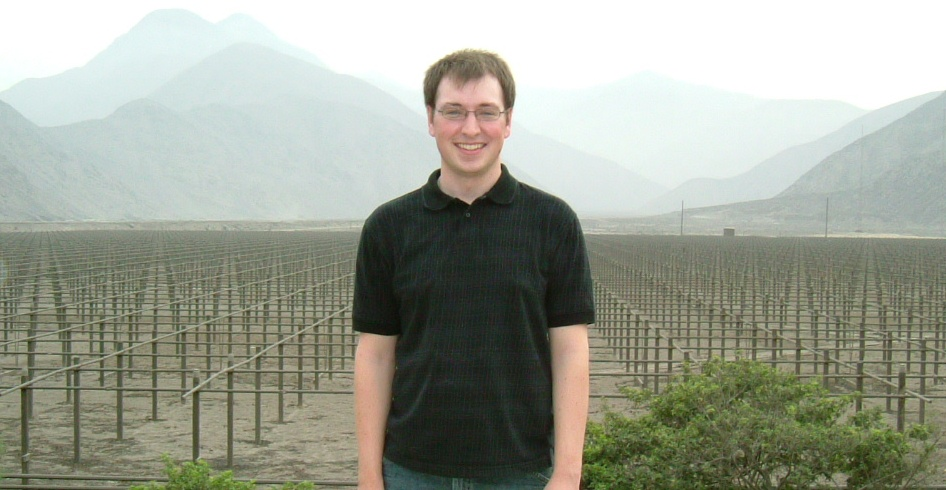
\includegraphics[width=0.75\textwidth]{jicamarca_and_me}
 \caption[The Jicamarca 50 MHz radar]{\emph{The Jicamarca 50 MHz radar.} The author is pictured, pre-experiment, in front of the Jicamarca Radio Observatory's main radar, a large phased array operating at 50 MHz and consisting of 18,432 crossed half-wave dipoles. Located outside of Lima, Peru, the radar's primary use is to study the equatorial ionosphere from its vantage point near the magnetic equator.}
 \label{fig:jicamarca_and_me}
\end{figure}%
It is located inland from Lima, Peru, at a geographic latitude and longitude of 11.95$^\text{o}$ south, 76.87$^\text{o}$ west, placing it near the magnetic equator \autocite{Och63}. Accordingly, the main use of Jicamarca is the study of the equatorial ionosphere, and monitoring its background plasma through incoherent scatter is one primary objective. Since the radar is able to point perpendicular to the Earth's magnetic field (or nearly so), it enjoys a number of rare capabilities. Ultra-precise measurement of ionospheric electric fields is one benefit of that configuration, as is the ability to view field aligned irregularities, which are frequently fueled by meteor ionization and radar-visible as non-specular meteor trails \autocite{WH69, CK94}. The study of these and other unique transient events, including spread-F and the equatorial electrojet, is another focus of Jicamarca's scientific program. Thanks to the radar's low VHF frequency relative to other high-power large-aperture (HPLA) radars, more meteor head echoes are detectable with the Jicamarca array than with almost all of those other HPLAs given the inverse scaling of frequency with received signal strength, which scales approximately as $1/f^2$. Head echoes, trails, and electrojet are near-constant features of the daytime ionosphere at Jicamarca. This crowded and challenging environment is a great proving ground for new measurement techniques, and it provides a surfeit of opportunities for testing our waveform inversion method.

\subsection{Specifications}
The observatory is currently equipped with three transmitters that each have a peak power output of about 1.5 MW, for a total possible transmitter power of 4.5 MW. The transmitter system supports a variety of pulsed waveforms, including binary-phase codes and the LFM chirp. These pulses can be transmitted with a maximum duty cycle of 6\%, a maximum bandwidth of about 1 MHz (shortest pulse of 1 microsecond), and a maximum length of 2 milliseconds. Four phase-coherent receivers can be used to sample the acquired signal with a maximum bandwidth of 1 MHz. Each receiver downmixes the signal to baseband frequency and outputs complex samples representing in-phase and quadrature components \autocite{JICAMARCA_SPEC}.

\subsection{Array Segmentation}
The four receiver channels can measure signals from distinct subsets of the whole array. One typical configuration involves sampling the four quadrants of the array independently. Comparison of signal phase between these quadrants through interferometry allows one to determine the signal's direction of arrival. The channels can also be used to sample independent polarizations or more complex interferometry setups with multiple measurement baselines. The dipoles are actually organized into 64 separate, square modules; the modules can be sampled in any combination, but they can also be phased independently to form different beam patterns. Tuned appropriately, the full array has a one-way half power beamwidth (full-width at half maximum) of 1.1$^\text{o}$ and can be electronically steered within about 7$^\text{o}$ of zenith. Currently, individual module phasing must be carried out manually by adjusting cable lengths, but a computer-controlled phasing system is being developed to enable pulse-to-pulse beam pointing \autocite{JICAMARCA_SPEC}.

\section{Setup}
The suitability of different radar waveforms for sparse recovery is an open question. We expect from theoretical results that random or pseudorandom waveforms will produce suitably incoherent measurements, but most of the standard waveforms also merit investigation. Because they are designed to minimize the effects of ambiguity, codes with ideal sidelobe properties are likely to also be useful for inversion. Our experiment using the Jicamarca radar was designed to test the effectiveness of a number of these common waveforms by comparing them side-by-side while scattering from the same targets. Switching the code on a pulse-to-pulse basis allows us to judge waveforms against each other under the same circumstances. As long as we eventually repeat the same waveform after a short time relative to the persistence of the target, we can build up equivalent views of a radar scene using a number of different waveforms.

\subsection{Waveforms}
For this experiment, we selected five different waveforms and stepped through them sequentially before repeating the sequence. The five waveforms are depicted using a meteor head and trail in Figure \ref{fig:waveform_sequence}; the waveforms are, in order, a Barker-13 code (B$_\text{13}$), a minimum peak sidelobe code (MSL$_\text{51}$), an uncoded pulse, a linear frequency modulation (LFM) chirp, and a pseudorandom code (PSRND$_\text{51}$).
\begin{figure}[tpb]
 \centering
 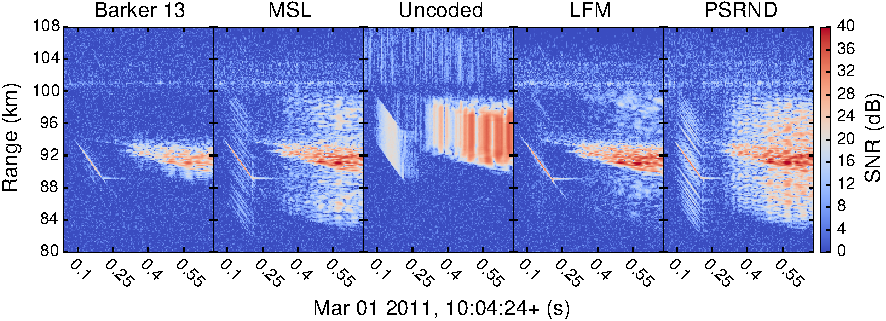
\includegraphics{head_and_flare_mf_rti_block}
 \caption[Sequence of waveforms used in the Jicamarca experiment]{\emph{Sequence of waveforms used in the Jicamarca experiment.} The images show example meteor data collected with the Jicamarca radar using five different pulse waveforms. The radar transmits just one of the five waveforms with each pulse, stepping through the sequence of five in the order shown before repeating.}
 \label{fig:waveform_sequence}
\end{figure}%
The first four were chosen because they are widely used for collecting meteor head echo and trail data \autocite{WPW96, ELWF01, MBMH08, COHD02}. The pseudorandom code was chosen because it was expected to have good waveform inversion performance based on compressed sensing theory \autocite{BSN08, PR10}. The three binary phase codes are described by the following sequences:
\begin{align}
 s_{\text{B}_\text{13}} &= 1111100110101\nonumber\\
 s_{\text{MSL}_\text{51}} &= 000111000111111100010001100100010010101001001001011\nonumber\\
 s_{\text{PSRND}_\text{51}} &= 011111000010000001001100001011000001001011010011100\nonumber.
\end{align}

\subsection{Pulse Parameters}
With the exception of the uncoded pulse, a bandwidth of 1 MHz (the maximum at Jicamarca) was fixed as the primary design point. A high bandwidth equates to better pulse compression and smaller regions of ambiguity. For the phase-coded pulses, that requirement specifies a baud length of 1 $\mu$s. For the LFM chirp, it specifies a total frequency sweep of 1 MHz, centered around the radar frequency. The Barker-13 code is the longest binary code with a maximum sidelobe level of 1 when the peak is normalized to the code length, but it is still short, with a total pulse length of 13 $\mu$s, compared to the other pulses. We wanted a longer minimum peak sidelobe code in order to test the effects of pulse length, so the code of length 51 was chosen since it is the longest that has a peak sidelobe level of 3 or less. Hence, the MSL$_\text{51}$ pulse has a length of 51 $\mu$s. The lengths of the LFM and pseudorandom pulses were chosen to match the minimum sidelobe pulse. The pseudorandom code was indeed produced by a random number generator; we drew a few binary codes of length 51 until we found one with a somewhat-uniform autocorrelation. Finally, the uncoded pulse bears almost no relation to the others. It was included as a baseline so that any unusual results from the coded pulses could be compared to the simplest data possible. A length of 40 $\mu$s was arbitrarily chosen to be long enough for reasonable sensitivity but short enough for reasonable ambiguity, and it is close to the value used by \textcite{MDW+03} at Arecibo.

\subsection{Pulse Timing}
Meteors are typically observed at altitudes ranging from 80 to 120 kilometers, although they are sometimes observed as low as 70 kilometers and as high as 140 kilometers. With that as our primary range window of interest, we chose an inter-pulse period of 1.02 ms, with the corresponding maximum unambiguous range of 153 km, to minimize the time required to repeat the waveform sequence. It is advantageous to repeat each waveform as quickly as possible to ensure that even transient events would be sampled sufficiently by each type of pulse. This is also the reason that the waveform sequence was limited to five pulses. With that inter-pulse period, the longest pulses in our pulse sequence nearly achieve the maximum duty cycle of Jicamarca's transmitter.

\subsection{Sampling}
High resolution is an obvious goal for meteor measurements so that accurate range and range rate estimates are possible. Waveform inversion is also dependent on having enough measurements relative to the sparsity level to ensure success. The highest sampling rate is desirable, and at Jicamarca that means a sampling period of 1 $\mu$s. With the selected waveforms consuming 1 MHz of bandwidth and switching phases at a period of 1 $\mu$s, no other choice would have made sense.

\section{Procedure}
\label{waveform_inversion_procedure}
The waveform inversion procedure specified in Section \ref{waveform_inversion_solution} was applied to second-long windows of the Jicamarca data. To ensure proper normalization for inversion, the radar model was defined with the code sequence $s$ normalized to a power of 1. To ensure that the number of frequency steps exceeded the length of the longest code sequences, the number of frequency steps $N$ was set at 128. Specifying a power of 2 ensures maximally-efficient Fourier transforms, and the higher value ensures just enough frequency resolution to differentiate moving head echoes from stationary targets. Except where noted, the model was defined with no undersampling, $R=1$. In all cases, we used the accelerated proximal gradient method with adaptive restart and adaptive step size to iteratively solve for the sparse reflectivity from the measurements. Each pulse was analyzed individually, with no shared information other than the uniformly-specified regularization parameter $\lambda$, which was set based on the estimated noise level. Using a recent laptop computer to perform the computations, the solution for each one-second segment of data took anywhere from 15 minutes to 1 hour to calculate. For a single pulse, the solution converged in approximately 1 second, with denser solutions taking correspondingly longer.

\section{Pseudorandom Pulse Results}
\label{pseudorandom_results}
Given the theoretical backing, it was expected that the pseudorandom waveform would be suitable for inversion. Fortunately, that is the case. Many of the waveform inversion features of the pseudorandom code are shared by the other waveforms. Therefore, we can summarize many of the basic features of the technique by first limiting our attention to the pseudorandom pulses.

\subsection{Pulse Slices}
Figures \ref{fig:head_timeslice} and \ref{fig:trail_timeslice} compare waveform inversion and matched filter bank results over a series of individual pseudorandom pulses.
\begin{figure}[tpb]
 \centering
 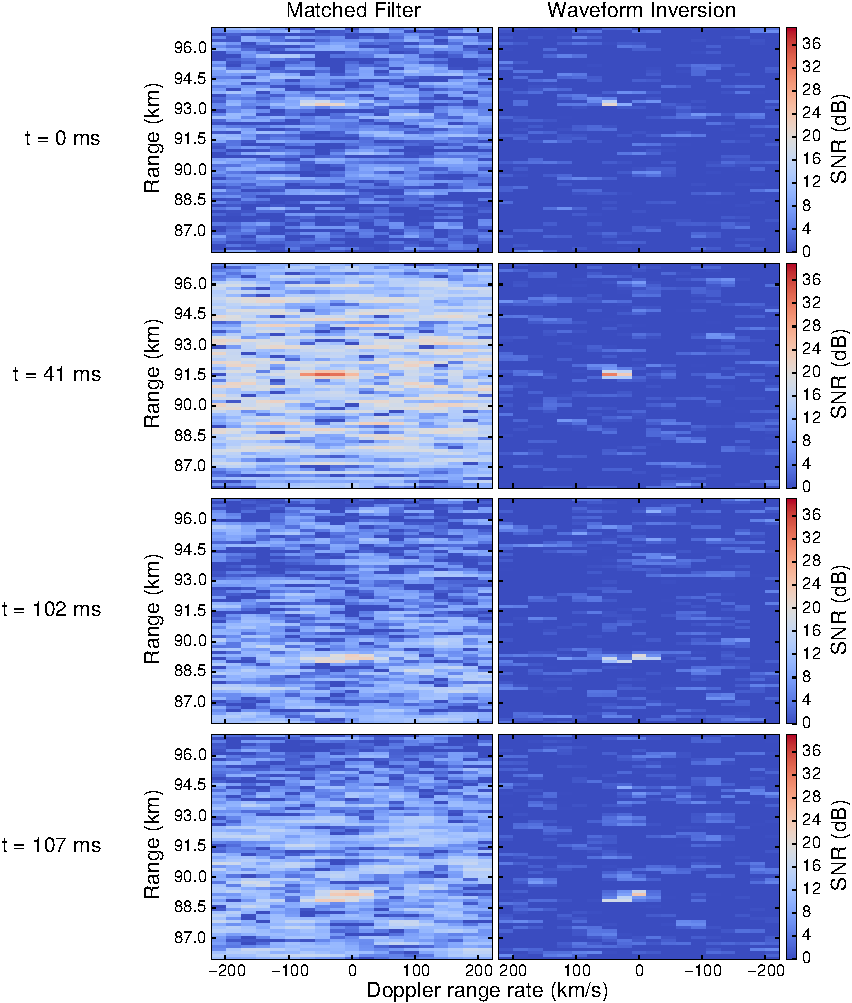
\includegraphics{head_and_flare_mf_vs_recovered_p4_ts20}
 \caption[Pulse slices comparing matched filter and waveform inversion]{\emph{Pulse slices comparing matched filter and waveform inversion.} The images in each row depict meteor head echo scattering as a function of range (delay) and Doppler range rate (frequency) for a single pseudorandom pulse. Corresponding pulse times, relative to the first pulse, are shown at left. The differentiated signal in the waveform inversion result (right column), somewhat obscured in the matched filter result (left column), shows the head echo descending in range and flaring.}
 \label{fig:head_timeslice}
\end{figure}%
\begin{figure}[tpb]
 \centering
 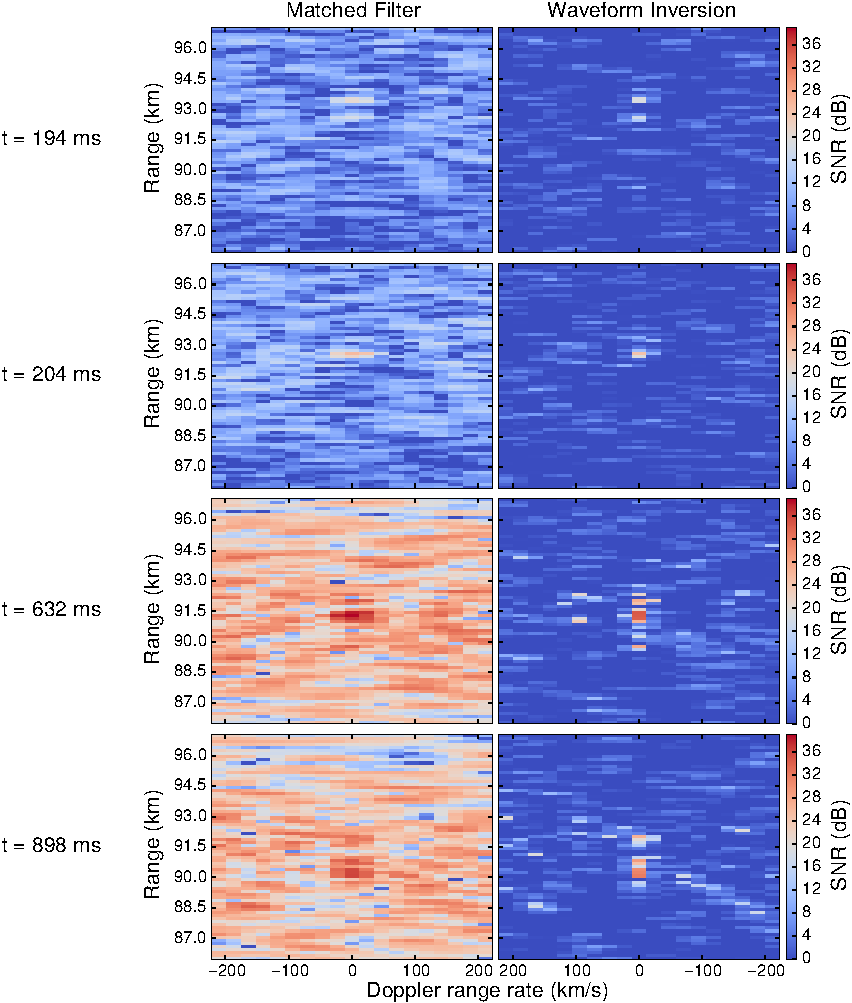
\includegraphics{head_and_flare_mf_vs_recovered_p4_ts52}
 \caption[Pulse slice comparison for a meteor trail]{\emph{Pulse slice comparison for a meteor trail.} The images in each row depict non-specular trail scattering as a function of range (delay) and Doppler range rate (frequency) for a single pseudorandom pulse. Corresponding pulse times, relative to the time of the first pulse shown in Figure \ref{fig:head_timeslice}, are shown at left. Waveform inversion (right column) removes the sidelobes obscuring the matched filter result (left column) to make the fluctuating scattering at zero-range rate clearly visible.}
 \label{fig:trail_timeslice}
\end{figure}%
Each slice represents data from a single pulse and shows part of the delay-frequency decomposition of the radar signal, giving SNR as a function of range and Doppler range rate. Figure \ref{fig:head_timeslice} shows the time evolution of a meteor head echo that ends in a flare. The head echo is first visible as a single point with negative range rate coming toward the radar, and over time it descends in range until flaring and exiting the radar beam. Figure \ref{fig:trail_timeslice} depicts the initial appearance and later fluctuation in the non-specular trail that follows the head echo. The scattering has a Doppler range rate of zero and fades in and out over the ranges containing the meteor plasma, according to the scattering characteristics of the evolving field-aligned irregularities.

The range rate axis has particularly poor resolution for these and all of the other results. The meteor head echo, traveling at approximately 40 km/s toward the radar, is only two range rate/frequency steps away from zero out of the 128 total grid points. This is a result of Jicamarca's relatively low baseband frequency of 50 MHz. At that frequency, even fast moving targets can barely generate a significant frequency shift relative to the available pulse lengths. Better frequency/range rate resolution is only possible by increasing the length of time covered by the frequency analysis, and that means analyzing the same target over multiple pulses. As such, the frequency resolution cannot be improved without the development of a multi-pulse waveform inversion technique.

Though it makes no practical difference for a single point target like the meteor head echo, the first thing to notice from the results is just how significant the delay-frequency sidelobes are in the matched filter solution. Waveform inversion effectively eliminates those sidelobes, leaving only the head echo points and noise, the latter of which has been added back to the sparse solution from the residual. It is also important to note the second row of head echo images, in which the solitary target appears to occupy multiple points spanning two range rate bins. This is as expected for a point target, due to the blurring experienced as a result of discretization (see Section \ref{point_target_reflectivity}). The true range rate lies between those two grid points, and the discrete model copes by spreading the signal over both. The flaring seen in the last two rows of head echo images is notable because sidelobe removal allows us a clearer view of the signal, which can be seen spreading to zero range rate while the head echo continues to descend. Given the poor frequency resolution, it is impossible to draw any conclusions from this result, but it is a good illustration of a potential future application.

The non-specular meteor trail is most notable for how the results go from completely cluttered in the matched filter case to relatively clean in the waveform inversion case, all thanks to the elimination of sidelobes. The most significant scattering is still noticeable with the matched filter, but it is also impossible to tell if the rest represents actual scattering or just delay-frequency sidelobes. Waveform inversion answers that question by clearly separating true scattering from sidelobe. Nevertheless, the waveform inversion solution is not perfect. It includes some significant signal at impossibly high frequencies/range rates, which we are inclined to identify as reconstruction artifacts. The best guess is that the artifacts represent the result of the transmitted signal not exactly matching the ideal, infinite-bandwidth code used in the model. As a result, the sparse solution is forced to include whatever coefficients add together to make up the difference between the actual and expected pulse shape. Imperfect matching is sufficient for good pulse compression, but the difference is much harder to account for in the sidelobes.

\subsection{Integrated RTI Plots}
The same meteor head echo, flare, and trail is shown in Figure \ref{fig:mf_vs_recovered_rti} as a range-time-intensity (RTI) plot.
\begin{figure}[tpb]
 \vspace{-1.5\baselineskip}
 \begin{subfigure}{\textwidth}
  \centering
  \textsf{\footnotesize Mar 01 2011, 10:04:xx (s)}
  
  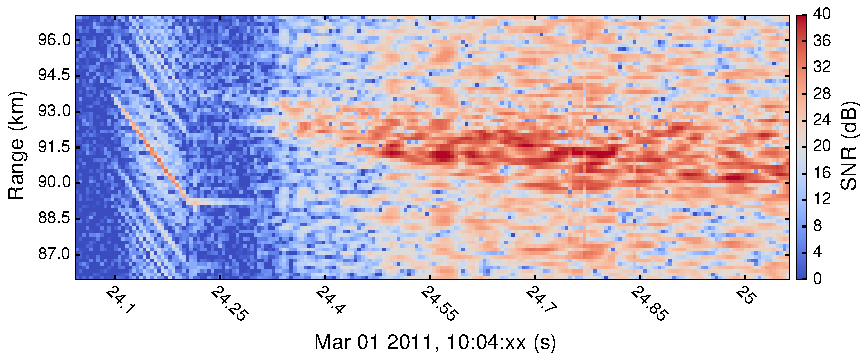
\includegraphics[trim=0px 20px 0px 3px,clip]{head_and_flare_mf_rti_4}
  \caption{Matched filter}
  \label{fig:example_mf_rti}
 \end{subfigure}
 
 \vspace{0.5\baselineskip}
 \begin{subfigure}{\textwidth}
  \centering
  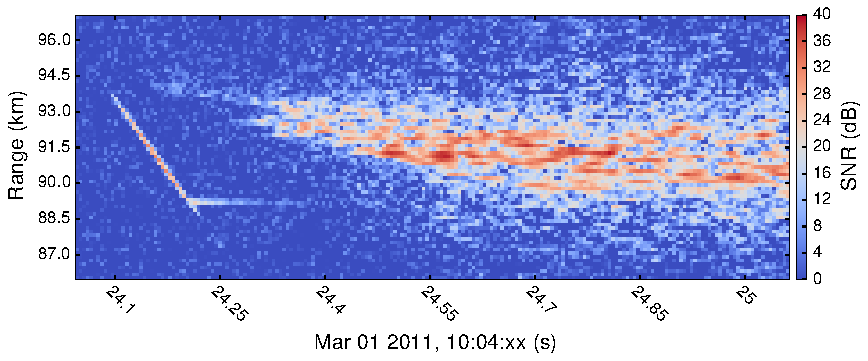
\includegraphics[trim=0px 20px 0px 3px,clip]{head_and_flare_recovered_rti_noise_4}
  \caption{Waveform inversion}
  \label{fig:example_recovered_rti}
 \end{subfigure}
 \caption[RTI comparison of matched filter and waveform inversion]{\emph{RTI comparison of matched filter and waveform inversion.} These images show the same pseudorandom-coded meteor head, flare, and trail from Figures \ref{fig:head_timeslice} and \ref{fig:trail_timeslice}. The matched filter result is for the peak-frequency-response of each pulse, while the waveform inversion result is the integrated power over all frequency coefficients. The elimination of delay-frequency sidelobes with waveform inversion reveals previously-obscured trail scattering and makes the true signal easier to identify.}
 \label{fig:mf_vs_recovered_rti}
\end{figure}%
The matched filter result in part (\subref{fig:example_mf_rti}) is for the peak-frequency-response filter for each individual pulse, selected from the entire frequency bank of 128 filters. The waveform inversion result in part (\subref{fig:example_recovered_rti}) is for the total signal summed across all frequency coefficients, which is sensible only because no delay-frequency sidelobes are present. The sparse solution's residual was matched filtered and added to the sparse coefficients to form the waveform inversion result as described in Section \ref{waveform_inversion_solution}.

As with the time slices of this data, waveform inversion is notable for removing the range sidelobes that clutter the matched filter result while retaining the high SNR of the true signal. There can be no doubt here that the waveform inversion method is beneficial. The pseudorandom code's autocorrelation function is clearly visible in the matched filter image, surrounding the descending head echo streak. With waveform inversion, those range sidelobes are completely eliminated to reveal previously-obscured trail scattering. Much of the clutter is also removed for the non-specular trail, although some artifacts remain. As previously discussed, these artifacts are likely the result of mismatch between the actual pulse waveform and its idealized representation in the radar model. Even with these artifacts, the result is much improved.

\subsection{Frequency Slices}
One way to minimize the effect of recovery mismatch artifacts is to analyze the individual frequency slices of the waveform inversion result. Frequency decomposition also makes it easy to separate and identify different types of signals. It is generally not possible to perform this type of analysis with a matched filter, since sidelobes of one target often obscure the features of another target even when separated in frequency. To demonstrate, Figure \ref{fig:recovered_dopplerslices} shows the first three positive frequency shifts, starting at zero, of the previous waveform inversion result.
\begin{figure}[tpb]
 \vspace{-1.5\baselineskip}
 \begin{subfigure}{\textwidth}
  \centering
  \textsf{\footnotesize Mar 01 2011, 10:04:xx (s)}
  
  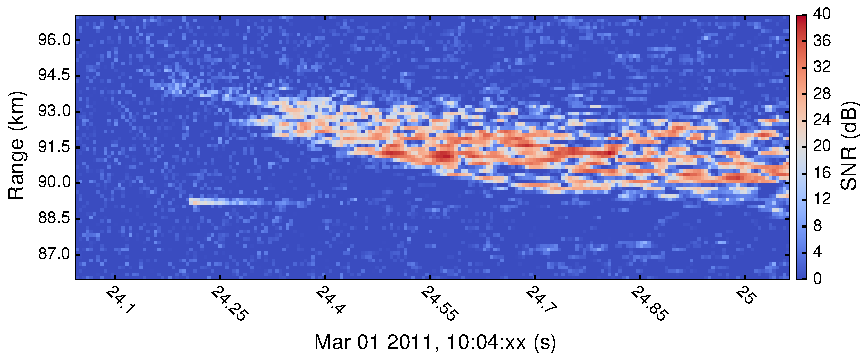
\includegraphics[trim=0px 20px 0px 3px,clip]{head_and_flare_recovered_doppler_rti_f0_p4}
  \caption{Zero frequency shift}
  \label{fig:recovered_dopplerslices_f0}
 \end{subfigure}
 
 \vspace{0.5\baselineskip}
 \begin{subfigure}{\textwidth}
  \centering
  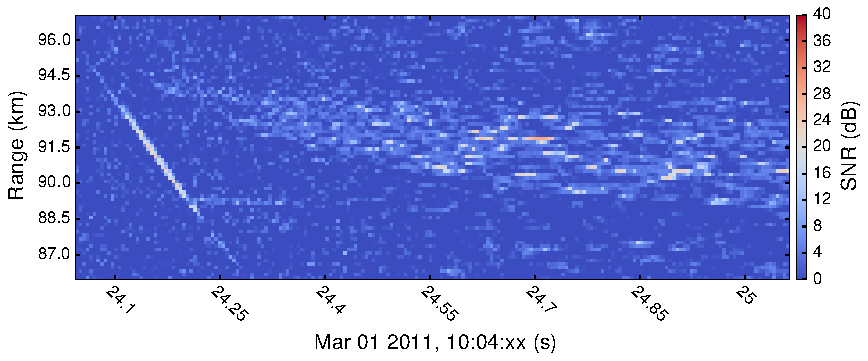
\includegraphics[trim=0px 20px 0px 3px,clip]{head_and_flare_recovered_doppler_rti_f1_p4}
  \caption{1st frequency step, 7.8 kHz shift ($-$23.4 km/s)}
  \label{fig:recovered_dopplerslices_f1}
 \end{subfigure}
 
 \vspace{0.5\baselineskip}
 \begin{subfigure}{\textwidth}
  \centering
  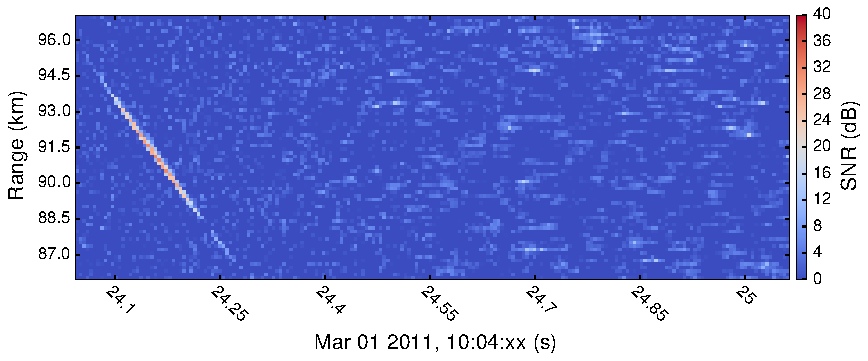
\includegraphics[trim=0px 20px 0px 3px,clip]{head_and_flare_recovered_doppler_rti_f2_p4}
  \caption{2nd frequency step, 15.6 kHz shift ($-$46.9 km/s)}
  \label{fig:recovered_dopplerslices_f2}
 \end{subfigure}
 \caption[Frequency slices of waveform inversion]{\emph{Frequency slices of waveform inversion.} These images show the same meteor head, flare, and trail from Figure \ref{fig:mf_vs_recovered_rti} decomposed over the first three frequency steps of the waveform inversion result. The stationary flare and trail appear in the zero-frequency slice, while the moving head echo appears at positive frequency shifts.}
 \label{fig:recovered_dopplerslices}
\end{figure}%

As nearly stationary targets, meteor trails exhibit only a small Doppler shift that is on the order of 100 m/s and is associated with the background neutral winds. Because this potential shift is very small compared to the waveform inversion frequency resolution, the flare and non-specular trail are clearly visible in the zero-frequency result. In contrast to the frequency-integrated RTI plot, the trail as shown at zero frequency is free from clear mismatch artifacts. The artifacts are spread randomly throughout the entire frequency space, so it is reasonable that they would not be very noticeable in any one frequency slice. The meteor head echo is visible in the image showing the first positive frequency shift, 7.8 kHz or $-$23.4 km/s in Doppler range rate. Although the true meteoroid velocity is higher, frequency spreading from discretization causes the signal to appear in this neighboring slice. A faint background of the trail is also visible in this image, along with a few points of higher SNR. The ghost trail is due to the frequency ambiguity of the code, and it appears as a result of applying the matched filter to the sparse solution's residual. This step is necessary to de-bias the sparse result and restore the signal that was shrunk toward zero. The second frequency step, 15.6 kHz or $-$46.9 km/s, is closest to the Doppler range rate of the head echo, and so its signal is strongest in the third plot. For the first time, we can also see that the head echo continues after disappearing for a few pulses; this is most likely due to the meteor exiting the main radar beam and reappearing in an antenna sidelobe. It is impossible to identify this feature in the matched filter or even the frequency-integrated result, but frequency decomposition allows us to find it. The absence of trail signal at the second frequency step is also reassuring, lending support to the theory that the signal seen in the first step is due to discretization spreading.

\subsection{Sparse Solution and Residual}
Next we investigate the separate sparse and measurement residual terms that form the waveform inversion result. The composition of the zero-frequency slice of the previous meteor example is shown in Figure \ref{fig:recovered_solution_composition}.
\begin{figure}[tpb]
 \vspace{-1.5\baselineskip}
 \begin{subfigure}{\textwidth}
  \centering
  \textsf{\footnotesize Mar 01 2011, 10:04:xx (s)}
  
  \includegraphics[trim=0px 20px 0px 3px,clip]{head_and_flare_recovered_doppler_rti_f0_p4}
  \caption{Waveform inversion combining sparse solution and residual}
  \label{fig:recovered_total}
 \end{subfigure}
 
 \vspace{0.5\baselineskip}
 \begin{subfigure}{\textwidth}
  \centering
  \includegraphics[trim=0px 20px 0px 3px,clip]{head_and_flare_recovered_sparse_doppler_rti_f0_p4}
  \caption{Sparse solution}
  \label{fig:recovered_sparse}
 \end{subfigure}
 
 \vspace{0.5\baselineskip}
 \begin{subfigure}{\textwidth}
  \centering
  \includegraphics[trim=0px 20px 0px 3px,clip]{head_and_flare_recovered_noise_doppler_rti_f0_p4}
  \caption{Matched filtered measurement residual}
  \label{fig:recovered_noise}
 \end{subfigure}
 \caption[Decomposition of waveform inversion as sparse and residual solutions]{\emph{Decomposition of waveform inversion as sparse and residual solutions.} The sparse solution is found by minimal $l_1$ fitting to the radar model, while the residual term is formed by matched filtering the remaining measurement error. Both contain important features that are added together to compose the waveform inversion solution.}
 \label{fig:recovered_solution_composition}
\end{figure}%
Figure \ref{fig:recovered_total} repeats the complete waveform inversion image, while Figures \ref{fig:recovered_sparse} and \ref{fig:recovered_noise} show the sparse and residual components.

As expected, the sparse solution contains all of the significant coefficients that represent the flare and trail scattering. It is truly sparse, with most of the shown zero-frequency coefficients and the vast majority of the unshown nonzero-frequency coefficients equal to zero. The sparse solution is excellent for identifying targets and examining the high-SNR components, but it does not provide all of the needed information. Since the sparse solution by itself is biased toward zero, the residual contains not only noise but also remaining elements of the signal that fall below the detection threshold. The additional signal that is necessary to de-bias the sparse solution is clearly visible for the flare and trail. This low-SNR element also includes crucial details like the initial formation of the trail and the continuation of the flare. Since it is matched filtered, the residual also contains sidelobes for that signal, but the sidelobes are necessarily so far below the noise level that they are inconsequential. When combined together into the waveform inversion result, all of the relevant features of the signal are visible for easy comparison and analysis. Nevertheless, it is still important to remember how those elements were formed.

\subsection{Detection Sensitivity}
In Figure \ref{fig:longtrail_recovery_rti_comparison}, we show RTI images for a different meteor in order to lend more support to our waveform inversion observations.
\begin{figure}[tpb]
 \vspace{-1.5\baselineskip}
 \begin{subfigure}{\textwidth}
  \centering
  \textsf{\footnotesize Mar 01 2011, 10:09:xx (s)}
  
  \includegraphics[trim=0px 20px 0px 3px,clip]{longtrail_mf_rti_4}
  \caption{Matched filter}
  \label{fig:longtrail_mf_rti}
 \end{subfigure}
 
 \vspace{0.5\baselineskip}
 \begin{subfigure}{\textwidth}
  \centering
  \includegraphics[trim=0px 20px 0px 3px,clip]{longtrail_recovered_rti_noise_4}
  \caption{Waveform inversion}
  \label{fig:longtrail_recovered_rti}
 \end{subfigure}
 
 \vspace{0.5\baselineskip}
 \begin{subfigure}{\textwidth}
  \centering
  \includegraphics[trim=0px 20px 0px 3px,clip]{longtrail_mf_rti_3}
  \caption{Matched filter for LFM chirp}
  \label{fig:longtrail_mf_lfm_rti}
 \end{subfigure}
 \caption[Waveform inversion example for a different meteor]{\emph{Waveform inversion example for a different meteor.} The method is successful even with head echo and non-specular trail signals overlapping in the same pulse. This comparison includes the matched filter result for the neighboring LFM chirp pulses, which does a better job of differentiating the head echo.}
 \label{fig:longtrail_recovery_rti_comparison}
\end{figure}%
The matched filter result for the pseudorandom code is shown, followed by the corresponding waveform inversion result. A third image showing the matched filter result for the LFM chirp is also given in order to compare detection of the entire head echo. The overall conclusion taken from this data is the same as that from the previous example: waveform inversion is very successful at eliminating sidelobes and making obscured features visible, but it can also include artifacts from waveform mismatch. Comparison with the LFM chirp, which features the best matched filter results due to its unique delay-frequency ambiguity, reveals something new: signals with lower SNR are not always recoverable with a given waveform. The head echo is longer and better-defined with the LFM chirp. Waveform inversion makes more of the head echo evident than what is visible with the comparable matched filter, but we have clear evidence that it is possible to do better. The loss of signal on the head echo could just be due to actual- and ideal-code mismatch, but it is at least something to note for analyzing other results. Overall, waveform inversion with the pseudorandom code gives results that are clearly superior to the LFM chirp.

\section{Waveform Comparison Results}
In this section we compare the inversion performance of the various waveforms used in the Jicamarca experiment. Our results show that the success of the technique depends primarily upon the waveform's ambiguity function, but the quality of the recovery is more sensitive to pulse length and the fidelity of the transmitted waveform to its idealized representation.

\subsection{Minimum Peak Sidelobe Code}
The minimum peak sidelobe code enables waveform inversion with as much success as the pseudorandom code. Their identical length means that they should be able to recover signals with the same sensitivity, but it is reassuring to know that the minimum sidelobe code is suitably incoherent. The original meteor example returns in Figure \ref{fig:msl_comparison} with a comparison between the matched filter, frequency-integrated waveform inversion, and zero-frequency waveform inversion results.
\begin{figure}[tpb]
 \vspace{-1.5\baselineskip}
 \begin{subfigure}{\textwidth}
  \centering
  \textsf{\footnotesize Mar 01 2011, 10:04:xx (s)}
  
  \includegraphics[trim=0px 20px 0px 3px,clip]{head_and_flare_mf_rti_1}
  \caption{Matched filter}
  \label{fig:msl_mf}
 \end{subfigure}
 
 \vspace{0.5\baselineskip}
 \begin{subfigure}{\textwidth}
  \centering
  \includegraphics[trim=0px 20px 0px 3px,clip]{head_and_flare_recovered_rti_noise_1}
  \caption{Frequency-integrated waveform inversion}
  \label{fig:msl_recovered}
 \end{subfigure}
 
 \vspace{0.5\baselineskip}
 \begin{subfigure}{\textwidth}
  \centering
  \includegraphics[trim=0px 20px 0px 3px,clip]{head_and_flare_recovered_doppler_rti_f0_p1}
  \caption{Zero-frequency slice of waveform inversion}
  \label{fig:msl_recovered_dopplerslice}
 \end{subfigure}
 \caption[Waveform inversion with the minimum peak sidelobe code]{\emph{Waveform inversion with the minimum peak sidelobe code.} With its good sidelobe properties, the minimum sidelobe code also demonstrates successful waveform inversion. Sidelobes are eliminated to provided a cleaner image, although the frequency-integrated result still suffers from mismatch artifacts.}
 \label{fig:msl_comparison}
\end{figure}%
Aside from a little leakage of the head echo into the zero-frequency result, the minimum sidelobe results exhibit the same features as the pseudorandom results. Given the better range sidelobe properties of the optimal minimum sidelobe code, one might hope that it might somehow be able to do better than pseudorandom code. While this may still be the case for scenes that push the sparsity limit, the difference between the codes is inconsequential in this case. This fact is not entirely surprising either, since the complete set of delay-frequency sidelobes for the minimum sidelobe code are not necessarily any more suitable for waveform inversion than those of the pseudorandom code.

\subsection{Barker-13 Code}
The Barker-13 code also has good sidelobe properties, so we would expect it to find success as well. Given its shorter length, however, it is less sensitive and more likely to have signals lost in the noise. Figure \ref{fig:b13_comparison} provides the now-familiar comparison images between matched filtering and waveform inversion.
\begin{figure}[tpb]
 \vspace{-1.5\baselineskip}
 \begin{subfigure}{\textwidth}
  \centering
  \textsf{\footnotesize Mar 01 2011, 10:04:xx (s)}
  
  \includegraphics[trim=0px 20px 0px 3px,clip]{head_and_flare_mf_rti_0}
  \caption{Matched filter}
  \label{fig:b13_mf}
 \end{subfigure}
 
 \vspace{0.5\baselineskip}
 \begin{subfigure}{\textwidth}
  \centering
  \includegraphics[trim=0px 20px 0px 3px,clip]{head_and_flare_recovered_rti_noise_0}
  \caption{Frequency-integrated waveform inversion}
  \label{fig:b13_recovered}
 \end{subfigure}
 
 \vspace{0.5\baselineskip}
 \begin{subfigure}{\textwidth}
  \centering
  \includegraphics[trim=0px 20px 0px 3px,clip]{head_and_flare_recovered_doppler_rti_f2_p0}
  \caption{2nd frequency shift of waveform inversion, 15.6 kHz ($-$46.9 km/s)}
  \label{fig:b13_recovered_dopplerslice}
 \end{subfigure}
 \caption[Waveform inversion with the Barker-13 code]{\emph{Waveform inversion with the Barker-13 code.} The technique is moderately successful with the Barker-13 code. It effectively eliminates sidelobes, but as a result of the pulse's short length, a ghost trail from the zero-frequency matched filtered residual spreads into the 2nd frequency step.}
 \label{fig:b13_comparison}
\end{figure}%
Since the observed meteor has a high SNR, waveform inversion is successful with the Barker-13 code in this case. The example also shows the slice for the second frequency shift of the waveform inversion solution. This plot best demonstrates the effects of another downside of a shorter pulse: wider frequency spread in the matched filter ambiguity function. Because the matched filter is applied to the sparse solution's residual, the wider frequency spread results in the zero-frequency residual ghost trail being visible two frequency steps away. If shorter pulses must be used, the Barker-13 code is still a suitable one for waveform inversion. However, given the benefits of using a longer code and the success we have demonstrated in eliminating sidelobes, there no longer seems to be a reason to restrict oneself to shorter codes when the necessary computing resources are available to do better.

\subsection{Uncoded Pulse}
The uncoded pulse has a terrible ambiguity function, and we might expect that it would be correspondingly ill-suited to waveform inversion. This is not the case, as shown in Figure \ref{fig:unc_comparison}.
\begin{figure}[tpb]
 \vspace{-1.5\baselineskip}
 \begin{subfigure}{\textwidth}
  \centering
  \textsf{\footnotesize Mar 01 2011, 10:04:xx (s)}
  
  \includegraphics[trim=0px 20px 0px 3px,clip]{head_and_flare_mf_rti_2}
  \caption{Matched filter}
  \label{fig:unc_mf}
 \end{subfigure}
 
 \vspace{0.5\baselineskip}
 \begin{subfigure}{\textwidth}
  \centering
  \includegraphics[trim=0px 20px 0px 3px,clip]{head_and_flare_recovered_rti_noise_2}
  \caption{Frequency-integrated waveform inversion}
  \label{fig:unc_recovered}
 \end{subfigure}
 
 \vspace{0.5\baselineskip}
 \begin{subfigure}{\textwidth}
  \centering
  \includegraphics[trim=0px 20px 0px 3px,clip]{head_and_flare_recovered_doppler_rti_f0_p2}
  \caption{Zero-frequency slice of waveform inversion}
  \label{fig:unc_recovered_dopplerslice}
 \end{subfigure}
 \caption[Waveform inversion with the uncoded pulse]{\emph{Waveform inversion with the uncoded pulse.} Despite sidelobes that completely obscure the matched filter result, waveform inversion is successful at recovering the meteor scatter. Mismatch artifacts are also minimized in comparison to the coded pulses, producing a cleaner frequency-integrated result.}
 \label{fig:unc_comparison}
\end{figure}%
Waveform inversion successfully eliminates the sidelobes of the uncoded pulse and recovers a solution that is similar to the other waveforms. There are both negatives and positives with the uncoded pulse. On the one hand, the zero-frequency result shows that it misses some of the lower-SNR details that the other waveforms reveal in the meteor trail, and the matched filtered residual still produces prominent ghost sidelobes. On the other hand, the mismatch between the ideal waveform and its idealized model is reduced for the uncoded pulse without the complexities of coding, and the frequency-integrated result is relatively free of artifacts. It is still expected that an uncoded pulse will produce measurements that are more coherent than most codes, causing the waveform inversion to struggle in recovering denser solutions. However, the uncoded pulse has taught us that the more important consideration is waveform fidelity. Therefore, uncoded or lower-bandwidth pulses may be used if needed to ensure fidelity.

\subsection{LFM Chirp}
The LFM chirp has a very special ambiguity function; it is compact along a line in delay-frequency space, but within that line it is extremely ambiguous. As it turns out, that ambiguity is too much to overcome, and the LFM chirp is the only waveform that we tested that completely fails waveform inversion. The evidence is given in Figure \ref{fig:lfm_comparison}.
\begin{figure}[tpb]
 \vspace{-1.5\baselineskip}
 \begin{subfigure}{\textwidth}
  \centering
  \textsf{\footnotesize Mar 01 2011, 10:04:xx (s)}
  
  \includegraphics[trim=0px 20px 0px 3px,clip]{head_and_flare_mf_rti_3}
  \caption{Matched filter}
  \label{fig:lfm_mf}
 \end{subfigure}
 
 \vspace{0.5\baselineskip}
 \begin{subfigure}{\textwidth}
  \centering
  \includegraphics[trim=0px 20px 0px 3px,clip]{head_and_flare_recovered_rti_noise_3}
  \caption{Waveform inversion}
  \label{fig:lfm_recovered}
 \end{subfigure}
 \caption[Waveform inversion with the LFM chirp]{\emph{Waveform inversion with the LFM chirp.} The ridge of delay-frequency ambiguity, a defining property of the LFM chirp, makes waveform inversion impossible. The head echo gains more sidelobes but is still visible, while the trail scattering is represented by completely non-physical reflectivities.}
 \label{fig:lfm_comparison}
\end{figure}%
Without a clear delay-frequency peak produced by the matched filter bank, the sparse approximation algorithm can't pinpoint scatterers, and recovery is impossible. In the parlance of compressed sensing, the measurements are too coherent in the delay-frequency dictionary to allow for undersampling. To make matters worse, it must be noted that the radar model doesn't really accommodate the LFM chirp since it requires a discrete code with constant bauds. To perform waveform inversion (or apply digital matched filtering), the continuous frequency sweep has to be discretized. These problems should not be read as an indictment of all chirp waveforms, however. Truly discrete chirps require no special treatment, and the ridge ambiguity is only a property of the linear chirp. Judging from the ambiguity function, we expect that a quadratic or other type of chirp (e.g. an Alltop sequence) would have properties sufficient for inversion.

\subsection{Inter-waveform Comparison}
The relative performance of each of the waveforms can already be inferred by comparing the plots of each of their results, but displaying them together will make the comparison easier. We return to the second meteor example and present the waveform inversion results for the pseudorandom code, minimum sidelobe code, and uncoded pulse. These are shown in Figure \ref{fig:waveform_comparison} as frequency-integrated RTI plots and in Figure \ref{fig:waveform_comparison_doppler0} as zero-frequency slices.
\begin{figure}[tpb]
 \vspace{-1.5\baselineskip}
 \begin{subfigure}{\textwidth}
  \centering
  \textsf{\footnotesize Mar 01 2011, 10:09:xx (s)}
  
  \includegraphics[trim=0px 20px 0px 3px,clip]{longtrail_recovered_rti_noise_4}
  \caption{Pseudorandom code, PSRND$_\text{51}$}
  \label{fig:longtrail_psrnd_recovered}
 \end{subfigure}
 
 \vspace{0.5\baselineskip}
 \begin{subfigure}{\textwidth}
  \centering
  \includegraphics[trim=0px 20px 0px 3px,clip]{longtrail_recovered_rti_noise_1}
  \caption{Minimum peak sidelobe code, MSL$_\text{51}$}
  \label{fig:longtrail_msl_recovered}
 \end{subfigure}
 
 \vspace{0.5\baselineskip}
 \begin{subfigure}{\textwidth}
  \centering
  \includegraphics[trim=0px 20px 0px 3px,clip]{longtrail_recovered_rti_noise_2}
  \caption{Uncoded pulse}
  \label{fig:longtrail_unc_recovered}
 \end{subfigure}
 \caption[Frequency-integrated waveform inversions of different waveforms]{\emph{Frequency-integrated waveform inversions of different waveforms.} These images compare results for the second meteor example. They reveal that the significant signals are common to all of the waveforms, but the lower-SNR artifacts differ. This is evidence that the artifacts are related to transmitted waveform mismatch.}
 \label{fig:waveform_comparison}
\end{figure}%
\begin{figure}[tpb]
 \vspace{-1.5\baselineskip}
 \begin{subfigure}{\textwidth}
  \centering
  \textsf{\footnotesize Mar 01 2011, 10:09:xx (s)}
  
  \includegraphics[trim=0px 20px 0px 3px,clip]{longtrail_recovered_doppler_rti_f0_p4}
  \caption{Pseudorandom code, PSRND$_\text{51}$}
  \label{fig:longtrail_psrnd_doppler0}
 \end{subfigure}
 
 \vspace{0.5\baselineskip}
 \begin{subfigure}{\textwidth}
  \centering
  \includegraphics[trim=0px 20px 0px 3px,clip]{longtrail_recovered_doppler_rti_f0_p1}
  \caption{Minimum peak sidelobe code, MSL$_\text{51}$}
  \label{fig:longtrail_msl_doppler0}
 \end{subfigure}
 
 \vspace{0.5\baselineskip}
 \begin{subfigure}{\textwidth}
  \centering
  \includegraphics[trim=0px 20px 0px 3px,clip]{longtrail_recovered_doppler_rti_f0_p2}
  \caption{Uncoded pulse}
  \label{fig:longtrail_unc_doppler0}
 \end{subfigure}
 \caption[Zero-frequency waveform inversion slices of different waveforms]{\emph{Zero-frequency waveform inversion slices of different waveforms.} The coded pulses produce remarkably similar results when mismatch artifacts are not considered, while the uncoded pulse lags behind somewhat. The consistency is evidence that the results are close to the true sparse solution.}
 \label{fig:waveform_comparison_doppler0}
\end{figure}%
The comparison of these results is our basis for claiming that the artifacts present in the solution, and most noticeable in the frequency-integrated plots, are based on waveform mismatch. Each of the waveforms produces an image that agrees for the location and strength of the significant scattering. Sensitivity to low SNR scattering is more variable, but by examining the frequency slices it becomes clear which of the lower-SNR signals are true scattering and which are artifacts spread across all frequency steps. Since the form of these artifacts changes with each of the codes, they are a code-dependent property. Since the artifacts are minimized with the uncoded pulse, we conclude that they are a result of mismatch between the actual waveform and its idealized model.

The zero-frequency slices are more illuminating when it comes to revealing the recovery properties of the waveforms themselves and not that of these particular imperfect measurements. The slices clearly show that the coded pulses are strictly better than the uncoded pulse in accurately recovering the meteor trail. Significant features present in the coded pulse results are absent with the uncoded pulse, and it seems more likely that it is a failing of the latter rather than a coincidence of the former. Stripping away most of the waveform artifacts, as with these zero-frequency inversion results for the coded pulses, gives the clearest image of trail scattering that we can produce. Their degree of similarity is amazing, and it must be representative of the fact that we are getting close to the true solution.

\section{Undersampling Results}
One unexplored property of the waveform inversion method is the ability to set the model undersampling factor $R$ to a value greater than 1, which would achieve higher resolution results. The method has proven useful for sidelobe elimination, but sparsity could allow us to accomplish more by truly taking advantage of the compression aspect of compressed sensing. Theoretically, the key to recovery at increased resolution is still measurement incoherence, and the best way to likely ensure that is to increase the bandwidth of the transmitted waveform. As we have seen with the uncoded pulse, however, that is not a necessary condition for success.

\subsection{Discarding Half the Data}
In lieu of being able to validate the increased resolution with $R>1$ using the matched filter, as we have done with the previous results, we can deliberately undersample the existing data and use our full knowledge as a basis of comparison. In Figure \ref{fig:half_sampling_comparison}, we compare waveform inversion with half of the data samples (keeping every other one) to waveform inversion with the full data set.
\begin{figure}[tpb]
 \vspace{-1.5\baselineskip}
 \begin{subfigure}{\textwidth}
  \centering
  \textsf{\footnotesize Mar 01 2011, 10:04:xx (s)}
  
  \includegraphics[trim=0px 20px 0px 3px,clip]{head_and_flare_half_recovered_rti_noise_4}
  \caption{Half the samples, frequency-integrated}
  \label{fig:half_recovered}
 \end{subfigure}
 
 \vspace{0.5\baselineskip}
 \begin{subfigure}{\textwidth}
  \centering
  \includegraphics[trim=0px 20px 0px 3px,clip]{head_and_flare_half_recovered_doppler_rti_f0_p4}
  \caption{Half the samples, zero-frequency slice}
  \label{fig:half_recovered_doppler0}
 \end{subfigure}
 
 \vspace{0.5\baselineskip}
 \begin{subfigure}{\textwidth}
  \centering
  \includegraphics[trim=0px 20px 0px 3px,clip]{head_and_flare_recovered_doppler_rti_f0_p4}
  \caption{All samples, zero-frequency slice}
  \label{fig:recovered_doppler0}
 \end{subfigure}
 \caption[Waveform inversion with half the data]{\emph{Waveform inversion with half the data.} Waveform inversion was performed after discarding half of the pseudorandom pulse samples, and the results are compared to fully-sampled inversion. Head echo recovery is congruent with the previous results, but the trail is too sparse, indicating that the undersampling is too severe.}
 \label{fig:half_sampling_comparison}
\end{figure}%
Since the best waveform inversion results have been the single-frequency slices with the pseudorandom pulse, that is what we have compared between the half-sampled and fully-sampled data. Though the frequency-integrated image is rife with mismatch artifacts, overall they are not much worse than what was frequently encountered with the fully-sampled data. The zero-frequency slice tells the full story, though, and the results are mixed. With half the samples, we expect the result to have half the SNR, but much more of the signal is missing. The features with the highest SNR are still present for the most part, but the surrounding scattering with lower SNR is eliminated with half the data. However, the head echo is still recovered quite well, matching our expectations from the full data set exactly. It seems most likely that half the data is not enough to recover a signal with the number of nonzero coefficients required by the trail. Instead of the full solution, what we get is the closest sparse approximation with the maximum number of coefficients that can be recovered with the given number of measurements.

\subsection{Recovering at Double Resolution}
Even with mixed success at recovering consistent results from half-sampled data, we proceed to attempt recovery at double the resolution of the fully-sampled data. At a minimum, we hope that the head echo resolution can be increased successfully. The transmitted waveforms were sampled at their bandwidth, so doubling the model sampling rate nominally makes the waveforms ambiguous over the width of two samples. This is not necessarily an insurmountable problem, as recovery with the fully ambiguous uncoded pulse shows. A consistent theme has been that the actual waveforms don't exactly match the idealized waveforms, and in reality they do vary within the "constant" bauds of each code. To perform this double-resolution recovery, we have attempted to use the non-ideality to our advantage. Rather than doubling the length of the ideal codes by repeating each of the bauds, we simulated the effects of the transmitter's limited bandwidth by upsampling and lowpass filtering the ideal codes. The result is a double-resolution waveform that should vary in a manner similar to the actual waveform.

Figure \ref{fig:increased_resolution_comparison} shows the double-resolution recovery results for the first meteor example using the pseudorandom waveform data and the upsampled, lowpass-filtered pseudorandom code. Figure \ref{fig:longtrail_increased_resolution} shows the same for the second meteor example.
\begin{figure}[tpb]
 \vspace{-1.5\baselineskip}
 \begin{subfigure}{\textwidth}
  \centering
  \textsf{\footnotesize Mar 01 2011, 10:04:xx (s)}
  
  \includegraphics[trim=0px 20px 0px 3px,clip]{head_and_flare_lowpass_up_recovered_rti_noise_4}
  \caption{Double resolution, frequency-integrated}
  \label{fig:lowpass_up_recovered}
 \end{subfigure}
 
 \vspace{0.5\baselineskip}
 \begin{subfigure}{\textwidth}
  \centering
  \includegraphics[trim=0px 20px 0px 3px,clip]{head_and_flare_lowpass_up_recovered_doppler_rti_f0_p4}
  \caption{Double resolution, zero-frequency slice}
  \label{fig:lowpass_up_recovered_doppler0}
 \end{subfigure}
 
 \vspace{0.5\baselineskip}
 \begin{subfigure}{\textwidth}
  \centering
  \includegraphics[trim=0px 20px 0px 3px,clip]{head_and_flare_recovered_doppler_rti_f0_p4}
  \caption{Normal resolution, zero-frequency slice}
  \label{fig:recovered_doppler0_again}
 \end{subfigure}
 \caption[Waveform inversion at double the resolution]{\emph{Waveform inversion at double the resolution.} To recover a double-resolution solution for the first meteor example, we upsampled and lowpass-filtered the pseudorandom code to simulate the effects of the actual transmitter's limited bandwidth. The results are promising, with all features represented consistently.}
 \label{fig:increased_resolution_comparison}
\end{figure}%
\begin{figure}[tpb]
 \vspace{-1.5\baselineskip}
 \begin{subfigure}{\textwidth}
  \centering
  \textsf{\footnotesize Mar 01 2011, 10:09:xx (s)}
  
  \includegraphics[trim=0px 20px 0px 3px,clip]{longtrail_lowpass_up_recovered_doppler_rti_f0_p4}
  \caption{Double resolution, frequency-integrated}
  \label{fig:psrnd_lowpass_up_doppler0}
 \end{subfigure}
 
 \vspace{0.5\baselineskip}
 \begin{subfigure}{\textwidth}
  \centering
  \includegraphics[trim=0px 20px 0px 3px,clip]{longtrail_lowpass_up_recovered_doppler_rti_f0_p1}
  \caption{Double resolution, zero-frequency slice}
  \label{fig:msl_lowpass_up_doppler0}
 \end{subfigure}
 
 \vspace{0.5\baselineskip}
 \begin{subfigure}{\textwidth}
  \centering
  \includegraphics[trim=0px 20px 0px 3px,clip]{longtrail_recovered_doppler_rti_f0_p4}
  \caption{Normal resolution, zero-frequency slice}
  \label{fig:psrnd_doppler0}
 \end{subfigure}
 \caption[Waveform inversion at double the resolution, second example]{\emph{Waveform inversion at double the resolution, second example.} Doubling the resolution of the second meteor example also produces promising results. One can easily imagine that the normal-resolution image is a blurred version of the double-resolution image. However, it is impossible to determine whether that is truly the case.}
 \label{fig:longtrail_increased_resolution}
\end{figure}%
Whether the difference is a better relative sparsity or the fact that the lowpass-filtered code better represents the true waveform, these double resolution results \emph{look} better than the half-sampled results. In both examples, the mismatch artifacts appear to be noticeably reduced in the frequency-integrated image, and the double-resolution image has all of the same significant features as the normal-resolution image. In fact, it is easy to imagine that the original results represent a blurred version of the "true" increased-resolution results. Do the localized striations of the double-resolution trails give a better representation of the plasma and scattering physics? Without further support and given the half-sampled recovery results, it is impossible to declare victory and claim that we have successfully doubled the range resolution of our measurements. Regardless, the method looks promising and definitely merits further research.

\section{Recommendations}
\subsection{Waveform Selection}
The waveform inversion results have demonstrated the method's usefulness, eliminating sidelobes in these examples and in our additional informal testing. It works with a variety of codes, even with uncoded pulses, but the best results were achieved with the longest codes. It is impossible to replace the sensitivity provided by a long code, and with the effect of sidelobes minimized, there is no reason to not use the longest possible pulse length. The other consideration is the code itself, and on that point we have less evidence. Removing pulse length and the clearly-suboptimal uncoded and LFM chirp ambiguities from the equation, the remaining three codes seemed to find similar success. Based on our knowledge of the solution procedure as iterative matched filtering and thresholding steps, we can make the educated guess that codes with lower peak sidelobes across the entire delay-frequency space will perform better. There is obviously less work for the recovery algorithm to do when the matched filter already does a good job. Overall, the recommendation is to use long codes with minimal delay-frequency sidelobes, which are not necessarily the minimum peak range sidelobe codes.

The other waveform consideration is fidelity with the actual transmission. The most significant artifacts in the inversion result are likely an effect of mismatch between the transmitted waveform and its idealized representation in the model. The relative success of the uncoded pulse, at least with respect to artifacts, points to this conclusion. Codes should be selected knowing the bandwidth constraints and performance characteristics of the transmitter in order to ensure that the outgoing waveform is as desired. There will always be non-idealities, however, so it is recommended that one take the additional step of sampling the transmitted waveform. With transmitter samples, it is possible to use code values that most closely match the actual waveform, and thus mismatch artifacts should be minimized.

\subsection{Frequency Analysis}
Another problem we encountered is the poor frequency resolution that results from using a relatively low-frequency radar like Jicamarca. Future work could involve developing a multi-pulse inversion method, or alternatively, use a radar that operates at a higher frequency. Another possibility for increasing frequency resolution is to increase the number of frequency steps $N$ included in the radar model. Doing so can help to improve relative sparsity as discussed in Section \ref{point_target_reflectivity}, but there are limits. Larger $N$ means more unknown variables, which means proportionally longer calculations. Larger $N$ also means making the measurements more coherent in terms of the solution space, so there is a point at which increasing $N$ would result in the failure to find the true solution. For these reasons, we recommend setting $N$ as low as possible to achieve the desired frequency resolution, optimally to the minimum value of the length $L$ of the waveform code. When this is done with sufficiently long codes, the true solution is likely to still be sparse enough to permit recovery.

The ability to decompose the waveform inversion solution into different frequency slices is a real strength of the analysis method. Though a frequency-integrated plot gives a good overview of the recovered scene, the individual frequency slices can be used to identify particular targets and better-observe their details. Even when targets that scatter at different frequency shifts are present at the same ranges, waveform inversion can separate them for individual analysis. This ability is most useful for crowded radar scenes like those encountered in the equatorial ionosphere at Jicamarca. Making full use of this capability when designing waveform inversion experiments is highly recommended.

\subsection{Computation}
One final difficulty with the waveform inversion method is the time it takes to compute the recovery solution. Instead of applying the matched filter once per pulse, inversion requires, at minimum, applying it and the forward model on the order of a hundred times. Even with an efficient implementation and quick convergence, that takes a significant amount of time. Fortunately, the method as it stands now is eminently parallelizable; each pulse is processed individually, and there is no reason that they cannot be processed at the same time instead of in sequence. For larger applications, this would certainly be recommended.

\part{Conclusion}
\label{part_conclusion}
\chapter{Conclusion}
\label{conclusion}
With the goal of enabling flexible, high-resolution measurements of ionospheric plasma phenomena, this thesis draws upon the subjects of radar analysis, sparse approximation, and convex optimization to develop and apply a novel waveform inversion method. In Part \ref{part_introduction}, we introduced these subjects and described the challenges encountered with ionospheric radar measurements that arise from the inherent conflict between sensitivity and ambiguity. Current techniques struggle to meet the following goals:
\begin{inparaenum}[1)]
 \item Differentiation of targets in crowded and variable environments, which is necessary to separate meteor and electrojet signals in the equatorial ionosphere;
 \item Elimination of self-interference of range- or frequency-spread targets, including non-specular meteor trails;
 \item High range and frequency resolution for observing small-scale processes, such as meteoroid fragmentation and meteor flares; and
 \item Flexibility to achieve these goals for a variety of waveform and measurement requirements arising from experimental and hardware constraints.
\end{inparaenum}
Waveform inversion can achieve these goals. In Part \ref{part_radar_analysis}, we reviewed the traditional radar matched filtering technique and the ambiguity that it introduces, and we proposed a mathematical model to describe radar measurements in terms of ambiguity-free reflectivity coefficients. In Part \ref{part_waveform_inversion}, we addressed the complete problem of waveform inversion, from the theory of compressed sensing via convex optimization to the implementation of efficient algorithms and the application to actual radar data. In this chapter, we conclude with a discussion of contributions and a sketch of potential further research.

\section{Summary and Discussion of Contributions}
\label{discussion}
\subsection{Radar Model}
\begin{italicquote}
A new perspective for radar measurements is espoused in which the radar scene reflectivity is recovered by inverting a mathematical model.
\end{italicquote}

Radar measurements in their basic form, a sequence of values sampled from the received signal, are not amenable to information processing when pulses longer than the sampling period are used. Our radar model addresses this by representing the measurements as a function of delay-frequency reflectivity coefficients. The use of a delay-frequency dictionary is useful because the coefficients are typically sparse. A similar delay-frequency analysis is also possible with a bank of frequency-shifted matched filters, but that representation is blurred with respect to the true reflectivities due to waveform ambiguity. We first introduced the radar model in Chapter \ref{radar_model} with exactly this imaging analogy; the ambiguity function acts as a point-spread function when matched filtering is applied to the measurements, blurring the true radar scene's reflectivity. The forward radar model is the adjoint of the matched filter bank operation, and as a consequence, matched filtering gives the least-norm solution to the radar model measurement equation. Instead, knowing that a sparse solution is most likely to be correct, we posed the following waveform inversion problem: invert the radar model with sparsity as a constraint to recover the sidelobe-free radar scene.

\begin{italicquote}
 A discrete radar model is rigorously derived from the continuous measurement equation for a general target scene.
\end{italicquote}

We followed the informal radar model presentation with a rigorous derivation to determine precisely how general radar scenes are represented. Starting from the continuous narrow-band radar measurement equation, the discrete radar model was re-derived through discretization and Fourier analysis. Notably, this derivation only assumes what is typical for matched filter analysis: a narrow-band signal, no scattering from outside the delay window of interest, uniform sampling of the received signal, a transmission waveform represented by a code sequence describing constant bauds, and a number of frequency steps greater than the length of the code. The resulting radar model is discrete, with a fixed number of reflectivity coefficients corresponding to a delay-frequency grid. Point targets falling on the grid points are naturally represented, but off-grid point targets and distributed targets are also accommodated. The derivation shows that arbitrary targets are written exactly, though not uniquely, in terms of the gridded coefficients. With respect to delay, the coefficients represent the integrated reflectivity over the corresponding delay window; with respect to frequency, the coefficients represent samples from the complete reflectivity function after it has been convolved with a periodic sinc function. Because of this known relationship, we can infer that sparsity of the full radar scene, as represented by the continuous reflectivity function, is reasonably preserved as sparsity of the discrete reflectivity coefficients. Thus, the waveform inversion procedure is justified.

\subsection{Waveform Inversion Method}
\begin{italicquote}
 A novel waveform inversion technique is formulated based on finding a sparse representation of the radar scene using the discrete model.
\end{italicquote}

Sparse solutions to underdetermined systems of equations is the domain of the theory of compressed sensing, which states that minimizing the $l_1$-norm when constrained by enough incoherent measurements guarantees recovery of the true sparse solution. In Chapter \ref{waveform_inversion}, a review of theoretical results indicated that recovery of the reflectivity coefficients using the radar model is likely to be successful provided that a suitable waveform is used. All that is required are global, incoherent measurements, which are ensured by random binary-phase sequences, the Alltop quadratic chirp sequences, and likely many more waveforms. With successful recovery, waveform inversion meets all of the goals that existing methods fail to reach. Elimination of delay-frequency sidelobes, and their ambiguity, is inherent to the method. That, coupled with the simultaneous decoding over the signal's full frequency spectrum provided by waveform inversion, enables target differentiation for multiple or distributed scatterers in crowded and variable environments. Given a sufficient level of sparsity, inversion can also provide solutions with a higher resolution than that specified by the sampling rate, thus enabling better observations of small-scale processes. Since recovery is likely with many different waveforms, the method is also flexible enough to be used when there is little or no freedom in choosing the waveform or dictating the experimental setup.

In practical terms, the waveform inversion solution procedure is straightforward. Our approach, detailed in Chapter \ref{waveform_inversion}, is to solve an $l_1$-regularized least squares problem using a first-order convex optimization method that involves the soft-thresholding proximal operator. Algorithms like this have an intuitive interpretation in radar terms as an iterative thresholding matched filter: each step involves applying the matched filter to detect under-represented components and thresholding the new representation to induce sparsity. The optimization problem's regularization parameter $\lambda$ is chosen to ensure a constant false-alarm rate for detection based on an independently-estimated noise level. In order to compare the inversion to matched filtering and de-bias the result, the solution is scaled and added to its matched filtered measurement residual. Adding the residual term also has the benefit of including any signal that falls below the detection threshold. As a result, the regularization parameter (detection threshold) serves as the threshold for sidelobe elimination: sidelobes are removed for signals with magnitude above the threshold and left intact for signals with magnitude below the threshold. Larger thresholds result in faster convergence, so there is a direct trade-off between speed and sidelobe elimination.

\begin{italicquote}
 The waveform inversion method is implemented using modern convex optimization techniques tailored for efficient computation.
\end{italicquote}

Our waveform inversion method was implemented as a pair of Python packages, \pkg{radar\-model} and \pkg{prx}, that provide the radar model operators and the proximal convex optimization algorithms. The forward and adjoint operations of the radar model are applied repeatedly in iterating to the solution, so they must be as efficient as possible. Our implementation uses the FFT (fast Fourier transform) algorithm and multiple formulations of each operator to minimize computation time for arbitrary model dimensions. To ensure quick convergence to the solution, the convex optimization algorithms that we implemented include adaptive acceleration and step size schemes, including one of our own devising in the case of the linearized ADMM (alternating direction method of multipliers) algorithm.

We tested multiple first-order convex optimization algorithms that use the proximal operator to show that the accelerated proximal gradient method applied to $l_1$-regularized least squares converges the most quickly, in general, for the radar model. The most important point concerning these implementations, however, is that they are flexible and easy to understand. Algorithm development for problems of this type is advancing rapidly, and it is reasonable to expect faster, better algorithms to emerge before long, if they do not exist already. The \pkg{radarmodel} package can be used with any future algorithm that permits direct computation of the model operators, while the proximal methods found in \pkg{prx} are simple enough to easily accommodate improvements or, if completely obsoleted, serve as an intuitive explanation of the inversion process.

\subsection{Experimental Results}
\begin{italicquote}
 The real-world flexibility and effectiveness of the inversion technique is demonstrated by the elimination of filtering artifacts from meteor observations made with a variety of standard radar waveforms.
\end{italicquote}

Compressed sensing theory indicates that the waveform inversion technique is well-posed, but the more pertinent question concerns its practical application to analyzing ionospheric radar data. As proof of its effectiveness, we performed waveform inversion on meteor measurements collected using the Jicamarca 50 MHz radar. The results were dissected pulse by pulse, analyzed as individual frequency slices, and integrated over all frequencies to show that matched filter sidelobes are effectively eliminated with minimal remaining artifacts. Five common waveforms were compared in the experiment by transmitting them in a repeating sequence, one per pulse, so that they could be observed scattering from the same targets. Based on this sample, in which inversion was a moderate success using an uncoded pulse and a complete failure using a linear frequency-modulated pulse, we concluded that successful inversion depends on the compactness of the peak of the waveform's ambiguity function. Comparing the inversions to each other revealed that waveform-dependent artifacts remaining in the solutions were likely due to mismatch between the transmitted waveform and its idealized model. Additional inversions were attempted with undersampled data, producing mixed results that are promising for increased-resolution recovery but require further testing to verify. For future applications, we concluded that long, coded waveforms with good fidelity should be the goal, in order to achieve the best sensitivity and delay-frequency resolution with minimal mismatch artifacts.

\section{Future Work}
\label{future_work}
In this dissertation, we have built a strong foundation for the use of sparsity to achieve waveform inversion of radar measurements. Based on demonstrated and theoretical potential, this foundation warrants further development so that its promise is realized. There are many avenues for future research based on this work. Some involve specific applications of the waveform inversion technique, while others would strengthen the theory or develop additional methods. The following topics are illustrative of all of these possibilities.

\subsection{Incoherence and the Ambiguity Function}
Our experimental results have hinted at a strong connection between the radar ambiguity function and the compressed sensing concept of measurement incoherence. Indeed, they both describe the degree to which individual measurements are related. With a little effort, a direct relationship giving the incoherence in terms of the ambiguity function should be easy to establish. One consequence would be the ability to prove that certain waveforms are optimal for compressed sensing. The more interesting aspect of this concept, however, comes from the fact that both topics are individually well-studied. What known results concerning waveform ambiguity can be applied to incoherence, and vice-versa? Perhaps codes that are well-known to the radar community would be very useful in other fields of compressed sensing, and maybe the reverse is true as well. It is certainly possible to continue to apply the waveform inversion technique without further exploring this relationship, but we believe applications would benefit from more theoretical background in this area.

\subsection{Super-resolution}
The experimental results concerning double resolution reconstruction are enticing in their supposed quality, but we have not produced enough evidence as of yet to verify them. Even beyond doubling the resolution, sparse recovery has the potential to increase resolution right up to the undersampling limit prescribed by the recovery phase transition. A proper verification of these capabilities would involve deliberately discarding data when performing the reconstruction, much as we did for our half-sample results. Where we believe our results failed, and where future experiments must succeed, is in controlling for the effect of transmitted waveform fidelity. Incorporating the effects of lowpass filtering seemed to improve our double-resolution results compared to the half-sample results, and it makes sense that correctly matching the transmitted waveform with the model would be more important when working with less data. If super-resolution can be demonstrated and perfected, waveform inversion would be unique in reliably and automatically providing that capability.

\subsection{Multi-pulse Analysis}
Another avenue of research encouraged by the experimental results is the ability to combine data from multiple pulses to improve recovery. Provided that the radar scene maintains the same delay-frequency reflectivity over the length of multiple pulses, the combined data can be used to significantly increase the recovered frequency resolution. Even if some of the target properties change from pulse to pulse, the data is still likely to be correlated in some way. In a sense, this makes the scene even more sparse; instead of recovering each pulse individually, we can use correlation from pulse to pulse as a type of time sparsity to recover the reflectivities for multiple pulses using fewer measurements. Many formulations of this type of recovery are possible. One simple method would be to weight the individual coefficients in the $l_1$-norm penalty by the inverse of the previous pulse's solution, placing a higher penalty on coefficients expected to be zero. A statistical approach could involve a Kalman or particle filter to model the state of the radar scene and include measurement uncertainty; each pulse's sparse estimate could then be recovered while incorporating and updating the estimated statistical distribution. While the benefits of multi-pulse analysis are enticing, implementations will have to be careful to not significantly increase the dimensions of the model and thereby make recovery practically impossible.

\subsection{Alternative Radar Models}
The grid-of-point-targets radar model is successful and attractive because of its simplicity and direct relationship to established techniques, but there are aspects of it that can be improved. One troublesome feature is the blurring of the radar scene's frequency spectrum in the reflectivity coefficients by the periodic sinc function. Though it doesn't completely eliminate sparsity, it does increase the number of non-zero coefficients. Another troublesome aspect of the current radar model is its frequency coherence. In order to increase frequency resolution, it is necessary to increase the coherence of the measurements. The radar model is functionally equivalent to time-frequency analysis using the short-time Fourier transform, and their shortcomings are the same. Windowing is often used in Fourier analysis to minimize frequency spreading from discretization, so a windowed radar model could be an improvement. Wavelets are often a better method for analyzing signals that are compact in time and frequency, so a wavelet-based radar model would provide a better representation of the expected sparsity. Other techniques from the field of time-varying signal processing could surely be adapted as well. The key to implementing and actually using these enhancements in practice would be to ensure that they do not significantly increase the already-restrictive computational complexity of the model.

\subsection{Radar Self-calibration}
Waveform fidelity is an important issue for minimizing mismatch errors in the recovered solution, and the best way to know the transmitted waveform is to measure it directly. When this is not possible, however, a type of radar self-calibration could suffice. Consider the typical situation, in which we use an assumed ideal waveform to recover a sparse solution. The result includes the signal that we want, but it can also have mismatch artifacts that manifest as seemingly-random non-signal components in the sparse solution. In other words, we know that the true solution should actually be even more sparse. Ideally, we would be able to adjust the modeled transmitted waveform so that the recovered solution reaches the true level of sparsity and is free of artifacts. Self-calibration would do this by flipping the waveform inversion problem on its head, instead using the recovered reflectivity to solve for the transmitted waveform from the measurements. Perhaps, instead, it simultaneously recovers both the transmitted waveform and the reflectivity coefficients. Either way, we would apply knowledge about the form of transmitted waveform, along with knowledge that the reflectivity coefficients should be sparse, to constrain the solution. Since it is completely ambiguous whether a specific effect is attributed to the transmitted waveform or the reflectivity coefficients, applying the appropriate constraints would be the difficult part. If it could be made to work reliably, however, the quality of the solution would be unsurpassed.

\subsection{Passive Radar}
Passive radar is the practice of intercepting existing radio transmissions to make radar measurements \autocite{LEC+13}. One notable existing transmission is digital television, and with their large coverage and wide bandwidth, digital television signals make a very attractive target for passive radar. Since we obviously cannot control the waveform of the intercepted signal, it is not possible to use codes with good sidelobe properties to make the measurements. Consequently, delay-frequency sidelobes can pose a problem to passive radar accuracy, and waveform inversion provides an obvious improvement. The principal problem with direct application of the technique is that passive radar already requires significant processing power when using just a matched filter. Adding hundreds of iterations to perform waveform inversion would make the computation time unmanageable. Though the application to passive radar would appear to be straightforward, computational efficiency is the problem that would have to be solved to enable success.

\subsection{Near-universal Measurement Modes}
One difficulty with current ionospheric measurements is that the experiment has to be tailored to the specific phenomena being measured. The varied scattering processes cover a very wide range of both spatial and temporal coherence as a function of altitude, and these properties impose constraints on the pulse length and inter-pulse period needed to ensure unambiguous sampling. The requirements are often at odds for different processes, preventing simultaneous measurement with the same radar. For instance, ionospheric D-region scattering is relatively compact in altitude extent but has a long correlation time, requiring long sequences of short pulses to measure its autocorrelation function. Conversely, F-region scattering has a wide altitude extent but a short correlation time, which requires oversampling a long pulse to measure the autocorrelation well. Delay-frequency sidelobes prevent measuring the D-region with a long pulse, so these requirements are at odds. Waveform inversion, however, eliminates sidelobes and makes simultaneous measurement possible. In fact, in order to properly sample any autocorrelation function over a wide range of altitudes under a transmitter duty cycle constraint, it is necessary to use aperiodic waveform sequences \autocite{VVL09}. Matched filtering is wholly inadequate for decoding such sequences, but waveform inversion can decode them and enable a near-universal measurement mode for the entire ionosphere.

% appendix
\appendix
\part{Appendix}
\chapter[Reflectivity Coefficient Simplification]{Simplification of the Reflectivity Coefficient Equation}
\label{reflectivity_coefficients}
The radar target scene is represented in the discrete radar model by reflectivity coefficients $h[n,p]$, defined in equation \eqref{eq:reflectivity_coefficients_not_simplified} as a result of the radar model derivation as
\begin{equation}\label{eq:reflectivity_coefficients_start}
 h[n,p] = e^{2 \pi i n(p+1)/N} \int\limits_{p\tau_b}^{(p+1)\tau_b} \sum_{k = -\infty}^{\infty} h_{n + kN}(\rho + \rho_0) e^{-2\pi i (n + kN) \nu_0 \rho} \dee\rho.
\end{equation}
This equation, with its infinite-sum Fourier series expansion of the reflectivity function, is not very illuminating when it comes to finding an intuitive interpretation of the reflectivity coefficients. Fortunately, such an interpretation, given in Section \ref{radar_model_representation}, is possible after some simplification. This chapter documents the steps for finding a simpler representation of the reflectivity coefficients.

We start by recalling the definition of the Fourier series coefficients and writing them in terms of a windowed Fourier transform:
\begin{align}
 h_k(\rho) &= \nu_0 \int_{0}^{1/\nu_0} \tilde{h}(t, \rho) e^{-2\pi i k\nu_0 t} \dee{t}\\
 &= \nu_0 \; \mathcal{F}_t \!\brak*{ \tilde{h}(t, \rho) \Pi_{1/\nu_0}\paren*{t - \frac{1}{2\nu_0}} }\!(k\nu_0) \label{eq:windowed_fourier_transform_rect}\\
 &= h_w(k\nu_0, \rho) \label{eq:windowed_fourier_transform},
\end{align}
where $\mathcal{F}_t$ represents the Fourier transform with respect to $t$ and $\Pi_{T}(t)$ is the rect function defined as
\begin{equation}
 \Pi_{T}(t) = \begin{dcases}
                  1 & \abs{t} < T/2\\
                  0 & \abs{t} \ge T/2.
                 \end{dcases}
\end{equation}
As is clear from this definition, we can think of the Fourier series coefficients as samples from the scaled and windowed Fourier transform of $\tilde{h}$. Substituting \eqref{eq:windowed_fourier_transform} into \eqref{eq:reflectivity_coefficients_start} and using convolution and Dirac comb shorthand notation yields:
\begin{align}
 h[n,p] &= e^{2 \pi i n(p+1)/N} \int\limits_{p\tau_b}^{(p+1)\tau_b} \sum_{k = -\infty}^{\infty} h_w((n + kN)\nu_0, \rho + \rho_0) e^{-2\pi i (n + kN)\nu_0\rho} \dee\rho\nonumber\\
 &= e^{2 \pi i n(p+1)/N} \int\limits_{p\tau_b}^{(p+1)\tau_b} \sum_{k = -\infty}^{\infty} \int\limits_{-\infty}^{\infty} h_w(f, \rho + \rho_0) e^{-2\pi i f\rho} \delta((n + kN)\nu_0 - f) df \dee\rho\nonumber\\
 &= e^{2 \pi i n(p+1)/N} \int\limits_{p\tau_b}^{(p+1)\tau_b} \sum_{k = -\infty}^{\infty} \brak*{\paren*{h_w(f, \rho + \rho_0) e^{-2\pi i f\rho}} * \delta_{-kN\nu_0}(f)}\!(n\nu_0) \dee\rho\nonumber\\
 &= e^{2 \pi i n(p+1)/N} \int\limits_{p\tau_b}^{(p+1)\tau_b} \brak*{\paren*{h_w(f, \rho + \rho_0) e^{-2\pi i f\rho}} * \Sha_{N\nu_0}(f)}\!(n\nu_0) \dee\rho \label{eq:reflectivity_coefficients_shorthand}
\end{align}
where $*$ is the convolution operator and $\Sha_\alpha(f) \equiv \sum_{k = -\infty}^{\infty} \delta(f - k\alpha)$ is the Dirac comb with spacing $\alpha$. Using the rect function notation from \eqref{eq:windowed_fourier_transform_rect}, the function in brackets in equation \eqref{eq:reflectivity_coefficients_shorthand} can be further simplified by taking the inverse Fourier transform, combining terms, and taking the Fourier transform to arrive at an equivalent representation:
\begingroup
\allowdisplaybreaks
\begin{align}
 &\brak*{\paren*{h_w(f, \rho + \rho_0) e^{-2\pi i f\rho}} * \Sha_{N\nu_0}(f)}\!(s)\nonumber\\
 &\quad= \mathcal{F}_{u}\mathcal{F}_{s}^{-1} \brak*{\paren*{h_w(f, \rho + \rho_0) e^{-2\pi i f\rho}} * \Sha_{N\nu_0}(f)}\!(s)\nonumber\\
 &\quad= \mathcal{F}_{u}\brak*{\mathcal{F}_{f}^{-1} \paren*{h_w(f, \rho + \rho_0) e^{-2\pi i f\rho}} \cdot \paren*{\frac{1}{N\nu_0}\Sha_{1/(N\nu_0)}(u)}}\nonumber\\
 &\quad= \mathcal{F}_{u}\brak*{\mathcal{F}_{f}^{-1}\paren*{h_w(f, \rho + \rho_0)}\!(u - \rho) \cdot \paren*{\frac{1}{N\nu_0} \Sha_{\tau_b}(u)}}\nonumber\\
 &\quad= \mathcal{F}_{u}\brak*{\tilde{h}(u - \rho, \rho + \rho_0) \Pi_{1/\nu_0}\bigl(u - \rho - 1/(2\nu_0)\bigr) \nu_0 \frac{1}{N\nu_0}\Sha_{\tau_b}(u)}\nonumber\\
 &\quad= \mathcal{F}_{u}\brak*{\tilde{h}(u - \rho, \rho + \rho_0) \frac{1}{N} \Pi_{N\tau_b}\paren*{u - \rho - N\tau_b/2} \Sha_{\tau_b}(u)}\nonumber\\
 &\quad= \mathcal{F}_{u}\brak*{\paren*{\tilde{h}(u - \rho, \rho + \rho_0)} \cdot \paren*{\frac{1}{N} \sum_{k=\ceil{\rho/\tau_b}}^{\ceil{\rho/\tau_b} + N - 1} \delta\paren*{u - k\tau_b}} }\nonumber\\
 &\quad= \brak*{ \Bigl( h(f, \rho + \rho_0) e^{-2\pi i f\rho} \Bigr) * \paren*{ \frac{1}{N} \sum_{k=\ceil{\rho/\tau_b}}^{\ceil{\rho/\tau_b} + N - 1} e^{-2\pi i fk\tau_b} } }\!(s),
\end{align}
\endgroup
with $\ceil{\rho/\tau_b} = \mathrm{ceil}(\rho/\tau_b)$ and $h(f, \rho) = \mathcal{F}_{t} \tilde{h}(t, \rho)$. Substituting this result back into equation \eqref{eq:reflectivity_coefficients_shorthand} yields the simplification
\begin{align*}
 h[n,p] &= e^{2 \pi i n(p+1)/N} \int\limits_{p\tau_b}^{(p+1)\tau_b} \brak*{ h(f, \rho + \rho_0) e^{-2\pi i f\rho} * \frac{1}{N} \sum_{k=\ceil{\rho/\tau_b}}^{\ceil{\rho/\tau_b} + N - 1} e^{-2\pi i fk\tau_b} }\!(n\nu_0) \dee\rho\nonumber\\
 &= e^{2 \pi i n(p+1)\nu_0\tau_b} \int\limits_{p\tau_b}^{(p+1)\tau_b} \brak*{ h(f, \rho + \rho_0) e^{-2\pi i f\rho} * \frac{1}{N} \sum_{k=p+1}^{p + N} e^{-2\pi i fk\tau_b} }\!(n\nu_0) \dee\rho,
\end{align*}
where we use the fact that $\ceil{\rho/\tau_b} = p+1$ on the integration interval $[p\tau_b, (p+1)\tau_b]$. The next step is to combine exponential terms,
\begin{equation*}
 h[n,p] = \int\limits_{p\tau_b}^{(p+1)\tau_b} \brak*{ h(f, \rho + \rho_0) e^{-2\pi i f\rho} * \frac{1}{N} e^{-2 \pi i (f - n\nu_0)(p+1)\tau_b} \sum_{k=0}^{N-1} e^{-2\pi i fk\tau_b} }\!(n\nu_0) \dee\rho,
\end{equation*}
and then recognize that since the combined exponential term is evaluated at $(f - n\nu_0)$, it can be moved to the other side of the convolution operator and combined with the exponential on that side:
\begin{equation}\label{eq:reflectivity_coefficients_pre_psinc}
 h[n,p] = \int\limits_{p\tau_b}^{(p+1)\tau_b} \brak*{ h(f, \rho + \rho_0) e^{-2\pi i f (\rho - (p+1)\tau_b)} * \frac{1}{N} \sum_{k=0}^{N-1} e^{-2\pi i fk\tau_b} }\!(n\nu_0) \dee\rho.
\end{equation}

This equation is much simpler than the original, but there is one more simplification that can be performed. The final step makes use of the periodic sinc, sometimes known as the wrapped sinc or Dirichlet function, defined as:
\begin{equation}
 \mathrm{psinc}_N(\omega) = \frac{1}{N} \frac{\sin(\omega N / 2)}{\sin(\omega / 2)}.
\end{equation}
From the finite geometric sum formula and the complex exponential representation of sine, the sum in \eqref{eq:reflectivity_coefficients_pre_psinc} can be written as a frequency-blurring kernel $b_{N,\tau_b}(f)$:
\begin{align}
 b_{N,\tau_b}(f) &\equiv \frac{1}{N} \sum_{k=0}^{N-1} e^{-2\pi i fk\tau_b}\nonumber\\
 &= \frac{1}{N} \frac{1 - e^{-2 \pi i N \tau_b f}}{1 - e^{-2 \pi i \tau_b f}}\nonumber\\
 &= \frac{1}{N} e^{-\pi i \tau_b f (N-1)} \frac{\sin(\pi N \tau_b f)}{\sin(\pi \tau_b f)}\\
 &= e^{-\pi i \tau_b f (N-1)} \mathrm{psinc}_N(2\pi \tau_b f).
\end{align}
This allows us to finally write the discrete reflectivity coefficients $h[n,p]$ as:
\begin{align}\label{eq:reflectivity_coefficients_simplified}
 h[n,p] = \int\limits_{p\tau_b}^{(p+1)\tau_b} \brak*{ h(f, \rho + \rho_0) e^{-2\pi i f (\rho - (p+1)\tau_b)} * b_{N,\tau_b}(f) }\!(n\nu_0) \dee\rho.
\end{align}
Further discussion of this representation can be found in Section \ref{radar_model_representation} of Chapter \ref{radar_model}.

% bibliography
\printbibliography

\end{document}
